%%
%% Copyright (C) 2014 Jeffrey P. Hafner <jphafner@buffalo.edu>
%%
%%  This program is free software: you can redistribute it and/or modify
%%  it under the terms of the GNU General Public License as published by
%%  the Free Software Foundation, either version 3 of the License, or
%%  (at your option) any later version.
%%
%%  This program is distributed in the hope that it will be useful,
%%  but WITHOUT ANY WARRANTY; without even the implied warranty of
%%  MERCHANTABILITY or FITNESS FOR A PARTICULAR PURPOSE.  See the
%%  GNU General Public License for more details.
%%
%%  You should have received a copy of the GNU General Public License
%%  along with this program.  If not, see <http://www.gnu.org/licenses/>.
%%

\documentclass[
    11pt,
    titlepage,
]{scrartcl}

\usepackage{AMCexam}

%% Begin Definitions
%%------------------------------------------------
\newlength{\mylen}
%% I use these for space saving
\setlength{\parskip}{0pt} % 1ex plus 0.5ex minus 0.2ex}
\setlength{\parindent}{0pt}

\titlehead{Title Head}
\subject{Subject or Class Name}
\title{Examination Title}
\subtitle{Examination Subtitle \textnumero{}\serialnum}
\author{Dr. Jeffrey Hafner}
\date{\today}
%% Thanks is not used in my template
%\thanks{}
\publishers{
    %% This is used for exam instructions
    %% Feel free to change this however you want
    The possession or use of \emph{any} electronic device is strictly
        prohibited when taking this examination.
    If you use any electronic device, no matter how briefly,
        your examination will be invalidated and no score will be given.

    Use a ruler of any scale,
        any writing utensil, and a protractor are permitted.
    The use of any external reference material is strictly prohibited.
    You will be provided with scrap paper by the proctor,
        you may request more at any time.

    For each statement or question, choose the word or expression that,
        of those given, best completes the statement or answers the question.
    Some questions may require the use of the provided reference tables.
    Record your answers on the provided response sheet
        located on the last page of this booklet.

    %% Necessay if you include any questionmult items
    Questions using the sign \multiSymbole{} may have zero,
        one or several correct answers.
    All other questions have one correct answer.

    You may write in this booklet as only your response sheet will be collected.
    You may \emph{only} use either an HB or \textnumero{}2 graphite pencil,
        or a black ink pen on the response sheet.
    Make no stray marks on the response sheet!

    %% As defined in AMCexam
    All questions are weighted evenly for grading purposes.
    Each correct response is worth $+4$ points,
        and each incorrect response is worth $-1$ point.
    Questions using the sign \multiSymbole{} are worth $+4$ or $0$,
        and nothing in-between.
    Points awarded will be the geometric mean of the
        points earned and points available.
    
    This booklet has printed material on the recto and verso side of each page.
    \emph{Good Luck!}
}

%% Needed for includegraphic commands
\graphicspath{{./qbank/halliday/gfx/}{./qbank/serway/gfx/}{./qbank/aapt/gfx/}}

%% Begin Document
%%------------------------------------------------
\begin{document}

%% 319 Questions

%% NYSED

%% Sound Questions used on the
%% NYSED Physics Regents Examination
%%--------------------------------------------------

%% this section contains 42 problems

%% Learning Objectives
%%--------------------------------------------------

%% Can recognize that sound behaves as waves


%% Section June2016
%%--------------------
\element{nysed}{
\begin{question}{June2016-Q06}
    Sound waves are described as:
    \begin{choices}
        \wrongchoice{mechanical and transverse}
      \correctchoice{mechanical and longitudinal}
        \wrongchoice{electromagnetic and transverse}
        \wrongchoice{electromagnetic and longitudinal}
    \end{choices}
\end{question}
}

\element{nysed}{
\begin{question}{June2016-Q24}
    If the amplitude of a sound wave is increased,
        there is an increase in the sound's:
    \begin{multicols}{2}
    \begin{choices}
      \correctchoice{loudness}
        \wrongchoice{velocity}
        \wrongchoice{pitch}
        \wrongchoice{wavelength}
    \end{choices}
    \end{multicols}
\end{question}
}

\element{nysed}{
\begin{question}{June2016-Q26}
    The effect produced when two or more sound waves pass through the same point simultaneously is called:
    \begin{multicols}{2}
    \begin{choices}
      \correctchoice{interference}
        \wrongchoice{refraction}
        \wrongchoice{diffraction}
        \wrongchoice{resonance}
    \end{choices}
    \end{multicols}
\end{question}
}


%% Section June2015
%%--------------------
\element{nysed}{
\begin{question}{June2015-Q20}
    The amplitude of a sound wave is most closely related to the sound's:
    \begin{multicols}{2}
    \begin{choices}
        \wrongchoice{speed}
        \wrongchoice{wavelength}
      \correctchoice{loudness}
        \wrongchoice{pitch}
    \end{choices}
    \end{multicols}
\end{question}
}

\element{nysed}{
\begin{question}{June2015-Q28}
    A student listens to music from a speaker in an adjoining room,
        as represented in the diagram below.
    \begin{center}
    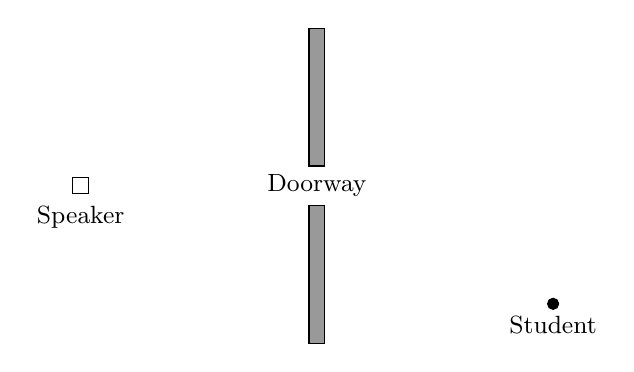
\begin{tikzpicture}[font=\small]
        %% Speaker
        \draw (-3.1,-0.1) rectangle (-2.9,0.1);
        \node[anchor=north,yshift=-1pt] at (-3,-0.1) {Speaker};
        %% Barrier
        \draw[fill=black!40!white] (-0.1,0.25) rectangle (0.1,2);
        \draw[fill=black!40!white] (-0.1,-0.25) rectangle (0.1,-2);
        \node[anchor=center] at (0,0) {Doorway};
        %% Student
        \draw[fill] (3,-1.5) circle (2pt);
        \node[anchor=north,yshift=-1pt] at (3,-1.5) {Student};
    \end{tikzpicture}
    \end{center}
    She notices that she does not have to be directly in front of the doorway to hear the music.
    This spreading of sound waves beyond the doorway is an example of:
    \begin{multicols}{2}
    \begin{choices}
        \wrongchoice{the Doppler effect}
        \wrongchoice{resonance}
        \wrongchoice{refraction}
      \correctchoice{diffraction}
    \end{choices}
    \end{multicols}
\end{question}
}

\element{nysed}{
\begin{question}{June2015-Q32}
    The horn of a moving vehicle produces a sound of constant frequency. 
    Two stationary observers, $A$ and $C$,
        and the vehicle's driver, $B$,
        positioned as represented in the diagram below, hear the sound of the horn.
    \begin{center}
        %% NOTE: insert graphic
        %\includegraphics[width=0.9\columnwidth,keepaspectratio]{June2015-Q32}
    \end{center}
    Compared to the frequency of the sound of the horn heard by driver $B$,
        the frequency heard by observer $A$ is:
    \begin{choices}
        \wrongchoice{lower and the frequency heard by observer $C$ is lower}
        \wrongchoice{lower and the frequency heard by observer $C$ is higher}
        \wrongchoice{higher and the frequency heard by observer $C$ is lower}
        \wrongchoice{higher and the frequency heard by observer $C$ is higher}
    \end{choices}
\end{question}
}


%% Section June2014
%%--------------------
\element{nysed}{
\begin{question}{June2014-Q21}
    What is the period of a sound wave having frequency of \SI{340}{\hertz}?
    \begin{multicols}{2}
    \begin{choices}
      \correctchoice{\SI{2.94e-3}{\second}}
        \wrongchoice{\SI{9.73e-1}{\second}}
        \wrongchoice{\SI{3.40e2}{\second}}
        \wrongchoice{\SI{1.02e2}{\second}}
    \end{choices}
    \end{multicols}
\end{question}
}

\element{nysed}{
\begin{question}{June2014-Q26}
    As a car approaches a pedestrian crossing the road,
        the driver blows the horn.
    Compared to the sound wave emitted by the horn,
        the sound wave detected by the pedestrian has a:
    \begin{choices}
      \correctchoice{higher frequency and a higher pitch}
        \wrongchoice{higher frequency and a lower pitch}
        \wrongchoice{lower frequency and a higher pitch}
        \wrongchoice{lower frequency and a lower pitch}
    \end{choices}
\end{question}
}


%% Section June2013
%%--------------------
\element{nysed}{
\begin{question}{June2013-Q18}
    The energy of a sound wave is most closely related to the wave's:
    \begin{multicols}{2}
    \begin{choices}
        \wrongchoice{frequency}
      \correctchoice{amplitude}
        \wrongchoice{wavelength}
        \wrongchoice{speed}
    \end{choices}
    \end{multicols}
\end{question}
}

\element{nysed}{
\begin{question}{June2013-Q19}
    A sound wave traveling eastward through air causes the air molecules to:
    \begin{choices}
      \correctchoice{vibrate east and west}
        \wrongchoice{vibrate north and south}
        \wrongchoice{move eastward, only}
        \wrongchoice{move northward, only}
    \end{choices}
\end{question}
}

\element{nysed}{
\begin{question}{June2013-Q26}
    Sound waves are produced by the horn of a truck that is approaching a stationary observer.
    Compared to the sound waves detected by the driver of the truck,
        the sound waves detected by the observer have a greater
    \begin{multicols}{2}
    \begin{choices}
        \wrongchoice{wavelength}
        \wrongchoice{period}
      \correctchoice{frequency}
        \wrongchoice{speed}
    \end{choices}
    \end{multicols}
\end{question}
}


%% Section June2012
%%--------------------
\element{nysed}{
\begin{question}{June2012-Q24}
    A tuning fork vibrates at a frequency of \SI{512}{\hertz} when struck with a rubber hammer.
    The sound produced by the tuning fork will travel through the air as a:
    \begin{choices}
      \correctchoice{longitudinal wave with air molecules vibrating parallel to the direction of travel}
        \wrongchoice{transverse wave with air molecules vibrating parallel to the direction of travel}
        \wrongchoice{longitudinal wave with air molecules vibrating perpendicular to the direction of travel}
        \wrongchoice{transverse wave with air molecules vibrating perpendicular to the direction of travel}
    \end{choices}
\end{question}
}

\element{nysed}{
\begin{question}{June2012-Q31}
    What is the wavelength of a \SI{2.50}{\kilo\hertz} sound wave traveling at \SI{326}{\meter\per\second} through air?
    \begin{multicols}{2}
    \begin{choices}
      \correctchoice{\SI{0.130}{\meter}}
        \wrongchoice{\SI{1.30}{\meter}}
        \wrongchoice{\SI{7.67}{\meter}}
        \wrongchoice{\SI{130}{\meter}}
    \end{choices}
    \end{multicols}
\end{question}
}

\element{nysed}{
\begin{question}{June2012-Q33}
    In the diagram below, a stationary source located at point $S$ produces sound having a constant frequency of \SI{512}{\hertz}.
    Observer $A$, \SI{50}{\meter} to the left of $S$,
        hears a frequency of \SI{512}{\hertz}.
    Observer $B$, \SI{100}{\meter} to the right of $S$,
        hears a frequency lower than \SI{512}{\hertz}.
    \begin{center}
    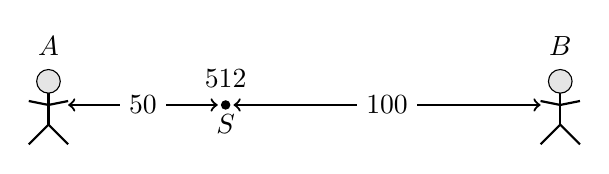
\begin{tikzpicture}
        %% Source
        \draw[fill] (0,0) circle (1.5pt) node[anchor=north] {$S$};
        \node[anchor=south] at (0,0.1) {\SI{512}{\hertz}};
        %% distances
        \draw[thick,<->] (-0.1,0) -- (-2,0) node[pos=0.5,anchor=center,fill=white] {\SI{50}{\meter}};
        \draw[thick,<->] (+0.1,0) -- (4,0) node[pos=0.5,anchor=center,fill=white] {\SI{100}{\meter}};
        %% Labels
        \node[anchor=south] at (-2.25,0.5) {$A$};
        \node[anchor=south] at (+4.25,0.5) {$B$};
        %% Man
        \foreach \x in {-2.25,4.25} {
            \begin{scope}[anchor=south,shift={(\x,-0.5)}]
                \draw[thick] (0,0.25) -- (0,0.75);
                %% Legs
                \draw[thick] (0,0.25) -- (-0.25,0);
                \draw[thick] (0,0.25) -- (+0.25,0);
                %% Arms
                \draw[thick] (0,0.50) -- (-0.25,0.55);
                \draw[thick] (0,0.50) -- (+0.25,0.55);
                %% Head
                \draw[fill=white!90!black] (0,0.80) circle (0.15cm);
            \end{scope}
        }
    \end{tikzpicture}
    \end{center}
    Which statement best describes the motion of the observers?
    \begin{choices}
        \wrongchoice{Observer $A$ is moving toward point $S$, and observer $B$ is stationary.}
        \wrongchoice{Observer $A$ is moving away from point $S$, and observer $B$ is stationary.}
        \wrongchoice{Observer $A$ is stationary, and observer $B$ is moving toward point $S$.}
      \correctchoice{Observer $A$ is stationary, and observer $B$ is moving away from point $S$.}
    \end{choices}
\end{question}
}


%% Section June2011
%%--------------------
\element{nysed}{
\begin{question}{June2011-Q29}
    What is the wavelength of a \SI{256}{\hertz}
        sound wave in air at standard temperature and pressure (STP)?
    \begin{multicols}{2}
    \begin{choices}
        \wrongchoice{\SI{1.17e6}{\meter}}
        \wrongchoice{\SI{0.773}{\meter}}
      \correctchoice{\SI{1.29}{\meter}}
        \wrongchoice{\SI{8.53e-7}{\meter}}
    \end{choices}
    \end{multicols}
\end{question}
}

\element{nysed}{
\begin{question}{June2011-Q31}
    Which statement correctly describes one characteristic of a sound wave?
    \begin{choices}
        \wrongchoice{A sound wave can travel through a vacuum.}
        \wrongchoice{A sound wave is a transverse wave.}
      \correctchoice{The amount of energy a sound wave transmits is directly related to the wave's amplitude.}
        \wrongchoice{The amount of energy a sound wave transmits is inversely related to the wave's frequency.}
    \end{choices}
\end{question}
}


%% Section June2010
%%--------------------


%% Section June2009
%%--------------------
\element{nysed}{
\begin{question}{June2009-Q26}
    The sound wave produced by a trumpet has a frequency of \SI{440}{\hertz}.
    What is the distance between successive compressions in this sound wave as it travels through air at standard temperature and pressure?
    \begin{multicols}{2}
    \begin{choices}
        \wrongchoice{\SI{1.5e-6}{\meter}}
      \correctchoice{\SI{0.75}{\meter}}
        \wrongchoice{\SI{1.3}{\meter}}
        \wrongchoice{\SI{6.8e5}{\meter}}
    \end{choices}
    \end{multicols}
\end{question}
}


%% Section Jan2009
%%--------------------
\element{nysed}{
\begin{question}{Jan2009-Q32}
    A car's horn produces a sound wave of constant frequency.
    As the car speeds up going away from a stationary spectator,
        the sound wave detected by the spectator:
    \begin{choices}
      \correctchoice{decreases in amplitude and decreases in frequency.}
        \wrongchoice{decreases in amplitude and increases in frequency.}
        \wrongchoice{increases in amplitude and decreases in frequency.}
        \wrongchoice{increases in amplitude and increases in frequency.}
    \end{choices}
\end{question}
}


%% Section June2008
%%--------------------
\element{nysed}{
\begin{question}{June2008-Q32}
    A car's horn is producing a sound wave having a constant frequency of \SI{350}{\hertz}.
    If the car moves toward a stationary observer at constant speed,
        the frequency of the car's horn detected by this observer may be:
    \begin{multicols}{2}
    \begin{choices}
        \wrongchoice{\SI{320}{\hertz}}
        \wrongchoice{\SI{350}{\hertz}}
        \wrongchoice{\SI{330}{\hertz}}
      \correctchoice{\SI{380}{\hertz}}
    \end{choices}
    \end{multicols}
\end{question}
}


%% Section Jan2008
%%--------------------
\element{nysed}{
\begin{question}{Jan2008-Q23}
    Increasing the amplitude of a sound wave produced a sound with more:
    \begin{choices}
        \wrongchoice{lower speed}
        \wrongchoice{higher pitch}
        \wrongchoice{shorter wavelength}
      \correctchoice{greater loudness}
    \end{choices}
\end{question}
}

\element{nysed}{
\begin{question}{Jan2008-Q32}
    A police car traveling at a speed of \SI{30.0}{\meter\per\second} sounds its siren,
        which has a frequency of \SI{1.00e3}{\hertz}.
    As the police car approaches a stationary pedestrian,
        the pedestrian detects a siren frequency of:
    \begin{multicols}{2}
    \begin{choices}
        \wrongchoice{\SI{30.0}{\hertz}}
        \wrongchoice{\SI{9.19e2}{\hertz}}
        \wrongchoice{\SI{1.00e3}{\hertz}}
      \correctchoice{\SI{1.10e3}{\hertz}}
    \end{choices}
    \end{multicols}
\end{question}
}

\element{nysed}{
\begin{question}{Jan2008-Q47}
    A sound wave has a wavelength of \SI{5.5}{\meter} as it travels through air at standard temperature and pressure.
    What is the wavelength of this sound in a medium where its speed is \SI{1324}{\meter\per\second}?
    \begin{multicols}{2}
    \begin{choices}
        \wrongchoice{\SI{1.4}{\meter}}
        \wrongchoice{\SI{2.2}{\meter}}
        \wrongchoice{\SI{14}{\meter}}
      \correctchoice{\SI{22}{\meter}}
    \end{choices}
    \end{multicols}
\end{question}
}



%% Section June2007
%%--------------------
\element{nysed}{
\begin{question}{June2007-Q31}
    A student sees a train that is moving away from her and sounding its whistle at a constant frequency.
    Compared to the sound produced by the whistle,
        the sound observed by the student is:
    \begin{choices}
      \correctchoice{lower in pitch}
        \wrongchoice{higher in pitch}
        \wrongchoice{a transverse wave rather than a longitudinal wave}
        \wrongchoice{greater in amplitude}
    \end{choices}
\end{question}
}

\element{nysed}{
\begin{question}{June2007-Q25}
    At an outdoor physics demonstration, a delay of \SI{0.50}{\second} was observed between the time sound waves left a loudspeaker and the time these sound waves reached a student through the air.
    If the air is at standard temperature and pressure,
        how far was the student from the speaker?
    \begin{multicols}{2}
    \begin{choices}
      \correctchoice{\SI{1.7e2}{\meter}}
        \wrongchoice{\SI{1.5e-3}{\meter}}
        \wrongchoice{\SI{6.6e2}{\meter}}
        \wrongchoice{\SI{1.5e8}{\meter}}
    \end{choices}
    \end{multicols}
\end{question}
}



%% Section Jan2007
%%--------------------


%% Section June2006
%%--------------------
\element{nysed}{
\begin{question}{June2006-Q25}
    The energy of a sound wave is most closely related to its:
    \begin{multicols}{2}
    \begin{choices}
      \correctchoice{amplitude}
        \wrongchoice{period}
        \wrongchoice{frequency}
        \wrongchoice{wavelength}
    \end{choices}
    \end{multicols}
\end{question}
}

\element{nysed}{
\begin{question}{June2006-Q26}
    A person observes a fireworks display from a safe distance of \SI{0.750}{\kilo\meter}.
    Assuming that sound travels at \SI{340}{\meter\per\second} in air,
        what is the time between the person seeing and hearing a fireworks explosion?
    \begin{multicols}{2}
    \begin{choices}
      \correctchoice{\SI{2.21}{\second}}
        \wrongchoice{\SI{0.453}{\second}}
        \wrongchoice{\SI{410}{\second}}
        \wrongchoice{\SI{2.55e5}{\second}}
    \end{choices}
    \end{multicols}
\end{question}
}

\element{nysed}{
\begin{question}{June2006-Q48}
    A \SI{512}{\hertz} sound wave travels \SI{100}{\meter} to an observer through air at standard temperature and pressure.
    What is the wavelength of this sound wave?
    \begin{multicols}{2}
    \begin{choices}
      \correctchoice{\SI{0.646}{\meter}}
        \wrongchoice{\SI{0.195}{\meter}}
        \wrongchoice{\SI{1.55}{\meter}}
        \wrongchoice{\SI{5.12}{\meter}}
    \end{choices}
    \end{multicols}
\end{question}
}




%% Section Jan2006
%%--------------------


%% Section June2005
%%--------------------


%% Section Jan2005
%%--------------------
\element{nysed}{
\begin{question}{Jan2005-Q19}
    A train sounds a whistle of constant frequency as it leaves the train station.
    Compared to the sound emitted by the whistle,
        the sound that the passengers standing on the platform hear has a frequency that is:
    \begin{choices}
      \correctchoice{lower, because the sound-wave fronts reach the platform at a frequency lower than the frequency at which they are produced}
        \wrongchoice{lower, because the sound waves travel more slowly in the still air above the platform than in the rushing air near the station.}
        \wrongchoice{higher, because the sound-wave fronts reach the platform at a frequency higher than the frequency at which they are produced.}
        \wrongchoice{higher, because the sound waves travel faster in the still air above the platform than in the rushing air near the station.}
    \end{choices}
\end{question}
}

\element{nysed}{
\begin{question}{Jan2005-Q13}
    A tuning fork vibrating in air produces sound waves.
    These waves are best classified as:
    \begin{choices}
      \correctchoice{longitudinal, because the air molecules are vibrating parallel to the direction of wave motion.}
        \wrongchoice{longitudinal, because the air molecules are vibrating perpendicular to the direction of wave motion.}
        \wrongchoice{transverse, because the air molecules are vibrating parallel to the direction of wave motion.}
        \wrongchoice{transverse, because the air molecules are vibrating perpendicular to the direction of wave motion.}
    \end{choices}
\end{question}
}



%% Section June2004
%%--------------------
\element{nysed}{
\begin{question}{June2004-Q28}
    As a sound wave passes from water,
        where the speed is \SI{1.49e3}{\meter\per\second}, into air, the wave's speed:
    \begin{choices}
      \correctchoice{decreases and its frequency remains the same}
        \wrongchoice{increases and its frequency remains the same}
        \wrongchoice{remains the same and its frequency decreases}
        \wrongchoice{remains the same and its frequency increases}
    \end{choices}
\end{question}
}

\element{nysed}{
\begin{question}{June2004-Q27}
    An electric bell connected to a battery is sealed inside a large jar.
    What happens as the air is removed from the jar?
    \begin{choices}
      \correctchoice{The bell's loudness decreases because sound waves can \emph{not} travel through a vacuum}
        \wrongchoice{The electric circuit stops working because electromagnetic radiation can \emph{not} travel through a vacuum}
        \wrongchoice{The bell's pitch decreases because the frequency of the sound waves is lower in a vacuum than in air}
        \wrongchoice{The bell's loudness increases because of decreased air resistance}
    \end{choices}
\end{question}
}


%% Section Jan2004
%%--------------------
\element{nysed}{
\begin{question}{Jan2004-Q29}
    Which wave phenomena makes it possible for a player to hear the sound from a referee's whistle in an open field even when standing behind the referee?
    \begin{multicols}{2}
    \begin{choices}
      \correctchoice{diffraction}
        \wrongchoice{Doppler effect}
        \wrongchoice{reflection}
        \wrongchoice{refraction}
    \end{choices}
    \end{multicols}
\end{question}
}

\element{nysed}{
\begin{question}{Jan2004-Q41}
    A system consists of an oscillator and a speaker that emits a \SI{1000}{\hertz} sound wave.
    A microphone detects the sound wave \SI{1.00}{\meter} from the speaker.
    \begin{center}
        %% NOTE: complex, keep this
        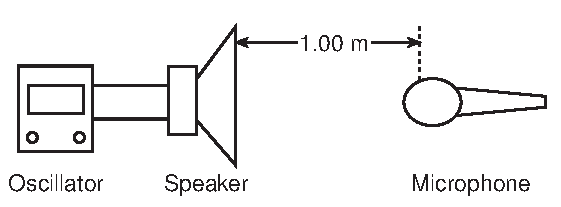
\includegraphics[keepaspectratio,scale=0.75]{Jan2004-Q41}
    \end{center}
    Which type of wave is emitted by the speaker?
    \begin{multicols}{2}
    \begin{choices}
      \correctchoice{longitudinal}
        \wrongchoice{transverse}
        \wrongchoice{circular}
        \wrongchoice{electromagnetic}
    \end{choices}
    \end{multicols}
\end{question}
}

\element{nysed}{
\begin{question}{Jan2004-Q42}
    A system consists of an oscillator and a speaker that emits a \SI{1000}{\hertz} sound wave.
    A microphone detects the sound wave \SI{1.00}{\meter} from the speaker.
    \begin{center}
        %% NOTE: complex, keep this
        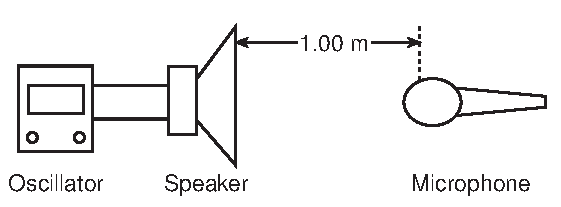
\includegraphics[keepaspectratio,scale=0.75]{Jan2004-Q41}
    \end{center}
    The microphone is moved to a new fixed location \SI{0.50}{\meter} in front of the speaker.
    Compared to the sound waves detected at the \SI{1.00}{\meter} position, the sound waves detected at the \SI{0.50}{\meter} position have a different.
    \begin{multicols}{2}
    \begin{choices}
      \correctchoice{amplitude}
        \wrongchoice{frequency}
        \wrongchoice{wave speed}
        \wrongchoice{wavelength}
    \end{choices}
    \end{multicols}
\end{question}
}

\element{nysed}{
\begin{question}{Jan2004-Q43}
    A system consists of an oscillator and a speaker that emits a \SI{1000}{\hertz} sound wave.
    A microphone detects the sound wave \SI{1.00}{\meter} from the speaker.
    \begin{center}
        %% NOTE: complex, keep this
        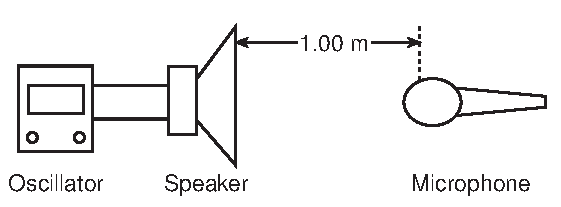
\includegraphics[keepaspectratio,scale=0.75]{Jan2004-Q41}
    \end{center}
    The microphone is moved at constant speed from the \SI{0.50}{\meter} position back to its original position \SI{1.00}{\meter} from the speaker.
    Compared to the \SI{1000}{\hertz} frequency emitted by the speaker,
        the frequency detected by the moving microphone is:
    \begin{multicols}{3}
    \begin{choices}
      \correctchoice{lower}
        \wrongchoice{higher}
        \wrongchoice{the same}
    \end{choices}
    \end{multicols}
\end{question}
}


%% Section June2003
%%--------------------
\element{nysed}{
\begin{question}{June2003-Q30}
    A sound of constant frequency is produce by the siren on top of a firehouse.
    Compared to the frequency produced by the siren,
        the frequency observed by a firefighter approaching the firehouse is:
    \begin{multicols}{3}
    \begin{choices}
      \correctchoice{lower}
        \wrongchoice{higher}
        \wrongchoice{the same}
    \end{choices}
    \end{multicols}
\end{question}
}


%% Section Jan2003
%%--------------------


%% Section Aug2002
%%--------------------
\element{nysed}{
\begin{question}{Aug2002-Q16}
    An electric guitar is generating a sound of constant frequency.
    An increase in which sound wave characteristic would result in an increase in loudness?
    \begin{multicols}{2}
    \begin{choices}
        \wrongchoice{speed}
        \wrongchoice{period}
        \wrongchoice{wavelength}
      \correctchoice{amplitude}
    \end{choices}
    \end{multicols}
\end{question}
}


%% Section June2002
%%--------------------
\element{nysed}{
\begin{question}{June2002-Q29}
    A source of sound waves approaches a stationary observer through a uniform medium.
    Compared to the frequency and wavelength of the emitted sound,
        the observer would detect waves with a:
    \begin{choices}
      \correctchoice{higher frequency and shorter wavelength.}
        \wrongchoice{higher frequency and longer wavelength.}
        \wrongchoice{lower frequency and shorter wavelength.}
        \wrongchoice{lower frequency and longer wavelength.}
    \end{choices}
\end{question}
}


%% Section Jan2002
%%--------------------


%% Section June2001
%%--------------------
\element{nysed}{
\begin{question}{June2001-Q41}
    What type of wave is sound traveling in water?
    \begin{multicols}{2}
    \begin{choices}
        \wrongchoice{torsional}
        \wrongchoice{transverse}
        \wrongchoice{elliptical}
      \correctchoice{longitudinal}
    \end{choices}
    \end{multicols}
\end{question}
}


%% Section Jan2001
%%--------------------
\element{nysed}{
\begin{question}{Jan2001-Q49}
    The driver of a car blows the horn as the car approaches a crosswalk.
    Compared to the actual pitch of the horn,
        the pitch observed by a pedestrian in the crosswalk is:
    \begin{multicols}{3}
    \begin{choices}
        \wrongchoice{lower}
      \correctchoice{higher}
        \wrongchoice{the same}
    \end{choices}
    \end{multicols}
\end{question}
}


%% Section June2000
%%--------------------
\element{nysed}{
\begin{question}{June2000-Q43}
    The diagram below shows a tuning fork vibrating in air.
    The dots represents air molecules as the sound wave moves toward the right.
    \begin{center}
    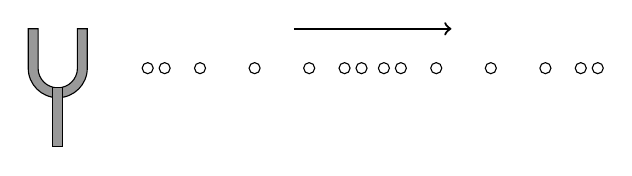
\begin{tikzpicture}
        %% tuning fork
        \begin{scope}[xshift=-1cm,xscale=0.25,yscale=0.25]
            \draw[fill=white!60!black] (-1,2) -- (-1,0) arc (180:360:1) -- (1,2) -- (1.5,2) -- (1.5,0) arc (360:180:1.5) -- (-1.5,2) -- cycle;
            \draw[fill=white!60!black] (-0.25,-1) rectangle (0.25,-4);
        \end{scope}
        %% wave fronts
        \foreach \x in {0,1}
            \foreach \y in {-3,-2,...,3} {
                \draw ({3*\x + (3/(1 + exp(-\y)))},0) circle (2pt);
            }
        %% vector
        \draw[thick,->] (2,0.5) -- (4,0.5);
    \end{tikzpicture}
    \end{center}
    Which diagram best represents the direction of motion of the air molecules?
    \begin{multicols}{2}
    \begin{choices}
        \AMCboxDimensions{down=-0.8cm}
        \wrongchoice{
            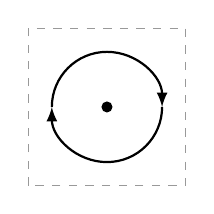
\begin{tikzpicture}[scale=2]
                \draw[dashed,white!60!black] (0,0) rectangle (1,1);
                \fill (0.5,0.5) circle (1pt);
                \draw[thick,-latex] (0.15,0.5) arc (180:0:0.35);
                \draw[thick,-latex] (0.85,0.5) arc (360:180:0.35);
            \end{tikzpicture}
        }
        \wrongchoice{
            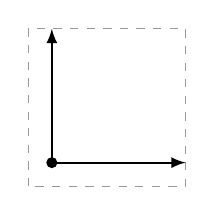
\begin{tikzpicture}[scale=2]
                \draw[dashed,white!60!black] (0,0) rectangle (1,1);
                \fill (0.15,0.15) circle (1pt);
                \draw[thick,-latex] (0.15,0.15) -- (0.15,1);
                \draw[thick,-latex] (0.15,0.15) -- (1,0.15);
            \end{tikzpicture}
        }
        \wrongchoice{
            \begin{tikzpicture}[scale=2]
                \draw[dashed,white!60!black] (0,0) rectangle (1,1);
                \fill (0.5,0.5) circle (1pt);
                \draw[thick,<->] (0.5,1) -- (0.5,0);
            \end{tikzpicture}
        }
        %% ANS is D
        \correctchoice{
            \begin{tikzpicture}[scale=2]
                \draw[dashed,white!60!black] (0,0) rectangle (1,1);
                \fill (0.5,0.5) circle (1pt);
                \draw[thick,<->] (0,0.5) -- (1,0.5);
            \end{tikzpicture}
        }
    \end{choices}
    \end{multicols}
\end{question}
}


%% Section June1999
%%--------------------


%% Section June1998
%%--------------------
\element{nysed}{
\begin{question}{June1998-Q35}
    As a sound wave travels through air,
        there is a net transfer of:
    \begin{choices}
      \correctchoice{energy, only}
        \wrongchoice{mass, only}
        \wrongchoice{both mass and energy}
        \wrongchoice{neither mass nor energy}
    \end{choices}
\end{question}
}


%% Section June1997
%%--------------------
\element{nysed}{
\begin{question}{June1997-Q41}
    The driver of a car sounds the horn while traveling toward a stationary person.
    Compared to the sound heard by the driver,
        the sound heard by the stationary person has:
    \begin{choices}
        \wrongchoice{lower pitch and shorter wavelength}
        \wrongchoice{lower pitch and longer wavelength}
      \correctchoice{higher pitch and shorter wavelength}
        \wrongchoice{higher pitch and longer wavelength}
    \end{choices}
\end{question}
}

\element{nysed}{
\begin{question}{June1997-Q47}
    As shown in the diagram below, speakers $S_1$ and $S_2$,
        separated by a distance of \SI{0.50}{\meter},
        are producing sound of the same frequency.
    A person walking along a path \SI{4.0}{\meter} in front of the speakers hears the sound reach a maximum intensity every \SI{2.0}{\meter}.
    \begin{center}
    \begin{tikzpicture}
        %% NOTE: finish this
    \end{tikzpicture}
    \end{center}
    What is the wavelength of the sound produced by the speakers?
    \begin{multicols}{2}
    \begin{choices}
        \wrongchoice{\SI{1.0}{\meter}}
        \wrongchoice{\SI{0.063}{\meter}}
        \wrongchoice{\SI{0.25}{\meter}}
        \wrongchoice{\SI{4.0}{\meter}}
    \end{choices}
    \end{multicols}
\end{question}
}


%% Section June1996
%%--------------------


%% Section June1995
%%--------------------
\element{nysed}{
\begin{question}{June1995-Q44}
    When an opera singer hits a high pitch note,
        a glass on the opposite side of the opera hall shatters.
    Which statement best explains this phenomenon?
    \begin{choices}
      \correctchoice{The frequency of the note and natural vibration frequency of the glass are equal.}
        \wrongchoice{The vibrations of the note are polarized by the shape of the opera hall.}
        \wrongchoice{The amplitude of the note increases before it reaches the glass.}
        \wrongchoice{The singer and glass are separated by an integral number of wavelengths.}
    \end{choices}
\end{question}
}


%% Section June1994
%%--------------------
\element{nysed}{
\begin{question}{June1994-Q37}
    A characteristic common to sound waves and light waves is that they:
    \begin{multicols}{2}
    \begin{choices}
        \wrongchoice{are longitudinal}
        \wrongchoice{are transverse}
      \correctchoice{transfer energy}
        \wrongchoice{travel in a vacuum}
    \end{choices}
    \end{multicols}
\end{question}
}


%% Section June1986
%%--------------------
\element{nysed}{
\begin{question}{June1986-Q55}
    As the energy imparted to a mechanical wave increases,
        the maximum displacement of the particles in the medium:
    \begin{choices}
        \wrongchoice{decreases}
      \correctchoice{increases}
        \wrongchoice{remains the same}
    \end{choices}
\end{question}
}


%% Section June1985
%%--------------------
\element{nysed}{
\begin{question}{June1985-Q23}
    The driver of a car hears the siren of an ambulance which is moving away from her.
    If the actual frequency of the siren is \SI{2 000}{\hertz},
        the frequency heard by the driver must be:
    \begin{multicols}{2}
    \begin{choices}
      \correctchoice{\SI{1900}{\hertz}}
        \wrongchoice{\SI{2000}{\hertz}}
        \wrongchoice{\SI{1900}{\hertz}}
        \wrongchoice{\SI{4000}{\hertz}}
    \end{choices}
    \end{multicols}
\end{question}
}


\endinput




%% Waves Questions used on the
%% NYSED Physics Regents Examination
%%--------------------------------------------------

%% this section contains 160 problems


%% Section June2015
%%--------------------
\element{nysed}{
\begin{question}{June2015-Q24}
    A student produces a wave in a long spring by vibrating its end.
    As the frequency of the vibration is doubled,
        the wavelength in the spring is:
    \begin{multicols}{2}
    \begin{choices}
        \wrongchoice{quartered}
      \correctchoice{halved}
        \wrongchoice{unchanged}
        \wrongchoice{doubled}
    \end{choices}
    \end{multicols}
\end{question}
}

\element{nysed}{
\begin{question}{June2015-Q25}
    Which two points on the wave shown in the diagram below are in phase with each other?
    \begin{center}
    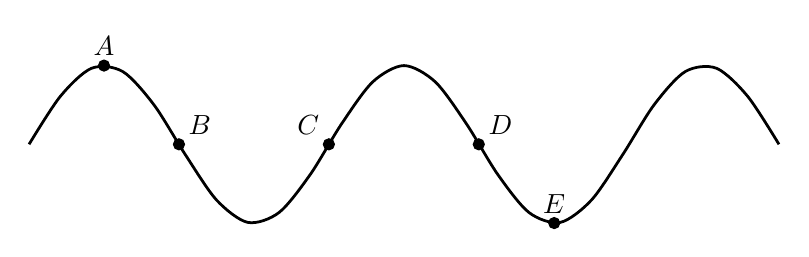
\begin{tikzpicture}[x=0.05\textwidth]
        %% Graph
        \draw[domain=0:5*pi,smooth,line width=1pt] plot (\x, {sin(\x r)});
        %% Labels
        \draw[fill] (1.57,1) circle (2pt) node[anchor=south] {$A$};
        \draw[fill] (3.14,0) circle (2pt) node[anchor=south west] {$B$};
        \draw[fill] (6.28,0) circle (2pt) node[anchor=south east] {$C$};
        \draw[fill] (9.42,0) circle (2pt) node[anchor=south west] {$D$};
        \draw[fill] (11.0,-1) circle (2pt) node[anchor=south] {$E$};
    \end{tikzpicture}
    \end{center}
    \begin{multicols}{2}
    \begin{choices}
        \wrongchoice{$A$ and $B$}
        \wrongchoice{$A$ and $E$}
        \wrongchoice{$B$ and $C$}
      \correctchoice{$B$ and $D$}
    \end{choices}
    \end{multicols}
\end{question}
}

\element{nysed}{
\begin{question}{June2015-Q26}
    As a longitudinal wave moves through a medium,
        the particles of the medium:
    \begin{choices}
      \correctchoice{vibrate parallel to the direction of the wave's propagation.}
        \wrongchoice{vibrate perpendicular to the direction of the wave's propagation.}
        \wrongchoice{are transferred in the direction of the wave’s motion, only.}
        \wrongchoice{are stationary.}
    \end{choices}
\end{question}
}

\element{nysed}{
\begin{question}{June2015-Q27}
    Wind blowing across suspended power lines may cause the power lines to vibrate at their natural frequency.
    This often produces audible sound waves.
    This phenomenon, often called an Aeolian harp,
        is an example of:
    \begin{multicols}{2}
    \begin{choices}
        \wrongchoice{diffraction}
        \wrongchoice{the Doppler effect}
        \wrongchoice{refraction}
      \correctchoice{resonance}
    \end{choices}
    \end{multicols}
\end{question}
}

\element{nysed}{
\begin{question}{June2015-Q35}
    Two pulses approach each other in the same medium.
    The diagram below represents the displacements caused by each pulse.
    \begin{center}
    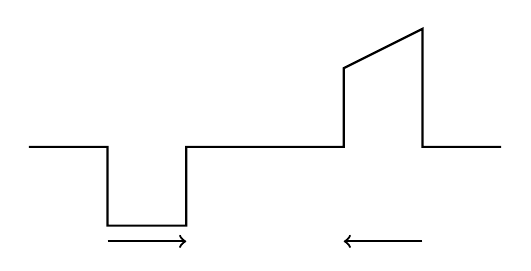
\begin{tikzpicture}
        \draw[thick] (-3,0) -- (-2,0) -- (-2,-1) -- (-1,-1) -- (-1,0) --
                     (+1,0) -- (+1,1) -- (+2,1.5) -- (+2,0) -- (+3,0);
        \draw[thick,->] (-2,-1.2) -- (-1,-1.2);
        \draw[thick,->] (+2,-1.2) -- (+1,-1.2);
    \end{tikzpicture}
    \end{center}
    Which diagram best represents the resultant displacement of the medium as the pulses pass through each other?
    \begin{multicols}{2}
    \begin{choices}
        \AMCboxDimensions{down=-0.5cm}
        \wrongchoice{
            \begin{tikzpicture}
                \draw[white] (-1.5,-0.5) rectangle (1.5,3.0);
                \draw[thick] (-1.5,0) -- (1.5,0);
            \end{tikzpicture}
        }
        \correctchoice{
            \begin{tikzpicture}
                \draw[white] (-1.5,-0.5) rectangle (1.5,3.0);
                \draw[thick] (-1.5,0) -- (-0.5,0) -- (0.5,0.5) -- (0.5,0) --  (1.5,0);
            \end{tikzpicture}
        }
        \wrongchoice{
            \begin{tikzpicture}
                \draw[white] (-1.5,-0.5) rectangle (1.5,3.0);
                \draw[thick] (-1.5,0) -- (-0.5,0) -- (-0.5,2.0) -- (0.5,2.5) -- (0.5,0) --  (1.5,0);
            \end{tikzpicture}
        }
        \wrongchoice{
            \begin{tikzpicture}
                \draw[white] (-1.5,-0.5) rectangle (1.5,3.0);
                \draw[thick] (-1.5,0) -- (-0.5,0) -- (0.5,-0.5) -- (0.5,0) --  (1.5,0);
            \end{tikzpicture}
        }
    \end{choices}
    \end{multicols}
\end{question}
}

\element{nysed}{
\begin{question}{June2015-Q49}
    The diagram below shows waves $A$ and $B$ in the same medium.
    %Wave $A$ and $B$ are represented as a dashed and solid line.
    \begin{center}
    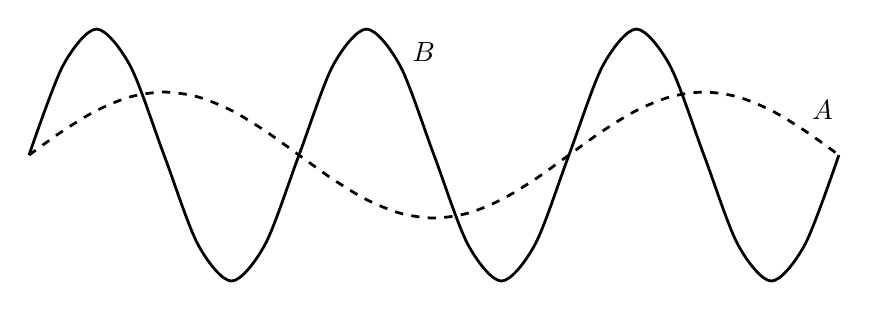
\begin{tikzpicture}[x=0.045\textwidth,yscale=0.8]
        %% Graph
        \draw[domain=0:6*pi,smooth,line width=1pt] plot (\x, {2.0*sin(\x r)});
        \draw[domain=0:6*pi,dashed,smooth,line width=1pt] plot (\x, {sin(0.5*\x r)});
        %% Labels
        \node[anchor=south west] at (8.7,{2.0*sin(8.7 r)})  {$B$};
        \node[anchor=south west] at (18,{sin(0.5*18 r)})  {$A$};
    \end{tikzpicture}
    \end{center}
    Compared to wave $A$, wave $B$ has:
    \begin{choices}
        \wrongchoice{twice the amplitude and twice the wavelength.}
      \correctchoice{twice the amplitude and half the wavelength.}
        \wrongchoice{the same amplitude and half the wavelength.}
        \wrongchoice{half the amplitude and the same wavelength.}
    \end{choices}
\end{question}
}


%% Section June2014
%%--------------------
\element{nysed}{
\begin{question}{June2014-Q17}
    Transverse waves are to radio waves as longitudinal waves are to:
    \begin{multicols}{2}
    \begin{choices}
      \correctchoice{sound waves}
        \wrongchoice{light waves}
        \wrongchoice{microwaves}
        \wrongchoice{ultraviolet waves}
    \end{choices}
    \end{multicols}
\end{question}
}

\element{nysed}{
\begin{question}{June2014-Q25}
    The diagram below represents two identical pulses approaching each other in a uniform medium.
    \begin{center}
    \begin{tikzpicture}
        \begin{axis}[
            clip=false,
            axis y line=left,
            axis x line=center,
            axis line style={->},
            xlabel=\empty,
            xtick=\empty,
            ylabel={displacement},
            y unit=\si{\centi\meter},
            ytick={-6,-3,0,3,6},
            xmin=0,xmax=10,
            ymin=-7,ymax=7,
            grid=major,
            width=0.95\columnwidth,
            height=0.618\columnwidth,
            very thin,
        ]
        \addplot[very thick,domain=0:2]{0};
        \addplot[very thick,domain=4:6]{0};
        \addplot[very thick,domain=8:10]{0};
        %% Waves
        \addplot[very thick,domain=2:4]{-3*(x-2)*(x-4)};
        \addplot[very thick,domain=6:8]{-3*(x-6)*(x-8)};
        %% Arrows
        \draw[very thick,->] (axis cs:2,4) -- (axis cs:4,4);
        \draw[very thick,->] (axis cs:8,4) -- (axis cs:6,4);
        %% Labels
        \node[at={(axis cs:3,4)},above=3pt] {Pulse $A$};
        \node[at={(axis cs:7,4)},above=3pt] {Pulse $B$};
        \end{axis}
    \end{tikzpicture}
    \end{center}
    As the pulses meet and are superposed,
        the maximum displacement of the medium is:
    \begin{multicols}{2}
    \begin{choices}
      \correctchoice{\SI{6}{\centi\meter}}
        \wrongchoice{\SI{0}{\centi\meter}}
        \wrongchoice{\SI{3}{\centi\meter}}
        \wrongchoice{\SI{-6}{\centi\meter}}
    \end{choices}
    \end{multicols}
\end{question}
}

\element{nysed}{
\begin{question}{June2014-Q34}
    The diagram below represents two waves, $A$ and $B$,
        traveling through the same uniform medium.
    \begin{center}
    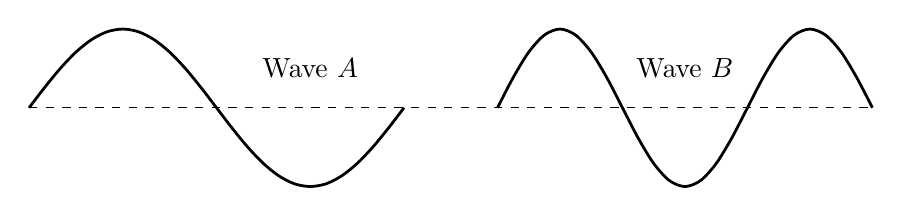
\begin{tikzpicture}[x=0.0625\textwidth]
        %% Graph
        \draw[domain=0:2*pi,smooth,line width=1pt] plot (\x, {sin(\x r)});
        \draw[domain=0:2*pi,smooth,line width=1pt] plot (\x+7.85, {sin(1.5*\x r)});
        \draw[dashed] (0,0) -- (14.13,0);
        %% Labels
        \node[anchor=center] at (4.71,0.5) {Wave $A$};
        \node[anchor=center] at (10.99,0.5) {Wave $B$};
    \end{tikzpicture}
    \end{center}
    Which characteristic is the same for both waves?
    \begin{multicols}{2}
    \begin{choices}
      \correctchoice{amplitude}
        \wrongchoice{period}
        \wrongchoice{wavelength}
        \wrongchoice{frequency}
    \end{choices}
    \end{multicols}
\end{question}
}

\element{nysed}{
\begin{question}{June2014-Q35}
    The diagram below shows a periodic wave.
    \begin{center}
    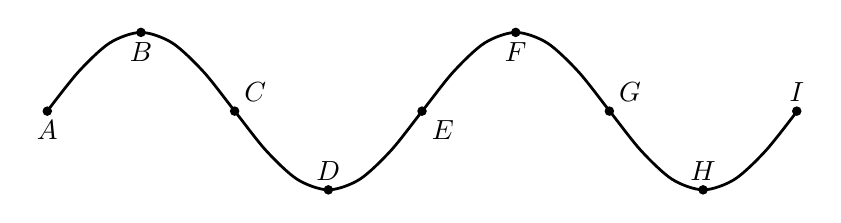
\begin{tikzpicture}[x=0.0625\textwidth]
        %% Graph
        \draw[domain=0:4*pi,smooth,line width=1pt] plot (\x, {sin(\x r)});
        %% Labels
        \node[anchor=north]     at (0,0)    {$A$};
            \draw[fill] (0,0) circle [radius=1.5pt];
        \node[anchor=north]     at (1.57,1) {$B$};
            \draw[fill] (1.57,1) circle [radius=1.5pt];
        \node[anchor=south west]at (3.14,0) {$C$};
            \draw[fill] (3.14,0) circle [radius=1.5pt];
        \node[anchor=south]     at (4.71,-1) {$D$};
            \draw[fill] (4.71,-1) circle [radius=1.5pt];
        \node[anchor=north west]at (6.28,0){$E$};
            \draw[fill] (6.28,0) circle [radius=1.5pt];
        \node[anchor=north]     at (7.85,1){$F$};
            \draw[fill] (7.85,1) circle [radius=1.5pt];
        \node[anchor=south west]at (9.42,0){$G$};
            \draw[fill] (9.42,0) circle [radius=1.5pt];
        \node[anchor=south]     at (10.99,-1){$H$};
            \draw[fill] (10.99,-1) circle [radius=1.5pt];
        \node[anchor=south]     at (12.56,0) {$I$};
            \draw[fill] (12.56,0) circle [radius=1.5pt];
    \end{tikzpicture}
    \end{center}
    Which two points on the wave are \ang{180} out of phase?
    \begin{multicols}{2}
    \begin{choices}
      \correctchoice{$A$ and $C$}
        \wrongchoice{$B$ and $E$}
        \wrongchoice{$F$ and $G$}
        \wrongchoice{$D$ and $H$}
    \end{choices}
    \end{multicols}
\end{question}
}


%% Section June2013
%%--------------------
\element{nysed}{
\begin{question}{June2013-Q20}
    What is the speed of light ($f=\SI{5.09e14}{\hertz}$) in ethyl alcohol?
    \begin{multicols}{2}
    \begin{choices}
        \wrongchoice{\SI{4.53e-9}{\meter\per\second}}
        \wrongchoice{\SI{2.43e2}{\meter\per\second}}
        \wrongchoice{\SI{1.24e8}{\meter\per\second}}
      \correctchoice{\SI{2.21e8}{\meter\per\second}}
    \end{choices}
    \end{multicols}
\end{question}
}

\element{nysed}{
\begin{question}{June2013-Q22}
    The diagram below represents a periodic wave.
    \begin{center}
    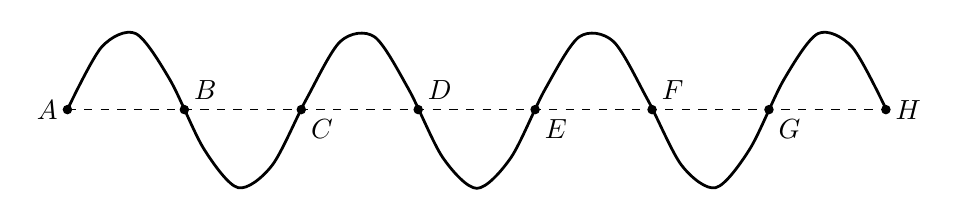
\begin{tikzpicture}[x=0.039\textwidth]
        %% Graph
        \draw[domain=0:7*pi,smooth,line width=1pt] plot (\x, {sin(\x r)});
        \draw[dashed] (0,0) -- (21.98,0);
        %% Circles and Labels
        \draw[fill] (0,0) circle [radius=1.5pt]
            node[anchor=east] {$A$};
        \draw[fill] (3.14,0)  circle [radius=1.5pt]
            node[anchor=south west] {$B$};
        \draw[fill] (6.28,0)  circle [radius=1.5pt]
            node[anchor=north west] {$C$};
        \draw[fill] (9.42,0) circle [radius=1.5pt]
            node[anchor=south west] {$D$};
        \draw[fill] (12.56,0) circle [radius=1.5pt]
            node[anchor=north west] {$E$};
        \draw[fill] (15.7,0) circle [radius=1.5pt]
            node[anchor=south west] {$F$};
        \draw[fill] (18.84,0) circle [radius=1.5pt]
            node[anchor=north west] {$G$};
        \draw[fill] (21.98,0) circle [radius=1.5pt]
            node[anchor=west] {$H$};
    \end{tikzpicture}
    \end{center}
    Which two points on the wave are out of phase?
    \begin{multicols}{2}
    \begin{choices}
        \wrongchoice{$A$ and $C$}
        \wrongchoice{$B$ and $F$}
        \wrongchoice{$C$ and $E$}
      \correctchoice{$D$ and $G$}
    \end{choices}
    \end{multicols}
\end{question}
}

\element{nysed}{
\begin{question}{June2013-Q24}
    A distance of \SI{1.0e-2}{\meter} separates successive crests
        of a periodic wave produced in a shallow tank of water.
    If a crest passes a point in the tank every \SI{4.0e-1}{\second},
        what is the speed of this wave?
    \begin{multicols}{2}
    \begin{choices}
        \wrongchoice{\SI{2.5e-4}{\meter\per\second}}
        \wrongchoice{\SI{4.0e-3}{\meter\per\second}}
      \correctchoice{\SI{2.5e-2}{\meter\per\second}}
        \wrongchoice{\SI{4.0e-1}{\meter\per\second}}
    \end{choices}
    \end{multicols}
\end{question}
}

\element{nysed}{
\begin{question}{June2013-Q48}
    The diagram below shows two waves traveling toward each other
        at equal speed in a uniform medium.
    \begin{center}
    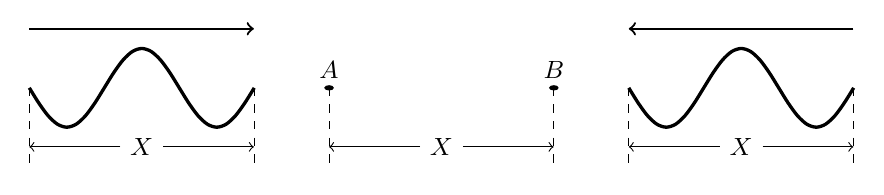
\begin{tikzpicture}[x=0.025\textwidth,yscale=0.5,font=\small]
        %% Wave A
        \draw[domain=0:3*pi,smooth,very thick] plot (\x, {-1*sin(\x r)});
            \draw[thick,->] (0,1.5)   to (9.41,1.5);
        \draw[dashed] (0,0)     to (0,-2);
        \draw[dashed] (9.42,0)  to (9.42,-2);
        \node[anchor=center] (XA) at (4.71,-1.5) {$X$};
            \draw[->] (XA) -- (0,-1.5);
            \draw[->] (XA) -- (9.41,-1.5);
        %% Middle (offset 12.56)
        \node[anchor=south]     at (12.56,0) {$A$};
            \draw[fill] (12.56,0) circle [radius=1.5pt];
        \node[anchor=south]     at (21.98,0) {$B$};
            \draw[fill] (21.98,0) circle [radius=1.5pt];
        \draw[dashed] (12.56,0) -- (12.56,-2);
        \draw[dashed] (21.98,0) -- (21.98,-2);
        \node[anchor=center] (XM) at (17.27,-1.5) {$X$};
            \draw[->] (XM) -- (12.56,-1.5);
            \draw[->] (XM) -- (21.97,-1.5);
        %% Wave B (offset 25.12)
        \draw[domain=0:3*pi,smooth,very thick] plot (\x+25.12, {-1*sin(\x r)});
            \draw[thick,->] (34.53,1.5) -- (25.12,1.5);
        \draw[dashed] (25.12,0)  to (25.12,-2);
        \draw[dashed] (34.54,0)  to (34.54,-2);
        \node[anchor=center] (XB) at (29.83,-1.5) {$X$};
            \draw[->] (XB) -- (25.12,-1.5);
            \draw[->] (XB) -- (34.53,-1.5);
    \end{tikzpicture}
    \end{center}
    When both waves are in the region between points $A$ and $B$,
        they will undergo
    \begin{choices}
        \wrongchoice{diffraction}
        \wrongchoice{the Doppler effect}
        \wrongchoice{destructive interference}
      \correctchoice{constructive interference}
    \end{choices}
\end{question}
}

\element{nysed}{
\begin{question}{June2013-Q49}
    The diagram below shows a series of straight wave fronts produced
        in a shallow tank of water approaching a small opening in
        a barrier.
    \begin{center}
    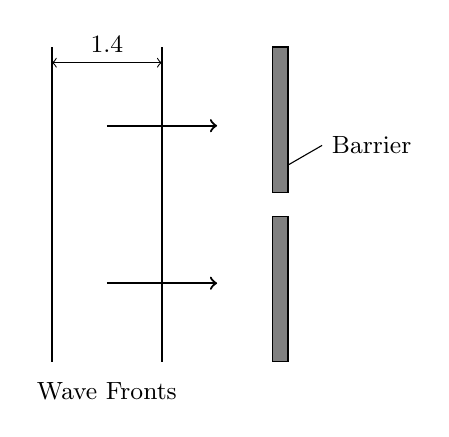
\begin{tikzpicture}[font=\small]
        %% Incoming
        \foreach \x in {0,1.40}
            \draw[thick] (\x,-2) -- (\x,2);
        \draw[thick,->] (0.7,1.0) -- (2.1,1.0);
        \draw[thick,->] (0.7,-1.0) -- (2.1,-1.0);
        %% Barrier
        \draw[fill=black!50!white] (2.8,0.15) rectangle (3.0,2);
        \draw[fill=black!50!white] (2.8,-0.15) rectangle (3.0,-2);
        \draw (3.0,0.5) -- ++ (30:0.5cm)
            node[pos=1.0,anchor=west] {Barrier};
        %% Labels
        \draw[<->] (0,1.8) -- (1.4,1.8)
            node[anchor=south,pos=0.5] {\SI{1.4}{\centi\meter}};
        \node[anchor=north,yshift=-4pt] at (0.7,-2.0) {Wave Fronts};
    \end{tikzpicture}
    \end{center}
    Which diagram represents the appearance of the wave fronts
        after passing through the opening in the barrier?
    \begin{multicols}{2}
    \begin{choices}
        \AMCboxDimensions{down=-2.0cm}
        \wrongchoice{
            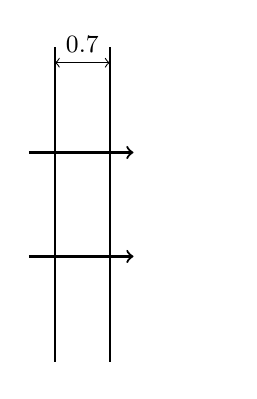
\begin{tikzpicture}[font=\small]
                \draw[white] (-0.33,-2.1) rectangle (2.2,2.1);
                \foreach \x in {0,0.7}
                    \draw[thick] (\x,-2) -- (\x,2);
                \foreach \y in {-0.66,0.66}
                    \draw[thick,->] (-0.33,\y) -- (1.0,\y);
                \draw[<->] (0,1.8) -- (0.7,1.8)
                    node[pos=0.5,anchor=south] {\num{0.7}}
                    node[pos=0.5,anchor=north] {\si{\centi\meter}};
            \end{tikzpicture}
        }
        \wrongchoice{
            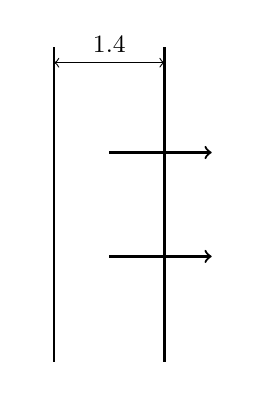
\begin{tikzpicture}[font=\small]
                \draw[white] (-0.33,-2.1) rectangle (2.2,2.1);
                \foreach \x in {0,1.4}
                    \draw[thick] (\x,-2) -- (\x,2);
                \foreach \y in {-0.66,0.66}
                    \draw[thick,->] (0.7,\y) -- (2.0,\y);
                \draw[<->] (0,1.8) -- (1.4,1.8)
                    node[pos=0.5,anchor=south] {\SI{1.4}{\centi\meter}};
            \end{tikzpicture}
        }
        %% Arcs
        \wrongchoice{
            \begin{tikzpicture}[font=\small]
                \draw[white] (-0.33,-2.1) rectangle (2.2,2.1);
                \foreach \x in {0.35,1.05}
                    \draw[thick] (270:\x) arc (-90:90:\x);
                \foreach \d in {45,315}
                    \draw[thick,->] (\d:0.70) -- ++ (\d:0.7);
                \draw[<->] (0:0.35) -- (0:1.05)
                    node[pos=0.5,anchor=south] {\num{0.7}}
                    node[pos=0.5,anchor=north] {\si{\centi\meter}};
            \end{tikzpicture}
        }
        \correctchoice{
            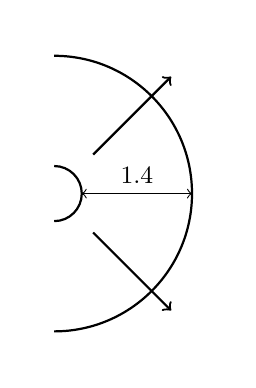
\begin{tikzpicture}[font=\small]
                \draw[white] (-0.33,-2.1) rectangle (2.2,2.1);
                \foreach \x in {0.35,1.75}
                    \draw[thick] (270:\x) arc (-90:90:\x);
                \foreach \d in {45,315}
                    \draw[thick,->] (\d:0.70) -- ++ (\d:1.4);
                \draw[<->] (0:0.35) -- (0:1.75)
                    node[pos=0.5,anchor=south] {\SI{1.4}{\centi\meter}};
            \end{tikzpicture}
        }
    \end{choices}
    \end{multicols}
\end{question}
}


%% Section June2012
%%--------------------
\element{nysed}{
\begin{question}{June2012-Q21}
    The wavelength of a wave doubles as it travels from medium $A$ into medium $B$.
    Compared to the wave in medium $A$,
        the wave in medium $B$ has:
    \begin{choices}
        \wrongchoice{half the speed}
      \correctchoice{twice the speed}
        \wrongchoice{half the frequency}
        \wrongchoice{twice the frequency}
    \end{choices}
\end{question}
}

\element{nysed}{
\begin{question}{June2012-Q29}
    What is characteristic of both sound waves and electromagnetic waves?
    \begin{choices}
        \wrongchoice{They require a medium.}
      \correctchoice{They transfer energy.}
        \wrongchoice{They are mechanical waves.}
        \wrongchoice{They are longitudinal waves.}
    \end{choices}
\end{question}
}

\element{nysed}{
\begin{question}{June2012-Q34}
    While sitting in a boat, a fisherman observes that two complete waves pass by his position every \SI{4}{\second}.
    What is the period of these waves?
    \begin{multicols}{4}
    \begin{choices}
        \wrongchoice{\SI{0.5}{\second}}
      \correctchoice{\SI{2}{\second}}
        \wrongchoice{\SI{8}{\second}}
        \wrongchoice{\SI{4}{\second}}
    \end{choices}
    \end{multicols}
\end{question}
}

\element{nysed}{
\begin{question}{June2012-Q35}
    A wave passes through an opening in a barrier.
    The amount of diffraction experiences by the wave
        depends on the size of the opening and the wave's:
    \begin{multicols}{2}
    \begin{choices}
        \wrongchoice{amplitude}
      \correctchoice{wavelength}
        \wrongchoice{velocity}
        \wrongchoice{phase}
    \end{choices}
    \end{multicols}
\end{question}
}

\element{nysed}{
\begin{question}{June2012-Q46}
    Two speakers, $S_1$ and $S_2$, operating in phase in the same
        medium produce the circular wave patterns shown in the diagram below.
    \begin{center}
    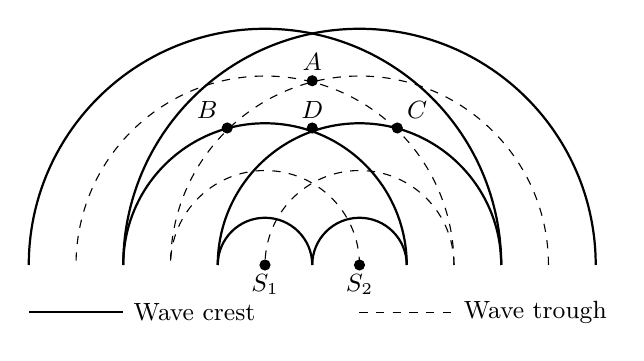
\begin{tikzpicture}[font=\small,scale=1.2]
        \foreach \i in {0.5,1.5,2.5} {
            \draw[thick] (-0.5,0) ++(\i,0) arc(0:180:\i cm);
            \draw[thick] (+0.5,0) ++(\i,0) arc(0:180:\i cm);
        }
        \foreach \j in {1.0,2.0} {
            \draw[dashed] (-0.5,0) ++(\j,0) arc(0:180:\j cm);
            \draw[dashed] (+0.5,0) ++(\j,0) arc(0:180:\j cm);
        }
        %% S_1 and S_2
        \draw[fill] (-0.5,0) circle (1.5pt) node[anchor=north] {$S_1$};
        \draw[fill] (+0.5,0) circle (1.5pt) node[anchor=north] {$S_2$};
        %% A, B, C, D
        \draw[fill] (-0.9,1.45) circle (1.5pt) node[anchor=south east] {$B$};
        \draw[fill] (+0.9,1.45) circle (1.5pt) node[anchor=south west] {$C$};
        \draw[fill] (0,1.95) circle (1.5pt) node[anchor=south] {$A$};
        \draw[fill] (0,1.45) circle (1.5pt) node[anchor=south] {$D$};
        %% Legend
        \draw[thick] (-3,-0.5) -- (-2,-0.5) node[anchor=west] {Wave crest};
        \draw[dashed] (+0.5,-0.5) -- (+1.5,-0.5) node[anchor=west] {Wave trough};
    \end{tikzpicture}
    \end{center}
    At which two points is constructive interference occurring?
    \begin{multicols}{2}
    \begin{choices}
        \wrongchoice{$A$ and $B$}
      \correctchoice{$A$ and $D$}
        \wrongchoice{$B$ and $C$}
        \wrongchoice{$B$ and $D$}
    \end{choices}
    \end{multicols}
\end{question}
}


%% Section June2011
%%--------------------
\element{nysed}{
\begin{question}{June2011-Q16}
    The diagram below represents a view from above of a tank of water in which parallel wave fronts are traveling toward a barrier.
    \begin{center}
    \begin{tikzpicture}
        %% water tank
        \node[anchor=south] at (0,5) {Water Tank};
        \draw[dashed,white!60!black] (-4,0) rectangle (4,5);
        %% wave fronts
        \foreach \x in {-35,-25,-15} \draw (\x mm,0.5) -- (\x mm,4.5);
        \draw[very thick,->] (-4,2) -- (-1,2) node[pos=0.66,anchor=south] {$v$};
        \node[anchor=south] at (-2.5,0) {Wave fronts};
        %% barrier
        \node[anchor=south west,draw,minimum width=1em,minimum height=5.5cm,pattern=vertical lines,rotate=30] (A) at (3.6,0) {};
        \path (A.north east) ++(300:2) node[anchor=south,rotate=-60] {Barrier};
        %% options
        \foreach \x/\y in {180/A,210/B,240/C,270/D} \draw[very thick,->] (3.6,0) ++ (120:{2/sin(60)}) -- ++(\x:2) node[pos=0.75,anchor=center,shift={({\x-90}:1em)}] {$\y$};
    \end{tikzpicture}
    \end{center}
    Which arrow represents the direction of travel for the wave fronts after being reflected from the barrier?
    \begin{multicols}{4}
    \begin{choices}[o]
        \wrongchoice{$A$}
        \wrongchoice{$B$}
      \correctchoice{$C$}
        \wrongchoice{$D$}
    \end{choices}
    \end{multicols}
\end{question}
}

\element{nysed}{
\begin{question}{June2011-Q25}
    A pulse traveled the length of a stretched spring.
    The pulse transferred:
    \begin{choices}
      \correctchoice{energy, only}
        \wrongchoice{mass, only}
        \wrongchoice{both energy and mass}
        \wrongchoice{neither energy nor mass}
    \end{choices}
\end{question}
}

\element{nysed}{
\begin{question}{June2011-Q26}
    The graph below represents the displacement of a particle in
        a medium over a period of time.
    \begin{center}
    \begin{tikzpicture}
        \begin{axis}[
            clip=false,
            axis y line=left,
            axis x line=center,
            axis line style={->},
            xlabel={time},
            x label style={
                at={(current axis.right of origin)},
                anchor=west,
            },
            x unit=\si{\second},
            xtick={1,2,3,4,5,6},
            ylabel={displacement},
            y unit=\si{\centi\meter},
            ytick={-4,-2,0,2,4},
            xmin=0,xmax=6.4,
            ymin=-5,ymax=5,
            width=0.80\columnwidth,
            height=0.45\columnwidth,
            very thin,
        ]
        \addplot[very thick,smooth,domain=0:2*pi]{4*sin(deg(1.56*x))};
        \end{axis}
    \end{tikzpicture}
    \end{center}
    The amplitude of the wave is:
    \begin{multicols}{2}
    \begin{choices}
        \wrongchoice{\SI{4.0}{\second}}
        \wrongchoice{\SI{6.0}{\second}}
        \wrongchoice{\SI{8}{\centi\meter}}
      \correctchoice{\SI{4}{\centi\meter}}
    \end{choices}
    \end{multicols}
\end{question}
}

\element{nysed}{
\begin{question}{June2011-Q27}
    What is the period of a water wave if \num{4.0} complete waves
        pass a fixed point in \SI{10}{\second}?
    \begin{multicols}{2}
    \begin{choices}
        \wrongchoice{\SI{0.25}{\second}}
        \wrongchoice{\SI{0.40}{\second}}
      \correctchoice{\SI{2.5}{\second}}
        \wrongchoice{\SI{4.0}{\second}}
    \end{choices}
    \end{multicols}
\end{question}
}

\element{nysed}{
\begin{question}{June2011-Q28}
    The diagram below represents a periodic wave.
    \begin{center}
    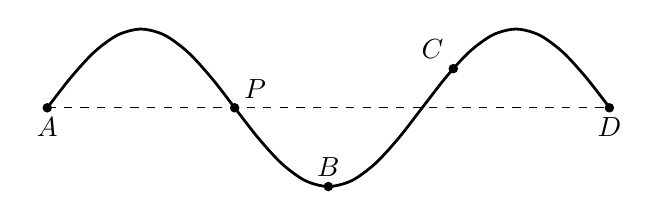
\begin{tikzpicture}[x=0.0625\textwidth]
        %% Graph
        \draw[domain=0:3*pi,smooth,line width=1pt] plot (\x, {sin(\x r)});
        \draw[dashed] (0,0) -- (9.42,0);
        %% Labels
        \node[anchor=north] at (0,0) {$A$};
            \draw[fill] (0,0) circle [radius=1.5pt];
        \node[anchor=south west] at (3.14,0) {$P$};
            \draw[fill] (3.14,0) circle [radius=1.5pt];
        \node[anchor=south] at (4.71,-1) {$B$};
            \draw[fill] (4.71,-1) circle [radius=1.5pt];
        \node[anchor=south east] at (6.804,0.497) {$C$};
            \draw[fill] (6.804,0.497) circle [radius=1.5pt];

        \node[anchor=north] at (9.42,0) {$D$};
            \draw[fill] (9.42,0) circle [radius=1.5pt];
    \end{tikzpicture}
    \end{center}
    Which point on the wave is \ang{90} out of phase with point $P$?
    \begin{multicols}{4}
    \begin{choices}[o]
        \wrongchoice{$A$}
      \correctchoice{$B$}
        \wrongchoice{$C$}
        \wrongchoice{$D$}
    \end{choices}
    \end{multicols}
\end{question}
}

\element{nysed}{
\begin{question}{June2011-Q33}
    Astronauts traveling toward Earth in a fast moving spacecraft
        receive a radio signal from an antenna on Earth.
    Compared to the frequency and wavelength of the radio signal
        from the antenna, the radio signal received by the astronauts has a:
    \begin{choices}
        \wrongchoice{lower frequency and a shorter wavelength}
        \wrongchoice{lower frequency and a longer wavelength}
      \correctchoice{higher frequency and a shorter wavelength}
        \wrongchoice{higher frequency and a longer wavelength}
    \end{choices}
\end{question}
}

\element{nysed}{
\begin{question}{June2011-Q46}
    The diagram below represents a transverse water wave propagating toward the left.
    A cork is floating on the water's surface at point $P$.
    \begin{center}
    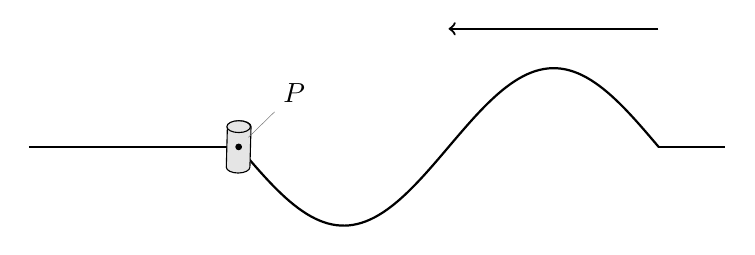
\begin{tikzpicture}[x=0.07\textwidth]
        %% Wave
        \draw[thick] (-3.14,0) -- (0,0);
        \draw[thick,domain=0:2*pi,samples=100] plot (\x, {-1*sin(\x r)});
        \draw[thick] (6.28,0) -- (7.28,0);
        %% Cork
        \node[fill=white!90!black,minimum height=0.5cm,minimum width=0.3cm] (C) at (0,0) {};
        %% make cork 3d
        \draw[fill=white!90!black] (C.south west) arc(180:360:0.15cm and 0.075cm) -- (C.north east) arc(0:180:0.15cm and 0.075cm) -- (C.south west);
        \draw[fill=white!90!black] (C.north) circle (0.15cm and 0.075cm);
        \draw[fill] (0,0) circle (1pt) node[pin=45:$P$] {};
        %% Arrow
        \draw[thick,->] (6.28,1.5) -- (3.14,1.5);
    \end{tikzpicture}
    \end{center}
    In which direction will the cork move as the wave passes point $P$?
    \begin{choices}
        \wrongchoice{up, then down, then up}
      \correctchoice{down, then up, then down}
        \wrongchoice{left, then right, then left}
        \wrongchoice{right, then left, then right}
    \end{choices}
\end{question}
}

\element{nysed}{
\begin{question}{June2011-Q47}
    The diagram below shows a series of wave fronts
        approaching an opening in a barrier.
    Point $P$ is located on the opposite side of the barrier
    \begin{center}
    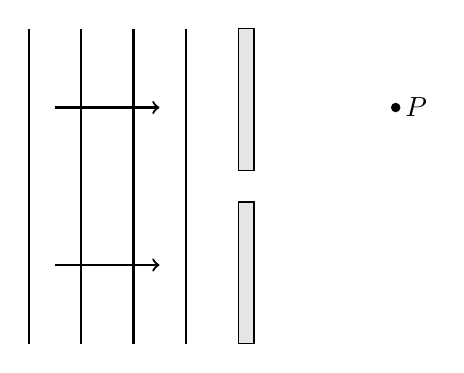
\begin{tikzpicture}
        %% Incoming
        \foreach \i in {0.66,1.33,2.00,2.66} {
            \draw[thick] (-\i,0) -- (-\i,4);
        }
        \draw[thick,->] (-2.33,3) -- (-1.00,3);
        \draw[thick,->] (-2.33,1) -- (-1.00,1);
        %% Barrier
        \draw[fill=white!90!black] (0,0) rectangle (0.2,1.8);
        \draw[fill=white!90!black] (0,2.2) rectangle (0.2,4);
        %% Point P
        \draw[fill] (2,3) circle (1.5pt) node[anchor=west] {$P$};
    \end{tikzpicture}
    \end{center}
    The wave fronts reach point $P$ as a result of:
    \begin{multicols}{2}
    \begin{choices}
        \wrongchoice{resonance}
        \wrongchoice{refraction}
        \wrongchoice{reflection}
      \correctchoice{diffraction}
    \end{choices}
    \end{multicols}
\end{question}
}

\element{nysed}{
\begin{question}{June2011-Q48}
    The diagram below represents a standing wave.
    \begin{center}
    \begin{tikzpicture}[x=0.05\textwidth,yscale=1.0]
        %% Waves
        \draw[domain=0:5*pi,smooth,very thick] plot (\x, {sin(\x r)});
        \draw[domain=0:5*pi,smooth,very thick,dashed] plot (\x, {-1*sin(\x r)});
        %% Walls
        \draw[thick] (0,1) -- (0,-1);
        \draw[thick] (15.7,1) -- (15.7,-1);
        \node[anchor=east,fill,pattern=north east lines,minimum width=0.1cm, minimum height=2cm] at (0,0) {};
        \node[anchor=west,fill,pattern=north east lines,minimum width=0.1cm, minimum height=2cm] at (15.7,0) {};
    \end{tikzpicture}
    \end{center}
    The number of nodes and antinodes shown in the diagram is:
    \begin{choices}
        \wrongchoice{\num{4} nodes and \num{5} antinodes}
        \wrongchoice{\num{5} nodes and \num{6} antinodes}
      \correctchoice{\num{6} nodes and \num{5} antinodes}
        \wrongchoice{\num{6} nodes and \num{10} antinodes}
    \end{choices}
\end{question}
}

\element{nysed}{
\begin{question}{June2011-Q50}
    The diagram below shows two waves traveling in the same medium.
    Points $A$, $B$, $C$, and $D$ are located along the rest position of the medium.
    The waves interfere to produce a resultant wave.
    \begin{center}
    \begin{tikzpicture}
        \begin{axis}[
            clip=false,
            axis y line=left,
            axis x line=center,
            axis line style={->},
            xtick=\empty,
            ylabel={displacement},
            y unit=\si{\meter},
            ytick={-0.3,-0.2,-0.1,0,0.1,0.2,0.3},
            xmin=0,xmax=6.5,
            ymin=-0.35,ymax=0.35,
            width=0.95\columnwidth,
            height=0.618\columnwidth,
            very thin,
        ]
        %% Waves
        \addplot[thick,smooth,domain=0:2*pi]{0.3*sin(deg(x))};
        \addplot[thick,smooth,domain=0:2*pi]{0.1*sin(deg(2*x))};
        %% Labels
        \node[at={(axis cs:0.785,0)},below] {$A$};
        \node[at={(axis cs:2.355,0)},above] {$B$};
        \node[at={(axis cs:3.925,0)},below] {$C$};
        \node[at={(axis cs:5.495,0)},above] {$D$};
        %% Circles
        \draw[fill] (axis cs:0.785,0) circle [radius=1.5pt];
        \draw[fill] (axis cs:2.355,0) circle [radius=1.5pt];
        \draw[fill] (axis cs:3.925,0) circle [radius=1.5pt];
        \draw[fill] (axis cs:5.495,0) circle [radius=1.5pt];
        \end{axis}
    \end{tikzpicture}
    \end{center}
    The superposition of the waves produces the greatest positive
        displacement of the medium from its rest position at point:
    \begin{multicols}{4}
    \begin{choices}[o]
      \correctchoice{$A$}
        \wrongchoice{$B$}
        \wrongchoice{$C$}
        \wrongchoice{$D$}
    \end{choices}
    \end{multicols}
\end{question}
}


%% Section June2010
%%--------------------
\newcommand{\nysedJuneOneZeroQtwentyFour}{
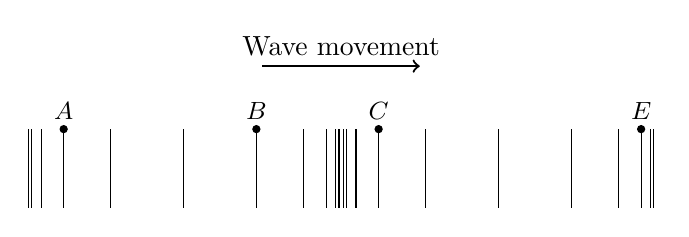
\begin{tikzpicture}
    %% wave fronts
    \foreach \x in {0,1}
        \foreach \y in {-5,-4,...,5} {
            \draw ({4*\x + (4/(1 + exp(-\y)))},0) -- ({4*\x + (4/(1 + exp(-\y)))},1);
        }
    %% wave movement
    \draw[thick,->] (3,1.8) -- (5,1.8) node[pos=0.5,anchor=south] {Wave movement};
    %% options
    \foreach \x/\y/\z in {0/-2/A,0/1/B,1/-2/C,1/3/E}
        \fill ({4*\x + (4/(1 + exp(-\y)))},1) circle (1.5pt) node[anchor=south,font=\small] {$\z$};
\end{tikzpicture}
}

\element{nysed}{
\begin{question}{June2010-Q24}
    A longitudinal wave moves to the right through a uniform medium,
        as shown below.
    Points $A$, $B$, $C$, $D$, and $E$ represent the positions of particles of the medium.
    \begin{center}
        \nysedJuneOneZeroQtwentyFour
    \end{center}
    Which diagram best represents the motion of the particles at position $C$ as the wave moves to the right?
    \begin{multicols}{2}
    \begin{choices}
        \AMCboxDimensions{down=-0.8cm}
        \correctchoice{
            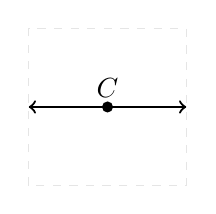
\begin{tikzpicture}[scale=2]
                \draw[dashed,white!90!black] (0,0) rectangle (1,1);
                \fill (0.5,0.5) circle (1pt) node[anchor=south] {$C$};
                \draw[thick,<->] (0,0.5) -- (1,0.5);
            \end{tikzpicture}
        }
        \wrongchoice{
            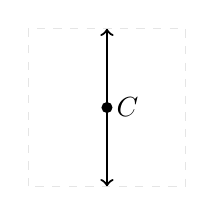
\begin{tikzpicture}[scale=2]
                \draw[dashed,white!90!black] (0,0) rectangle (1,1);
                \fill (0.5,0.5) circle (1pt) node[anchor=west] {$C$};
                \draw[thick,<->] (0.5,0) -- (0.5,1);
            \end{tikzpicture}
        }
        \wrongchoice{
            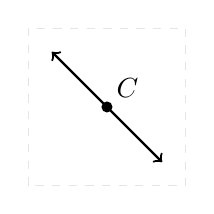
\begin{tikzpicture}[scale=2]
                \draw[dashed,white!90!black] (0,0) rectangle (1,1);
                \fill (0.5,0.5) circle (1pt) node[anchor=south west] {$C$};
                \draw[thick,<->] (0.15,0.85) -- (0.85,0.15);
            \end{tikzpicture}
        }
        \wrongchoice{
            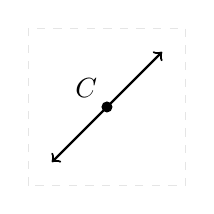
\begin{tikzpicture}[scale=2]
                \draw[dashed,white!90!black] (0,0) rectangle (1,1);
                \fill (0.5,0.5) circle (1pt) node[anchor=south east] {$C$};
                \draw[thick,<->] (0.15,0.15) -- (0.85,0.85);
            \end{tikzpicture}
        }
    \end{choices}
    \end{multicols}
\end{question}
}

\element{nysed}{
\begin{question}{June2010-Q25}
    A longitudinal wave moves to the right through a uniform medium,
        as shown below.
    Points $A$, $B$, $C$, $D$, and $E$ represent the positions of particles of the medium.
    \begin{center}
        \nysedJuneOneZeroQtwentyFour
    \end{center}
    The wavelength of this wave is equal to the distance between points:
    \begin{multicols}{2}
    \begin{choices}
        \wrongchoice{$A$ and $B$}
      \correctchoice{$A$ and $C$}
        \wrongchoice{$B$ and $C$}
        \wrongchoice{$B$ and $E$}
    \end{choices}
    \end{multicols}
\end{question}
}

\element{nysed}{
\begin{question}{June2010-Q26}
    A longitudinal wave moves to the right through a uniform medium,
        as shown below.
    Points $A$, $B$, $C$, $D$, and $E$ represent the positions of particles of the medium.
    \begin{center}
        \nysedJuneOneZeroQtwentyFour
    \end{center}
    The energy of this wave is related to its:
    \begin{multicols}{2}
    \begin{choices}
      \correctchoice{amplitude}
        \wrongchoice{period}
        \wrongchoice{speed}
        \wrongchoice{wavelength}
    \end{choices}
    \end{multicols}
\end{question}
}

\element{nysed}{
\begin{question}{June2010-Q35}
    As viewed from Earth,
        the light from a star has lower frequencies than the lithe emitted by the start because the star is:
    \begin{choices}
        \wrongchoice{moving toward Earth}
      \correctchoice{moving away from Earth}
        \wrongchoice{stationary}
    \end{choices}
\end{question}
}

\element{nysed}{
\begin{question}{June2010-Q48}
    The diagram below represents a periodic wave traveling through a uniform medium.
    \begin{center}
    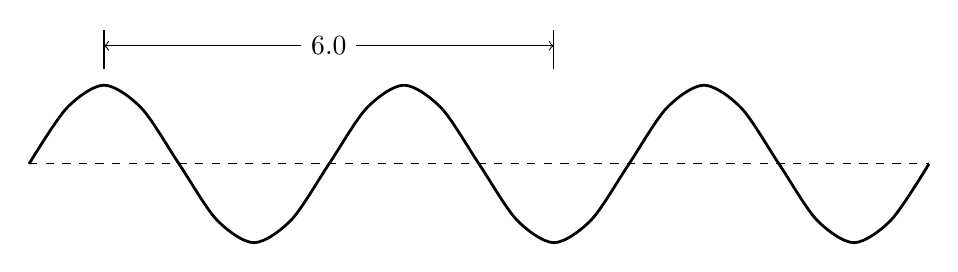
\begin{tikzpicture}[x=0.05\textwidth]
        %% Graph
        \draw[domain=0:6*pi,smooth,line width=1pt] plot (\x, {sin(\x r)});
        \draw[dashed] (0,0) -- (18.84,0);
        %% Labels
        \node[anchor=center] (A) at (6.28,1.5) {\SI{6.0}{\meter}};
        \draw (1.57,1.2) -- (1.57,1.7);
        \draw (10.99,1.2) -- (10.99,1.7);
        \draw[->] (A) -- (1.57,1.5);
        \draw[->] (A) -- (10.99,1.5);
    \end{tikzpicture}
    \end{center}
    If the frequency of the wave is \SI{2.0}{\hertz},
        the speed of the wave is:
    \begin{multicols}{2}
    \begin{choices}
        \wrongchoice{\SI{6.0}{\meter\per\second}}
        \wrongchoice{\SI{2.0}{\meter\per\second}}
      \correctchoice{\SI{8.0}{\meter\per\second}}
        \wrongchoice{\SI{4.0}{\meter\per\second}}
    \end{choices}
    \end{multicols}
\end{question}
}

\element{nysed}{
\begin{question}{June2010-Q50}
    The diagram below shows a standing wave in a string clamped at each end.
    \begin{center}
    \begin{tikzpicture}[x=0.07\textwidth]
        %% Waves
        \draw[domain=0:4*pi,smooth,very thick] plot (\x, {sin(\x r)});
        \draw[domain=0:4*pi,smooth,very thick,dashed] plot (\x, {-1*sin(\x r)});
        %% Walls
        \draw[thick] (0,1) -- (0,-1);
        \draw[thick] (12.56,1) -- (12.56,-1);
        \node[anchor=east,fill,pattern=north east lines,minimum width=0.1cm, minimum height=2cm] at (0,0) {};
        \node[anchor=west,fill,pattern=north east lines,minimum width=0.1cm, minimum height=2cm] at (12.56,0) {};
    \end{tikzpicture}
    \end{center}
    What is the total number of nodes and antinodes in the standing wave?
    \begin{choices}
        \wrongchoice{3 nodes and 2 antinodes}
        \wrongchoice{2 nodes and 3 antinodes}
      \correctchoice{5 nodes and 4 antinodes}
        \wrongchoice{4 nodes and 5 antinodes}
    \end{choices}
\end{question}
}


%% Section June2009
%%--------------------
\element{nysed}{
\begin{question}{June2009-Q24}
    Which type of wave requires a material medium through which to travel?
    \begin{multicols}{2}
    \begin{choices}
      \correctchoice{sound}
        \wrongchoice{radio}
        \wrongchoice{television}
        \wrongchoice{x-ray}
    \end{choices}
    \end{multicols}
\end{question}
}

\element{nysed}{
\begin{question}{June2009-Q25}
    A periodic wave is produced by a vibrating tuning fork.
    The amplitude of the wave would be greater if the tuning fork were:
    \begin{choices}
        \wrongchoice{struck more softly}
      \correctchoice{struck harder}
        \wrongchoice{replaced by a lower frequency tuning fork}
        \wrongchoice{replaced by a higher frequency tuning fork}
    \end{choices}
\end{question}
}

\element{nysed}{
\begin{question}{June2009-Q29}
    The diagram below shows two pulses approaching each other in a uniform medium.
    \begin{center}
    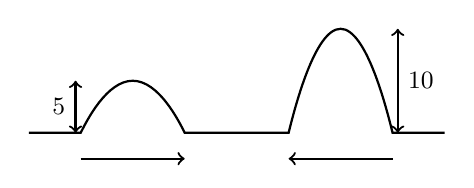
\begin{tikzpicture}[font=\small,scale=0.66]
        \draw[thick] (-4,0) -- (-3,0) parabola bend (-2,1) (-1,0)
                            -- (1,0) parabola bend (2,2) (3,0) -- (4,0);
        %% Arrows
        \draw[thick,->] (-3,-0.5) -- (-1,-0.5);
        \draw[thick,->] (3,-0.5) -- (1,-0.5);
        %% Size Labels
        \draw[thick,<->] (-3.1,0) -- (-3.1,1)
            node[pos=0.5,anchor=east] {\SI{5}{\centi\meter}};
        \draw[thick,<->] (3.1,0) -- (3.1,2)
            node[pos=0.5,anchor=west] {\SI{10}{\centi\meter}};
    \end{tikzpicture}
    \end{center}
    Which diagram best represents the superposition of the two pulses?
    \begin{multicols}{2}
    \begin{choices}
        \AMCboxDimensions{down=-0.5cm}
        \correctchoice{
            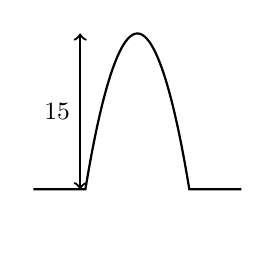
\begin{tikzpicture}[font=\small,scale=0.66]
                \draw[white] (-0.1,-1.1) rectangle (4.1,3.1);
                \draw[thick] (0,0) -- (1,0) parabola bend (2,3) (3,0) -- (4,0);
                \draw[thick,<->] (0.9,0) -- (0.9,3)
                    node[pos=0.5,anchor=east] {\SI{15}{\centi\meter}};
            \end{tikzpicture}
        }
        \wrongchoice{
            \begin{tikzpicture}[font=\small,scale=0.66]
                \draw[white] (-0.1,-1.1) rectangle (4.1,3.1);
                \draw[thick] (0,0) -- (1,0) parabola bend (2,1) (3,0) -- (4,0);
                \draw[thick,<->] (0.9,0) -- (0.9,1)
                    node[pos=0.5,anchor=east] {\SI{5}{\centi\meter}};
            \end{tikzpicture}
        }
        \wrongchoice{
            \begin{tikzpicture}[font=\small,scale=0.66]
                \draw[white] (-0.1,-1.1) rectangle (4.1,3.1);
                \draw[thick] (0,0) -- (1,0) parabola bend (2,1.5) (3,0) -- (4,0);
                \draw[thick,<->] (0.9,0) -- (0.9,1.5)
                    node[pos=0.5,anchor=east] {\SI{7.5}{\centi\meter}};
            \end{tikzpicture}
        }
        \wrongchoice{
            \begin{tikzpicture}[font=\small,scale=0.66]
                \draw[white] (-0.1,-1.1) rectangle (4.1,3.1);
                \draw[thick] (0,0) -- (1,0) parabola bend (2,-1) (3,0) -- (4,0);
                \draw[thick,<->] (0.9,0) -- (0.9,-1)
                    node[pos=0.5,anchor=east] {\SI{5}{\centi\meter}};
            \end{tikzpicture}
        }
    \end{choices}
    \end{multicols}
\end{question}
}


%% Section Jan2009
%%--------------------
\element{nysed}{
\begin{question}{Jan2009-Q23}
    Which type of wave requires a material medium through which to travel?
    \begin{choices}
        \wrongchoice{radio waves}
        \wrongchoice{microwaves}
        \wrongchoice{light waves}
      \correctchoice{mechanical waves}
    \end{choices}
\end{question}
}

\element{nysed}{
\begin{question}{Jan2009-Q25}
    If the amplitude of a wave is increased,
        the frequency of the wave will:
    \begin{choices}
        \wrongchoice{decrease}
        \wrongchoice{increase}
      \correctchoice{stay the same}
    \end{choices}
\end{question}
}

\element{nysed}{
\begin{question}{Jan2009-Q26}
    Which unit is equivalent to a meter per second (\si{\meter\per\second})?
    \begin{choices}
        \wrongchoice{hertz second (\si{\hertz\second})}
      \correctchoice{meter hertz (\si{\meter\hertz})}
        \wrongchoice{second per hertz (\si{\second\per\hertz})}
        \wrongchoice{meter per hertz (\si{\meter\per\hertz})}
    \end{choices}
\end{question}
}

\element{nysed}{
\begin{question}{Jan2009-Q29}
    While playing, two children create a standing wave in a rope,
        as shown in the diagram below.
    A third child participates by jumping rope.
    \begin{center}
        %% NOTE: graphic is necessary
        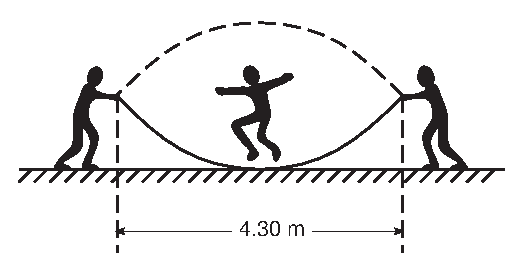
\includegraphics[keepaspectratio,scale=0.75]{Jan2009-Q29}
    \end{center}
    What is the wavelength of this standing wave?
    \begin{multicols}{2}
    \begin{choices}
        \wrongchoice{\SI{2.15}{\meter}}
        \wrongchoice{\SI{4.30}{\meter}}
        \wrongchoice{\SI{6.45}{\meter}}
      \correctchoice{\SI{8.60}{\meter}}
    \end{choices}
    \end{multicols}
\end{question}
}


%% Section June2008
%%--------------------
\element{nysed}{
\begin{question}{June2008-Q25}
    The time required for a wave to complete one full cycle is called the wave's:
    \begin{multicols}{2}
    \begin{choices}
        \wrongchoice{frequency}
        \wrongchoice{velocity}
      \correctchoice{period}
        \wrongchoice{wavelength}
    \end{choices}
    \end{multicols}
\end{question}
}

\element{nysed}{
\begin{question}{June2008-Q27}
    The diagram below represents a transverse wave.
    \begin{center}
    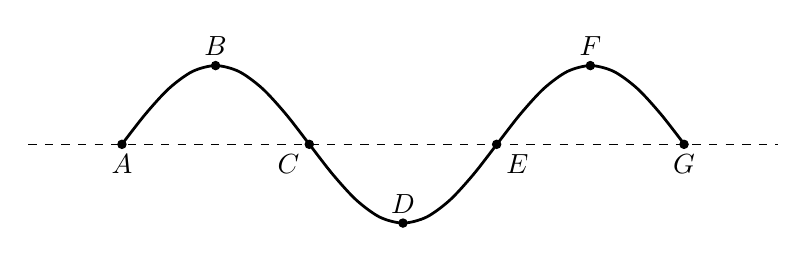
\begin{tikzpicture}[x=0.0625\textwidth]
        %% Graph
        \draw[domain=0:3*pi,smooth,line width=1pt] plot (\x, {sin(\x r)});
        \draw[dashed] (-1.57,0) -- (10.99,0);
        %% Labels
        \node[anchor=north]     at (0,0) {$A$};
        \node[anchor=south]     at (1.57,1) {$B$};
        \node[anchor=north east]at (3.14,0) {$C$};
        \node[anchor=south]     at (4.71,-1) {$D$};
        \node[anchor=north west]at (6.28,0) {$E$};
        \node[anchor=south]     at (7.85,1) {$F$};
        \node[anchor=north]     at (9.42,0) {$G$};
        %% Circles
        \draw[fill] (0,0) circle [radius=1.5pt];
        \draw[fill] (1.57,1) circle [radius=1.5pt];
        \draw[fill] (3.14,0) circle [radius=1.5pt];
        \draw[fill] (4.71,-1) circle [radius=1.5pt];
        \draw[fill] (6.28,0) circle [radius=1.5pt];
        \draw[fill] (7.85,1) circle [radius=1.5pt];
        \draw[fill] (9.42,0) circle [radius=1.5pt];
    \end{tikzpicture}
    \end{center}
    The wavelength of the wave is equal to the distance between points?
    \begin{multicols}{2}
    \begin{choices}
        \wrongchoice{$A$ and $G$}
      \correctchoice{$B$ and $F$}
        \wrongchoice{$C$ and $E$}
        \wrongchoice{$D$ and $F$}
    \end{choices}
    \end{multicols}
\end{question}
}

\element{nysed}{
\begin{question}{June2008-Q30}
    Wave $X$ travels eastward with frequency $f$ and amplitude $A$.
    Wave $Y$, traveling in the same medium,
        interacts with wave $X$ and produces a standing wave.
    Which statement about wave $Y$ is correct?
    \begin{choices}
      \correctchoice{Wave $Y$ must have a frequency of $f$, an amplitude of $A$, and be traveling eastward.}
        \wrongchoice{Wave $Y$ must have a frequency of $2f$, an amplitude of $3A$, and be traveling eastward.}
        \wrongchoice{Wave $Y$ must have a frequency of $3f$, an amplitude of $2A$, and be traveling westward.}
        \wrongchoice{Wave $Y$ must have a frequency of $f$, an amplitude of $A$, and be traveling westward.}
    \end{choices}
\end{question}
}

\element{nysed}{
\begin{question}{June2008-Q31}
    The diagram below represents two pulses approaching each other from opposite directions in the same medium.
    \begin{center}
    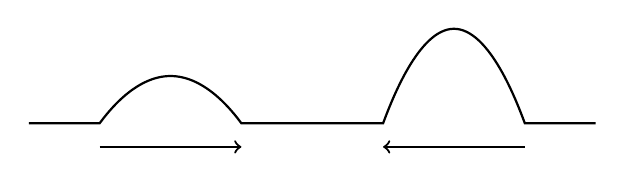
\begin{tikzpicture}[yscale=0.6,xscale=0.9]
        \draw[thick] (-4,0) -- (-3,0) parabola bend (-2,1) (-1,0) -- (1,0) parabola bend (2,2) (3,0) -- (4,0);
        \draw[thick,->] (-3,-0.5) -- (-1,-0.5);
        \draw[thick,->] (3,-0.5) -- (1,-0.5);
    \end{tikzpicture}
    \end{center}
    Which diagram best represents the medium after the pulses have passed through each other?
    \begin{choices}
        \AMCboxDimensions{down=-1.25cm}
        \correctchoice{
            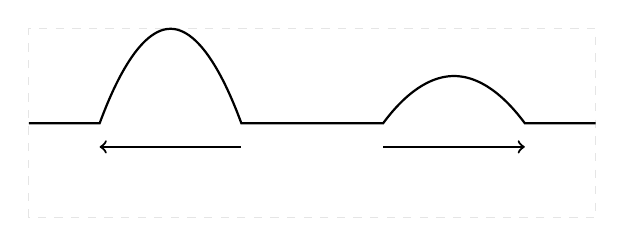
\begin{tikzpicture}[yscale=0.6,xscale=0.9]
                \draw[dashed,white!90!black] (-4,-2) rectangle (4,2);
                \draw[thick] (-4,0) -- (-3,0) parabola bend (-2,2) (-1,0)
                                    -- (1,0) parabola bend (2,1) (3,0) -- (4,0);
                \draw[thick,<-] (-3,-0.5) -- (-1,-0.5);
                \draw[thick,<-] (3,-0.5) -- (1,-0.5);
            \end{tikzpicture}
        }
        \wrongchoice{
            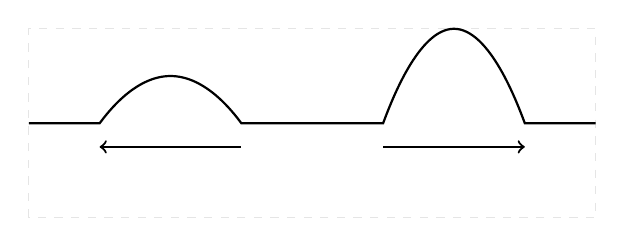
\begin{tikzpicture}[yscale=0.6,xscale=0.9]
                \draw[dashed,white!90!black] (-4,-2) rectangle (4,2);
                \draw[thick] (-4,0) -- (-3,0) parabola bend (-2,1) (-1,0)
                                    -- (1,0) parabola bend (2,2) (3,0) -- (4,0);
                \draw[thick,<-] (-3,-0.5) -- (-1,-0.5);
                \draw[thick,<-] (3,-0.5) -- (1,-0.5);
            \end{tikzpicture}
        }
        \wrongchoice{
            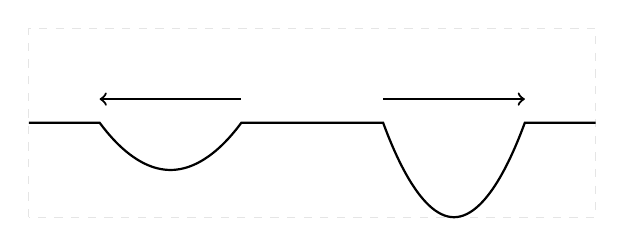
\begin{tikzpicture}[yscale=0.6,xscale=0.9]
                \draw[dashed,white!90!black] (-4,-2) rectangle (4,2);
                \draw[thick] (-4,0) -- (-3,0) parabola bend (-2,-1) (-1,0)
                                    -- (1,0) parabola bend (2,-2) (3,0) -- (4,0);
                \draw[thick,<-] (-3,0.5) -- (-1,0.5);
                \draw[thick,<-] (3,0.5) -- (1,0.5);
            \end{tikzpicture}
        }
        \wrongchoice{
            \begin{tikzpicture}[yscale=0.6,xscale=0.9]
                \draw[dashed,white!90!black] (-4,-2) rectangle (4,2);
                \draw[thick] (-4,0) -- (-3,0) parabola bend (-2,-2) (-1,0)
                                    -- (1,0) parabola bend (2,-1) (3,0) -- (4,0);
                \draw[thick,<-] (-3,0.5) -- (-1,0.5);
                \draw[thick,<-] (3,0.5) -- (1,0.5);
            \end{tikzpicture}
        }
    \end{choices}
\end{question}
}

\element{nysed}{
\begin{question}{June2008-Q48}
    The diagram represents a transverse wave traveling to the right through a medium.
    Point $A$ represents a particle of the medium.
    \begin{center}
    \begin{tikzpicture}[x=0.06\textwidth]
        %% Graph
        \draw[domain=0:3*pi,smooth,very thick] plot (\x, {sin(\x r)});
        \draw[dashed] (0,0) -- (9.42,0);
        %% Vectors
        \draw[thick,->] (3.14,1.0) -- (6.28,1.0)
            node[pos=0.5,anchor=south] {$v$};
        %% Labels
        \draw[fill] (5.50,-0.707) circle [radius=1.5pt]
            node[anchor=north west] {$A$};
    \end{tikzpicture}
    \end{center}
    In which direction will particle $A$ move in the next instance of time?
    \begin{multicols}{2}
    \begin{choices}
        \wrongchoice{up}
      \correctchoice{down}
        \wrongchoice{left}
        \wrongchoice{right}
    \end{choices}
    \end{multicols}
\end{question}
}


%% Section Jan2008
%%--------------------
\element{nysed}{
\begin{question}{Jan2008-Q24}
    The product of a wave's frequency and its period is:
    \begin{multicols}{2}
    \begin{choices}
      \correctchoice{one}
        \wrongchoice{its velocity}
        \wrongchoice{its wavelength}
        \wrongchoice{Planck's constant}
    \end{choices}
    \end{multicols}
\end{question}
}

\element{nysed}{
\begin{question}{Jan2008-Q25}
    A periodic wave having a frequency of \SI{5.0}{\hertz} and a speed of \SI{10}{\meter\per\second} has a wavelength of:
    \begin{multicols}{2}
    \begin{choices}
        \wrongchoice{\SI{0.50}{\meter}}
      \correctchoice{\SI{2.0}{\meter}}
        \wrongchoice{\SI{5.0}{\meter}}
        \wrongchoice{\SI{50}{\meter}}
    \end{choices}
    \end{multicols}
\end{question}
}

\element{nysed}{
\begin{question}{Jan2008-Q31}
    Two pulses traveling in the same uniform medium approach each other,
        as shown in the diagram below.
    \begin{center}
    \begin{tikzpicture}[scale=0.8]
        \draw[thick] (0,0) -- (1,0) -- (2,1) -- (3,0) -- (5,0) -- (6,1) -- (7,0) -- (8,0);
        \draw[thick,->] (1,1.2) -- (3,1.2);
        \draw[thick,->] (7,1.2) -- (5,1.2);
    \end{tikzpicture}
    \end{center}
    Which diagram best represents the superposition of the two pulses?
    \begin{multicols}{2}
    \begin{choices}
        \correctchoice{
            \begin{tikzpicture}[scale=0.8]
                \draw[white] (0,0) rectangle (4,2);
                \draw[thick] (0,0) -- (1,0) -- (2,2) -- (3,0) -- (4,0);
            \end{tikzpicture}
        }
        \wrongchoice{
            \begin{tikzpicture}[scale=0.8]
                \draw[white] (0,0) rectangle (4,2);
                \draw[thick] (0,0) -- (1,0) -- (1,1) -- (3,1) -- (3,0) -- (4,0);
            \end{tikzpicture}
        }
        \wrongchoice{
            \begin{tikzpicture}[scale=0.8]
                \draw[white] (0,0) rectangle (4,2);
                \draw[thick] (0,0) -- (1,0) -- (2,1) -- (3,0) -- (4,0);
            \end{tikzpicture}
        }
        \wrongchoice{
            \begin{tikzpicture}[scale=0.8]
                \draw[white] (0,0) rectangle (4,2);
                \draw[thick] (0,0) -- (4,0);
            \end{tikzpicture}
        }
    \end{choices}
    \end{multicols}
\end{question}
}

\element{nysed}{
\begin{question}{Jan2008-Q34}
    Which diagram best represents the shape and direction of a series of wave fronts after they have passed through a small opening in a barrier?
    \begin{multicols}{2}
    \begin{choices}
        \AMCboxDimensions{down=-0.8cm}
        \wrongchoice{
            \begin{tikzpicture}
                \draw[dashed,white!60!black] (-1.5,-1.2) rectangle (1.5,1.2);
                %% incoming
                \foreach \x in {4,8,12} \draw (-\x mm,-1.2) -- (-\x mm,1.2);
                \foreach \y in {-0.75,0.75} \draw[thick,->] (-1.5,\y) -- (-0.2,\y);
                %% barrier
                \draw[pattern=north east lines] (-0.5ex,-1.2) rectangle (0.5ex,-0.2);
                \draw[pattern=north east lines] (-0.5ex,+1.2) rectangle (0.5ex,+0.2);
                %% outgoing
                \draw[thick,->] (0.5ex,+0.75) -- (1.4,+0.2);
                \draw[thick,->] (0.5ex,-0.75) -- (1.4,-0.2);
                \draw[thick,->] (0.5ex,0) -- (1.2,0);
            \end{tikzpicture}
        }
        \wrongchoice{
            \begin{tikzpicture}
                \draw[dashed,white!60!black] (-1.5,-1.2) rectangle (1.5,1.2);
                %% incoming
                \foreach \x in {4,8,12} \draw (-\x mm,-1.2) -- (-\x mm,1.2);
                \foreach \y in {-0.75,0.75} \draw[thick,->] (-1.5,\y) -- (-0.2,\y);
                %% barrier
                \draw[pattern=north east lines] (-0.5ex,-1.2) rectangle (0.5ex,-0.2);
                \draw[pattern=north east lines] (-0.5ex,+1.2) rectangle (0.5ex,+0.2);
                %% outgoing
                \foreach \x in {4,8,12} \draw (1.5,0) ++(140:\x mm) arc(140:220:\x mm);
                \draw[thick,<-] (1.5,0) ++(150:1ex) -- ++(150:1.3);
                \draw[thick,<-] (1.5,0) ++(210:1ex) -- ++(210:1.3);
            \end{tikzpicture}
        }
        \wrongchoice{
            \begin{tikzpicture}
                \draw[dashed,white!60!black] (-1.5,-1.2) rectangle (1.5,1.2);
                %% incoming
                \foreach \x in {4,8,12} \draw (-\x mm,-1.2) -- (-\x mm,1.2);
                \foreach \y in {-0.75,0.75} \draw[thick,->] (-1.5,\y) -- (-0.2,\y);
                %% barrier
                \draw[pattern=north east lines] (-0.5ex,-1.2) rectangle (0.5ex,-0.2);
                \draw[pattern=north east lines] (-0.5ex,+1.2) rectangle (0.5ex,+0.2);
                %% outgoing
                \foreach \x in {4,8,12} {
                    \draw (0.5ex,0) ++(5:\x mm) arc(5:70:\x mm);
                    \draw (0.5ex,0) ++(355:\x mm) arc(355:290:\x mm);
                }
                \draw[thick,<-] (0.5ex,0) ++ (37:1ex) -- ++(37:1.3);
                \draw[thick,<-] (0.5ex,0) ++ (323:1ex) -- ++(323:1.3);
            \end{tikzpicture}
        }
        %% ANS is D
        \correctchoice{
            \begin{tikzpicture}
                \draw[dashed,white!60!black] (-1.5,-1.2) rectangle (1.5,1.2);
                %% incoming
                \foreach \x in {4,8,12} \draw (-\x mm,-1.2) -- (-\x mm,1.2);
                \foreach \y in {-0.75,0.75} \draw[thick,->] (-1.5,\y) -- (-0.2,\y);
                %% barrier
                \draw[pattern=north east lines] (-0.5ex,-1.2) rectangle (0.5ex,-0.2);
                \draw[pattern=north east lines] (-0.5ex,+1.2) rectangle (0.5ex,+0.2);
                %% outgoing
                \foreach \x in {4,8,12} \draw (0.5ex,0) ++(0,\x mm) arc(90:-90:\x mm);
                \foreach \y in {30,330} \draw[thick,->] (0.5ex,0) ++(\y:0.5ex) -- ++(\y:1.3);
            \end{tikzpicture}
        }
    \end{choices}
    \end{multicols}
\end{question}
}


%% Section June2007
%%--------------------
\element{nysed}{
\begin{question}{June2007-Q22}
    The diagram below represents a transverse wave.
    \begin{center}
    \begin{tikzpicture}[x=0.1\textwidth]
        %% Graph
        \draw[domain=0:2*pi,smooth,very thick] plot (\x, {-1*sin(\x r)});
        \draw[] (0,-1.25) -- (0,1.25);
        \draw[] (0,0) -- (6.28,0);
        %% Labels
        \node[anchor=east]      at (0,0) {$A$};
        \node[anchor=east]      at (0,1) {$D$};
        \node[anchor=east]      at (0,-1) {$E$};
        \node[anchor=north west]at (3.14,0) {$B$};
        \node[anchor=north]     at (6.28,0) {$C$};
        %% Dashed
        \draw[dashed] (0,1) -- (4.71,1);
        \draw[dashed] (0,-1) -- (1.57,-1);
        %% Circles
        \draw[fill] (0,1)   circle [radius=1.5pt];
        \draw[fill] (0,0)   circle [radius=1.5pt];
        \draw[fill] (0,-1)  circle [radius=1.5pt];
        \draw[fill] (3.14,0)circle [radius=1.5pt];
        \draw[fill] (6.28,0)circle [radius=1.5pt];
    \end{tikzpicture}
    \end{center}
    The distance between which two points identifies the amplitude of the wave?
    \begin{multicols}{2}
    \begin{choices}
      \correctchoice{$A$ and $E$}
        \wrongchoice{$A$ and $E$}
        \wrongchoice{$A$ and $C$}
        \wrongchoice{$D$ and $E$}
    \end{choices}
    \end{multicols}
\end{question}
}

\element{nysed}{
\begin{question}{June2007-Q23}
    The diagram below represents a periodic wave.
    \begin{center}
    \begin{tikzpicture}[x=0.0556\textwidth]
        %% Graph
        \draw[domain=0:5*pi,smooth,very thick] plot (\x, {cos(\x r)});
        \draw[] (0,-1.25) -- (0,1.25);
        \draw[] (0,0) -- (16.0,0);
        %% Labels
        \node[anchor=south west]at (0,1) {$A$};
        \node[anchor=north west]at (4.71,0) {$P$};
        \node[anchor=south west]at (7.85,0) {$B$};
        \node[anchor=north west]at (10.99,0) {$C$};
        \node[anchor=south]     at (15.7,-1) {$D$};
        %% Circles
        \draw[fill] (0,1)       circle [radius=1.5pt];
        \draw[fill] (4.71,0)    circle [radius=1.5pt];
        \draw[fill] (7.85,0)    circle [radius=1.5pt];
        \draw[fill] (10.99,0)   circle [radius=1.5pt];
        \draw[fill] (15.7,-1)    circle [radius=1.5pt];
    \end{tikzpicture}
    \end{center}
    Which point on the wave is in phase with point $P$?
    \begin{multicols}{4}
    \begin{choices}[o]
        \wrongchoice{$A$}
        \wrongchoice{$B$}
      \correctchoice{$C$}
        \wrongchoice{$D$}
    \end{choices}
    \end{multicols}
\end{question}
}

\element{nysed}{
\begin{question}{June2007-Q27}
    Which type of wave requires a material medium through which to travel?
    \begin{multicols}{2}
    \begin{choices}
      \correctchoice{sound}
        \wrongchoice{electromagnetic}
        \wrongchoice{infrared}
        \wrongchoice{radio}
    \end{choices}
    \end{multicols}
\end{question}
}

\element{nysed}{
\begin{question}{June2007-Q30}
    Two waves having the same frequency and amplitude are traveling in the same medium.
    Maximum constructive interference occurs at points where the phase difference between the two superposed waves is:
    \begin{multicols}{4}
    \begin{choices}
      \correctchoice{\ang{0}}
        \wrongchoice{\ang{90}}
        \wrongchoice{\ang{180}}
        \wrongchoice{\ang{270}}
    \end{choices}
    \end{multicols}
\end{question}
}


%% Section Jan2007
%%--------------------
\element{nysed}{
\begin{question}{Jan2007-Q21}
    If the amplitude of a wave traveling in a rope is doubled,
        the speed of the wave in the rope will:
    \begin{choices}
      \correctchoice{remain the same}
        \wrongchoice{decrease}
        \wrongchoice{increase}
    \end{choices}
\end{question}
}

\element{nysed}{
\begin{question}{Jan2007-Q22}
    Two waves having the same amplitude and frequency are traveling in the same medium.
    Maximum destructive interference will occur when the phase difference between the waves is:
    \begin{multicols}{4}
    \begin{choices}
      \correctchoice{\ang{180}}
        \wrongchoice{\ang{0}}
        \wrongchoice{\ang{270}}
        \wrongchoice{\ang{90}}
    \end{choices}
    \end{multicols}
\end{question}
}

\element{nysed}{
\begin{question}{Jan2007-Q24}
    A ringing bell is located in a chamber.
    When the air is removed from the chamber,
        why can the bell be seen vibrating but \emph{not} be heart?
    \begin{choices}
      \correctchoice{Light waves can travel through a vacuum, but sound waves cannot.}
        \wrongchoice{Light waves travel slower than sound waves.}
        \wrongchoice{Sound waves have greater amplitude than light waves.}
        \wrongchoice{Sound waves have higher frequency than light waves.}
    \end{choices}
\end{question}
}

\element{nysed}{
\begin{question}{Jan2007-Q25}
    As a transverse wave travels through a medium,
        the individual particles of the medium move:
    \begin{choices}
      \correctchoice{perpendicular to the direction of wave travel}
        \wrongchoice{parallel to the direction of wave travel}
        \wrongchoice{in circles}
        \wrongchoice{in ellipses}
    \end{choices}
\end{question}
}

\element{nysed}{
\begin{question}{Jan2007-Q28}
    Parallel wave fronts incident on an opening in a barrier are diffracted.
    For which combination of wavelength and size of opening will diffraction effects be greatest?
    \begin{choices}
      \correctchoice{long wavelength and narrow opening}
        \wrongchoice{long wavelength and wide opening}
        \wrongchoice{short wavelength and narrow opening}
        \wrongchoice{short wavelength and wide opening}
    \end{choices}
\end{question}
}

\element{nysed}{
\begin{question}{Jan2007-Q49}
    The diagram below represents a wave.
    \begin{center}
    \begin{tikzpicture}[x=0.035\textwidth]
        %% Wave
        \draw[domain=0:6*pi,smooth,very thick] plot (\x, {sin(\x r)});
        %% Y Label
        \draw (0,-1.5) -- (0,1.2);
        \draw (18.84,-1.5) -- (18.84,1.2);
        \node[anchor=east] (X1) at (-0.5,1.0) {\SI{0.20}{\meter}};
        \node[anchor=east] (X2) at (-0.5,-1.0) {\SI{-0.20}{\meter}};
        \draw[dashed] (X1) -- (18.84,1.0);
        \draw[dashed] (X2) -- (18.84,-1.0);
        \draw[dashed] (0,0) -- (18.84,0.0);
        %% X Label
        \node[anchor=center] (X4) at (9.42,-1.3) {\SI{6.00}{\meter}};
        \draw[->] (X4) -- (0,-1.3);
        \draw[->] (X4) -- (18.84,-1.3);
    \end{tikzpicture}
    \end{center}
    What is the speed of the wave if its frequency is \SI{8.0}{\hertz}?
    \begin{multicols}{2}
    \begin{choices}
      \correctchoice{\SI{16}{\meter\per\second}}
        \wrongchoice{\SI{48}{\meter\per\second}}
        \wrongchoice{\SI{1.6}{\meter\per\second}}
        \wrongchoice{\SI{3.2}{\meter\per\second}}
    \end{choices}
    \end{multicols}
\end{question}
}


%% Section June2006
%%--------------------
\element{nysed}{
\begin{question}{June2006-Q28}
    The diagram below represents straight fronts passing from deep water into shallow water,
        with a change in speed and direction.
    \begin{center}
    \begin{tikzpicture}
        %% deep water
        \draw[thick,latex-]  (1,2) -- (1,3.5) node[anchor=north] {Deep water};
        \foreach \y in {1.5,2.0,2.5,3.0} \draw[thick] (0,\y) -- ({1.5*(\y+0.66)},\y) -- ++(20:{2.3-1.85*(\y-3)});
        %% boundary
        \draw[line width=2pt] (1,0) -- (7,4) node[pos=0.2,anchor=north,rotate=34] {Boundary};
        \draw[thick,-latex] (1,0) ++(33.69:5.5) ++(290:1ex) -- ++(290:1) node[anchor=north] {Shallow water};
    \end{tikzpicture}
    \end{center}
    Which phenomenon is illustrated in the diagram?
    \begin{multicols}{2}
    \begin{choices}
      \correctchoice{refraction}
        \wrongchoice{reflection}
        \wrongchoice{diffraction}
        \wrongchoice{interference}
    \end{choices}
    \end{multicols}
\end{question}
}

\element{nysed}{
\begin{question}{June2006-Q32}
    Two waves traveling in the same medium and having the same wavelength ($\lambda$) interfere to create a standing wave.
    What is the distance between two consecutive nodes on this standing wave?
    \begin{multicols}{4}
    \begin{choices}
      \correctchoice{$\dfrac{\lambda}{2}$}
        \wrongchoice{$\lambda$}
        \wrongchoice{$\dfrac{\lambda}{4}$}
        \wrongchoice{$\dfrac{3\lambda}{4}$}
    \end{choices}
    \end{multicols}
\end{question}
}

\element{nysed}{
\begin{question}{June2006-Q33}
    An earthquake wave is traveling from west to east through rock.
    If the particles of the rock are vibrating in a north-south direction,
        the wave must be classified as:
    \begin{multicols}{2}
    \begin{choices}
      \correctchoice{transverse}
        \wrongchoice{longitudinal}
        \wrongchoice{a microwave}
        \wrongchoice{a radio wave}
    \end{choices}
    \end{multicols}
\end{question}
}

\element{nysed}{
\begin{question}{June2006-Q46}
    The diagram represents two pulses approaching each other.
    \begin{center}
    \begin{tikzpicture}[scale=0.8]
        \draw[thick] (0,0) -- (1,0) -- (1,1) -- (2,1) -- (2,0) -- (4,0) -- (4,-2) -- (5,-2) -- (5,0) -- (6,0);
        \draw[thick,->] (1,1.5) -- (2,1.5);
        \draw[thick,->] (5,1.5) -- (4,1.5);
    \end{tikzpicture}
    \end{center}
    Which diagram best represents the resultant pulse at the instant the pulses are passing through each other?
    \begin{multicols}{2}
    \begin{choices}
        \AMCboxDimensions{down=-1.5cm}
        \correctchoice{
            \begin{tikzpicture}[scale=0.8]
                \draw[white] (0,-2) rectangle (3,1);
                \draw[thick] (0,0) -- (1,0) -- (1,-1) -- (2,-1) -- (2,0) -- (3,0);
            \end{tikzpicture}
        }
        \wrongchoice{
            \begin{tikzpicture}[scale=0.8]
                \draw[white] (0,-2) rectangle (3,1);
                \draw[thick] (0,0) -- (1,0) -- (1,-2) -- (2,-2) -- (2,0) -- (3,0);
            \end{tikzpicture}
        }
        \wrongchoice{
            \begin{tikzpicture}[scale=0.8]
                \draw[white] (0,-2) rectangle (3,1);
                \draw[thick] (0,0) -- (1,0) -- (1,1) -- (2,1) -- (2,0) -- (3,0);
            \end{tikzpicture}
        }
        \wrongchoice{
            \begin{tikzpicture}[scale=0.8]
                \draw[white] (0,-2) rectangle (3,1);
                \draw[thick] (0,0) -- (3,0);
            \end{tikzpicture}
        }
    \end{choices}
    \end{multicols}
\end{question}
}


%% Section Jan2006
%%--------------------
\element{nysed}{
\begin{question}{Jan2006-Q28}
    A sonar wave is reflected from the ocean floor.
    For which angles of incidence do the wave's angle of reflection equal its angle of incidence?
    \begin{choices}
        \wrongchoice{angles less than \ang{45}, only}
        \wrongchoice{an angle of \ang{45}, only}
        \wrongchoice{angles greater than \ang{45}, only}
      \correctchoice{all angles of incidence}
    \end{choices}
\end{question}
}

\element{nysed}{
\begin{question}{Jan2006-Q29}
    How are electromagnetic waves that are produced by oscillating charges and sound waves that are produced by oscillating tuning forks similar?
    \begin{choices}
      \correctchoice{Both have the same frequency as their respective sources.}
        \wrongchoice{Both require a matter medium for propagation.}
        \wrongchoice{Both are longitudinal waves.}
        \wrongchoice{Both are transverse waves.}
    \end{choices}
\end{question}
}

\element{nysed}{
\begin{question}{Jan2006-Q30}
    The diagram below represents a transverse wave traveling in a string.
    \begin{center}
    \begin{tikzpicture}[x=0.0625\textwidth]
        %% Graph
        \draw[domain=0:4*pi,smooth,line width=1pt] plot (\x, {sin(\x r)});
        \draw (0,0) -- (13.00,0);
        \draw (0,-1.2) -- (0,1.2);
        %% Labels
        \node[anchor=north west]at (0,0)    {$A$};
            \draw[fill] (0,0) circle [radius=1.5pt];
        \node[anchor=north]     at (1.57,1) {$B$};
            \draw[fill] (1.57,1) circle [radius=1.5pt];
        \node[anchor=south west]at (3.14,0) {$C$};
            \draw[fill] (3.14,0) circle [radius=1.5pt];
        \node[anchor=south]     at (4.71,-1) {$D$};
            \draw[fill] (4.71,-1) circle [radius=1.5pt];
        \node[anchor=north west]at (6.28,0){$E$};
            \draw[fill] (6.28,0) circle [radius=1.5pt];
        \node[anchor=north]     at (7.85,1){$F$};
            \draw[fill] (7.85,1) circle [radius=1.5pt];
        \node[anchor=south west]at (9.42,0){$G$};
            \draw[fill] (9.42,0) circle [radius=1.5pt];
        \node[anchor=south]     at (10.99,-1){$H$};
            \draw[fill] (10.99,-1) circle [radius=1.5pt];
    \end{tikzpicture}
    \end{center}
    Which two labeled points are \ang{180} out of phase?
    \begin{multicols}{2}
    \begin{choices}
      \correctchoice{$D$ and $F$}
        \wrongchoice{$B$ and $F$}
        \wrongchoice{$A$ and $D$}
        \wrongchoice{$D$ and $H$}
    \end{choices}
    \end{multicols}
\end{question}
}

\element{nysed}{
\begin{question}{Jan2006-Q32}
    The diagram below represents shallow water waves of constant wavelength passing through two small opening, $A$ and $B$, in a barrier.
    \begin{center}
    %% NOTE: June1996-Q42
    \begin{tikzpicture}
        %% incoming
        \foreach \x in {5,15}
            \draw[dashed] (-4,-\x mm) -- (4,-\x mm);
        \foreach \x in {10,20}
            \draw[thick] (-4,-\x mm) -- (4,-\x mm);
        %% outcoming A
        \foreach \x in {5,15,25}  {
            \draw[dashed] (-1,0.25ex) ++(\x mm,0) arc (0:180:\x mm);
            \draw[dashed] (+1,0.25ex) ++(\x mm,0) arc (0:180:\x mm);
        }
        \foreach \x in {10,20,30} {
            \draw[thick] (-1,0.25ex) ++(\x mm,0) arc (0:180:\x mm);
            \draw[thick] (+1,0.25ex) ++(\x mm,0) arc (0:180:\x mm);
        }
        %% barrier
        \draw[fill=white!50!black] (-4,-0.25ex) rectangle (-1.1,0.25ex);
        \draw[fill=white!50!black] (-0.9,-0.25ex) rectangle (0.9,0.25ex);
        \draw[fill=white!50!black] (1.1,-0.25ex) rectangle (4.0,0.25ex);
        %% labels
        \node[anchor=north] at (-1,0) {$A$};
        \node[anchor=north] at (+1,0) {$B$};
        \fill (6.8mm,25.3mm) circle (2pt) node[anchor=south west] {$P$};
        %% Legend
        \draw (-2.5,-2.5) -- (-1.5,-2.5) node[anchor=west] {Crests};
        \draw[dashed] (0.5,-2.5) -- (1.5,-2.5) node[anchor=west] {Troughs};
    \end{tikzpicture}
    \end{center}
    Which statement best describes the interference at point $P$?
    \begin{choices}
      \correctchoice{It is destructive, and causes a decrease in amplitude.}
        \wrongchoice{It is destructive, and causes a shorter wavelength.}
        \wrongchoice{It is constructive, and causes an increase in amplitude.}
        \wrongchoice{It is constructive, and causes a longer wavelength.}
    \end{choices}
\end{question}
}


%% Section June2005
%%--------------------
\element{nysed}{
\begin{question}{June2005-Q24}
    A transverse wave passes through a uniform material medium from left to right,
        as shown in the diagram below.
    \begin{center}
    \begin{tikzpicture}[x=0.0625\textwidth]
        %% Wave
        \draw[domain=0:3.5*pi,smooth,line width=1pt] plot (\x, {sin(\x r)});
        %% Vector
        \draw[->] (4.0,1.5) -- (7.0,1.5)
            node[pos=0.5,anchor=south] {$v$};
    \end{tikzpicture}
    \end{center}
    Which diagram best represents the direction of vibration of the particles of the medium?
    \begin{multicols}{2}
    \begin{choices}
        \AMCboxDimensions{down=-0.8cm}
        \correctchoice{
            \begin{tikzpicture}
                \draw[dashed,white!90!black] (-1,-1) rectangle (1,1);
                \draw[fill] (0,0) circle (1pt);
                \draw[thick,<->] (270:1) -- (90:1);
            \end{tikzpicture}
        }
        \wrongchoice{
            \begin{tikzpicture}
                \draw[dashed,white!90!black] (-1,-1) rectangle (1,1);
                \draw[fill] (0,0) circle (1pt);
                \draw[thick,<->] (135:1) -- (315:1);
            \end{tikzpicture}
        }
        \wrongchoice{
            \begin{tikzpicture}
                \draw[dashed,white!90!black] (-1,-1) rectangle (1,1);
                \draw[fill] (0,0) circle (1pt);
                \draw[thick,<->] (180:1) -- (0:1);
            \end{tikzpicture}
        }
        \wrongchoice{
            \begin{tikzpicture}
                \draw[dashed,white!90!black] (-1,-1) rectangle (1,1);
                \draw[fill] (0,0) circle (1pt);
                \draw[thick,<->] (225:1) -- (45:1);
            \end{tikzpicture}
        }
    \end{choices}
    \end{multicols}
\end{question}
}

\element{nysed}{
\begin{question}{June2005-Q29}
    If the speed of a wave doubles as it passes from shallow water into deeper water,
        its wavelength will be:
    \begin{multicols}{2}
    \begin{choices}
      \correctchoice{doubled}
        \wrongchoice{unchanged}
        \wrongchoice{halved}
        \wrongchoice{quadrupled}
    \end{choices}
    \end{multicols}
\end{question}
}


%% Section Jan2005
%%--------------------
\element{nysed}{
\begin{question}{Jan2005-Q10}
    The diagram below shows two pulses of equal amplitude, $A$,
        approaching point $P$ along a uniform string.
    \begin{center}
    \begin{tikzpicture}[font=\small,scale=0.90]
        \draw[thick] (-4,0) -- (-3,0) parabola bend (-2,1) (-1,0)
                            -- (1,0) parabola bend (2,-1) (3,0) -- (4,0);
        \draw[dashed] (-4,0) -- (4,0);
        %% Arrows
        \draw[thick,->] (-2,1.3) -- ++(0:1cm);
        \draw[thick,->] (2,-1.3) -- ++(180:1cm);
        %% String label
        \node[anchor=north west] at (-4,0) {String};
        \draw[fill] (0,0) circle (1pt)
            node[anchor=south] {$P$};
        %% Size Labels
        \draw[thick,<->] (-2.0,0) -- (-2.0,1)
            node[pos=0.5,anchor=east] {$A$};
        \draw[thick,<->] (2.0,0) -- (2.0,-1)
            node[pos=0.5,anchor=west] {$A$};
    \end{tikzpicture}
    \end{center}
    When the two pulses meet at $P$,
        the vertical displacement of the string at $P$ will be:
    \begin{multicols}{4}
    \begin{choices}
      \correctchoice{$0$}
        \wrongchoice{$2A$}
        \wrongchoice{$\dfrac{A}{2}$}
        \wrongchoice{$A$}
    \end{choices}
    \end{multicols}
\end{question}
}

\element{nysed}{
\begin{question}{Jan2005-Q11}
    The energy of a water wave is most closely related to its:
    \begin{multicols}{2}
    \begin{choices}
      \correctchoice{amplitude}
        \wrongchoice{frequency}
        \wrongchoice{wavelength}
        \wrongchoice{period}
    \end{choices}
    \end{multicols}
\end{question}
}

\element{nysed}{
\begin{question}{Jan2005-Q12}
    Which form(s) of energy can be transmitted through a vacuum?
    \begin{choices}
      \correctchoice{light, only}
        \wrongchoice{sound, only}
        \wrongchoice{both light and sound}
        \wrongchoice{neither light nor sound}
    \end{choices}
\end{question}
}

\element{nysed}{
\begin{question}{Jan2005-Q18}
    The diagram below represents a wave moving toward the right side of the page.
    \begin{center}
    %% NOTE: Cannot use relative x and y
    \begin{tikzpicture}[xscale=0.25,yscale=0.75]
        \draw[domain=0:3*pi,smooth,line width=1pt] plot (\x, {sin(\x r)});
        \draw[thick,->] (3.14,1.5) -- (6.28,1.5);
    \end{tikzpicture}
    \end{center}
    Which wave shown below could produce a standing wave with the original wave?
    \begin{multicols}{2}
    \begin{choices}
        \AMCboxDimensions{down=-1.0cm}
        \correctchoice{
            \begin{tikzpicture}[xscale=0.25,yscale=0.75]
                \draw[white] (-1.5,-1.5) rectangle (9.42,1.50);
                \draw[domain=0:3*pi,smooth,line width=1pt] plot (\x, {sin(\x r)});
                \draw[->] (6.28,1.5) -- (3.14,1.5);
            \end{tikzpicture}
        }
        \wrongchoice{
            \begin{tikzpicture}[xscale=0.25,yscale=0.75]
                \draw[white] (-1.5,-1.5) rectangle (9.42,1.50);
                \draw[domain=0:3*pi,smooth,line width=1pt] plot (\x, {sin(\x r)});
                \draw[thick,->] (3.14,1.5) -- (6.28,1.5);
            \end{tikzpicture}
        }
        \wrongchoice{
            \begin{tikzpicture}[xscale=0.25,yscale=0.75]
                \draw[white] (-1.5,-1.5) rectangle (9.42,1.50);
                \draw[domain=0:3*pi,smooth,line width=1pt] plot (\x, {1.5*sin(\x r)});
                \draw[thick,->] (3.14,1.5) -- (6.28,1.5);
            \end{tikzpicture}
        }
        \wrongchoice{
            \begin{tikzpicture}[xscale=0.25,yscale=0.75]
                \draw[white] (-1.5,-1.5) rectangle (9.42,1.50);
                \draw[domain=0:3*pi,smooth,line width=1pt] plot (\x, {1.5*sin(\x r)});
                \draw[thick,->] (6.28,1.5) -- (3.14,1.5);
            \end{tikzpicture}
        }
    \end{choices}
    \end{multicols}
\end{question}
}

\element{nysed}{
\begin{question}{Jan2005-Q48}
    Which diagram below does \emph{not} represent a periodic wave?
    \begin{multicols}{2}
    \begin{choices}
        \AMCboxDimensions{down=-1.0cm}
        \wrongchoice{
            \begin{tikzpicture}[xscale=0.25]
                \draw[very thick] (0,0) -- (1,1) -- (2,1) -- (3,0) -- (4,-1) -- (5,-1) -- (6,0);
                \draw[very thick] (6,0) -- (7,1) -- (8,1) -- (9,0) -- (10,-1) -- (11,-1) -- (12,0);
                \draw[dashed] (0,-1) -- (0,1);
                \draw[dashed] (0,0) -- (12,0);
            \end{tikzpicture}
        }
        \wrongchoice{
            \begin{tikzpicture}[xscale=0.25]
                \draw[very thick] (0,0) -- (1,1) -- (2,0) -- (3,-1) -- (4,0) -- (5,1) -- (6,0);
                \draw[very thick] (6,0) -- (7,-1) -- (8,0) -- (9,1) -- (10,0) -- (11,-1) -- (12,0);
                \draw[dashed] (0,-1) -- (0,1);
                \draw[dashed] (0,0) -- (12,0);
            \end{tikzpicture}
        }
        \wrongchoice{
            \begin{tikzpicture}[xscale=0.15]
                \draw[domain=0:6*pi,smooth,very thick] plot (\x, {sin(\x r)});
                \draw[dashed] (0,-1) -- (0,1);
                \draw[dashed] (0,0) -- (18.84,0);
            \end{tikzpicture}
        }
        \correctchoice{
            \begin{tikzpicture}[xscale=0.15]
                %% this required much testing
                \draw[domain=0:6*pi,samples=100,very thick] plot (\x, {sin(0.03*\x*\x r)});
                %\draw[domain=0:6*pi,samples=100,very thick] plot (\x, {sin(2.2*sqrt(\x) r)});
                \draw[dashed] (0,-1) -- (0,1);
                \draw[dashed] (0,0) -- (18.84,0);
            \end{tikzpicture}
        }
    \end{choices}
    \end{multicols}
\end{question}
}


%% Section June2004
%%--------------------
\element{nysed}{
\begin{question}{June2004-Q26}
    A single vibratory disturbance moving through a medium is called:
    \begin{multicols}{2}
    \begin{choices}
      \correctchoice{a pulse}
        \wrongchoice{a node}
        \wrongchoice{an antinode}
        \wrongchoice{a standing wave}
    \end{choices}
    \end{multicols}
\end{question}
}

\element{nysed}{
\begin{question}{June2004-Q32}
    A source of waves and an observer are moving relative to each other.
    The observer will detect a steadily increasing frequency if:
    \begin{choices}
      \correctchoice{he accelerates toward the source}
        \wrongchoice{he moves toward the source at a constant speed}
        \wrongchoice{the source accelerates away from him}
        \wrongchoice{the source moves away from him at a constant speed}
    \end{choices}
\end{question}
}

\element{nysed}{
\begin{question}{June2004-Q33}
    Which wave diagram has \emph{both} wavelength ($\lambda$) and amplitude ($A$) labeled correctly?
    \begin{multicols}{2}
    \begin{choices}
        \AMCboxDimensions{down=-1.00cm}
        \correctchoice{
            \begin{tikzpicture}[x=0.05\columnwidth,font=\footnotesize]
                \draw[domain=0:4*pi,smooth,line width=1pt] plot (\x, {sin(\x r)});
                \draw[dashed] (-1.57,0) -- (13.3,0);
                %% Amplitude
                \draw[dashed] (-1.57,1) -- (1.57,1);
                \draw[<->] (-1.57,0) -- (-1.57,1)
                    node[pos=0.5,anchor=center,fill=white] {$A$};
                %% Wavelength
                \draw[dashed] (6.28,0) -- (6.28,1.5);
                \draw[dashed] (12.56,0) -- (12.56,1.5);
                \draw[<->] (6.28,1.5) -- (12.56,1.5)
                    node[pos=0.5,anchor=center,fill=white] {$\lambda$};
            \end{tikzpicture}
        }
        \wrongchoice{
            \begin{tikzpicture}[x=0.05\columnwidth,font=\footnotesize]
                \draw[domain=0:4*pi,smooth,line width=1pt] plot (\x, {sin(\x r)});
                \draw[dashed] (-1.57,0) -- (13.3,0);
                %% Amplitude
                \draw[dashed] (-1.57,1) -- (1.57,1);
                \draw[<->] (-1.57,0) -- (-1.57,1)
                    node[pos=0.5,anchor=center,fill=white] {$A$};
                %% Wavelength
                \draw[dashed] (6.28,0) -- (6.28,1.5);
                \draw[dashed] (9.42,0) -- (9.42,1.5);
                \draw[<->] (6.28,1.5) -- (9.42,1.5)
                    node[pos=0.5,anchor=center,fill=white] {$\lambda$};
            \end{tikzpicture}
        }
        \wrongchoice{
            \begin{tikzpicture}[x=0.05\columnwidth,font=\footnotesize]
                \draw[domain=0:4*pi,smooth,line width=1pt] plot (\x, {sin(\x r)});
                \draw[dashed] (-0.79,0) -- (13.3,0);
                %% Amplitude
                \draw[dashed] (-1.57,1) -- (1.57,1);
                \draw[dashed] (-1.57,-1) -- (4.71,-1);
                \draw[<->] (-1.57,-1) -- (-1.57,1)
                    node[pos=0.5,anchor=center,fill=white] {$A$};
                %% Wavelength
                \draw[dashed] (6.28,0) -- (6.28,1.5);
                \draw[dashed] (12.56,0) -- (12.56,1.5);
                \draw[<->] (6.28,1.5) -- (12.56,1.5)
                    node[pos=0.5,anchor=center,fill=white] {$\lambda$};
            \end{tikzpicture}
        }
        \wrongchoice{
            \begin{tikzpicture}[x=0.05\columnwidth,font=\footnotesize]
                \draw[domain=0:4*pi,smooth,line width=1pt] plot (\x, {sin(\x r)});
                \draw[dashed] (-1.57,0) -- (13.3,0);
                %% Amplitude
                \draw[dashed] (-1.57,1) -- (1.57,1);
                \draw[dashed] (-1.57,-1) -- (4.71,-1);
                \draw[<->] (-1.57,-1) -- (-1.57,1)
                    node[pos=0.5,anchor=center,fill=white] {$A$};
                %% Wavelength
                \draw[dashed] (6.28,0) -- (6.28,1.5);
                \draw[dashed] (9.42,0) -- (9.42,1.5);
                \draw[<->] (6.28,1.5) -- (9.42,1.5)
                    node[pos=0.5,anchor=center,fill=white] {$\lambda$};
            \end{tikzpicture}
        }
    \end{choices}
    \end{multicols}
\end{question}
}

\element{nysed}{
\begin{question}{June2004-Q35}
    The diagram below represents two waves of equal amplitude and frequency approaching point $P$ as they move through the same medium.
    \begin{center}
    \begin{tikzpicture}[x=0.03\textwidth,yscale=0.75]
        %% Graph
        \draw[domain=-5*pi:-1*pi,smooth,line width=1pt] plot (\x, {sin(\x r)});
        \draw[domain=1*pi:5*pi,smooth,line width=1pt] plot (\x, {sin(\x r)});
        \draw[dashed] (-16.5,0) -- (16.5,0);
        %% Vectors
        \draw[thick,->] (-12.56,1.4) -- (-6.28,1.4);
        \draw[thick,->] (12.56,1.4) -- (6.28,1.4);
        %% Labels
        \draw[fill] (0,0) circle [radius=1.5pt]
            node[anchor=north] {$P$};
    \end{tikzpicture}
    \end{center}
    As the two waves pass through each other,
        the medium at point $P$ will:
    \begin{choices}
        \wrongchoice{vibrate up and down}
        \wrongchoice{vibrate left and right}
        \wrongchoice{vibrate into and out of the page}
      \correctchoice{remain stationary}
    \end{choices}
\end{question}
}


%% Section Jan2004
%%--------------------
\element{nysed}{
\begin{question}{Jan2004-Q22}
    A student strikes the top rope of a volleyball net,
        sending a single vibratory disturbance along the length of the net,
        as shown in the diagram below.
    \begin{center}
    \begin{tikzpicture}
        %% Pole
        \draw[pattern=north east lines] (-0.2cm,2.5) rectangle (-0.5cm,-3);
        %% Net
        \draw[thin,step=0.25] (0,0) grid (4.2,2);
        \draw[thick] (-0.2,2.2) -- (4.2,2.2);
        \draw[thick] (-0.2,-0.2) -- (4.2,-0.2);
        \draw[thick] (-0,-0.2) -- (0,2.2);
        %% Vectors
        \draw[thick,<-] (1.5,2.25) -- ++(90:1) node[anchor=north east,font=\small] {Strike};
        \draw[thick,->] (2,2.5) -- ++(0:2) node[pos=0.5,anchor=south,font=\small] {Disturbance};
    \end{tikzpicture}
    \end{center}
    This instance is best described as:
    \begin{choices}
      \correctchoice{a pulse}
        \wrongchoice{a periodic wave}
        \wrongchoice{a longitudinal wave}
        \wrongchoice{an electromagnetic wave}
    \end{choices}
\end{question}
}

\element{nysed}{
\begin{question}{Jan2004-Q25}
    If the frequency of a periodic wave is doubled,
        the period of the wave will be:
    \begin{multicols}{2}
    \begin{choices}
      \correctchoice{halved}
        \wrongchoice{doubled}
        \wrongchoice{quartered}
        \wrongchoice{quadrupled}
    \end{choices}
    \end{multicols}
\end{question}
}

\element{nysed}{
\begin{question}{Jan2004-Q30}
    Two pulses, $A$ and $B$, travel toward each other along the same rope, as shown below.
    \begin{center}
    \begin{tikzpicture}
        %% grid
        \draw[gray,very thin,step=0.5] (-0.1,-2) grid (6,2);
        %% labels
        \draw[thick] (0,-2) -- (0,2);
        \foreach \y in {-2,-1,0,1,2} \node[anchor=east] at (0,\y) {$\y$};
        \node[anchor=south,rotate=90,font=\large] at (-2em,0) {Units};
        %% waves A
        \draw[line width=1pt,black] plot[domain=0:3,samples=100] (\x,{2*exp(-5*(\x-1.5)^2)});
        \node[anchor=south] at (1.5,0) {$A$};
        \draw[thick,->] (1,2.25) -- (2,2.25) node[pos=0.5,anchor=south] {$v$};
        %% waves B
        \draw[line width=1pt,black] plot[domain=3:6,samples=100] (\x,{-exp(-5*(\x-4.5)^2)});
        \node[anchor=north] at (4.5,0) {$B$};
        \draw[thick,->] (5,-1.25) -- (4,-1.25) node[pos=0.5,anchor=north] {$v$};
        %% point X
        \fill (3,0) circle (2pt) node[anchor=north] {$X$};
    \end{tikzpicture}
    \end{center}
    When the centers of the two pulses meet at point $X$,
        the amplitude at the center of the resultant pulses will be:
    \begin{multicols}{2}
    \begin{choices}
      \correctchoice{\num[retain-explicit-plus]{+1} unit}
        \wrongchoice{\num[retain-explicit-plus]{+2} unit}
        \wrongchoice{\num[retain-explicit-plus]{+0} unit}
        \wrongchoice{\num[retain-explicit-plus]{-1} unit}
    \end{choices}
    \end{multicols}
\end{question}
}

\element{nysed}{
\begin{question}{Jan2004-Q32}
    The superposition of two waves traveling in the same medium produces a standing wave pattern if the two waves have:
    \begin{choices}
      \correctchoice{the same frequency, the same amplitude, and travel in opposite directions.}
        \wrongchoice{the same frequency, the same amplitude, and travel in the same direction.}
        \wrongchoice{the same frequency, different amplitudes, and travel in the same direction.}
        \wrongchoice{the same frequency, different amplitudes, and travel in opposite directions.}
    \end{choices}
\end{question}
}


%% Section June2003
%%--------------------
\element{nysed}{
\begin{question}{June2003-Q23}
    A change in the speed of a wave as it enters a new medium produces a change in:
    \begin{multicols}{2}
    \begin{choices}
      \correctchoice{wavelength}
        \wrongchoice{frequency}
        \wrongchoice{period}
        \wrongchoice{phase}
    \end{choices}
    \end{multicols}
\end{question}
}

\element{nysed}{
\begin{question}{June2003-Q25}
    A tuning fork oscillates with frequency of \SI{256}{\hertz} after being struck by a rubber hammer.
    Which phrase best describes the sound waves produced by this oscillating tuning fork?
    \begin{choices}
      \correctchoice{mechanical waves that require a medium for transmission}
        \wrongchoice{mechanical waves that require no medium for transmission}
        \wrongchoice{electromagnetic waves that require a medium for transmission}
        \wrongchoice{electromagnetic waves that require no medium for transmission}
    \end{choices}
\end{question}
}

\element{nysed}{
\begin{question}{June2003-Q29}
    Standing waves in water are produced most often by periodic water waves:
    \begin{choices}
      \correctchoice{being absorbed at the boundary with a new medium.}
        \wrongchoice{refracting at a boundary with a new medium.}
        \wrongchoice{diffracting around a barrier.}
        \wrongchoice{reflecting from a barrier.}
    \end{choices}
\end{question}
}

\element{nysed}{
\begin{question}{June2003-Q45}
    The diagram below shows two pulses, $A$ and $B$,
        approaching each other in a uniform medium.
    \begin{center}
    \begin{tikzpicture}[scale=0.90]
        %% Axis
        \draw (0,-1) -- (6,-1);
        \draw (0,-1) -- (0,2);
        %% Axis Labels
        \node[anchor=east] at (0,-1) {-1};
        \node[anchor=east] at (0,0) {0};
        \node[anchor=east] at (0,1) {1};
        \node[anchor=east] at (0,2) {2};
        %% A and B waves
        \draw (0,0) -- (1,0) -- (1,1) -- (2,1) -- (2,0) -- (4,0) -- (4,1) -- (5,1) -- (5,0) -- (6,0);
        \node[anchor=center] at (1.5,0.5) {$A$};
        \node[anchor=center] at (4.5,0.5) {$B$};
        %% Vectors
        \draw[ultra thick,->] (2.0,0.5) -- ++ (0:0.5);
        \draw[ultra thick,->] (4.0,0.5) -- ++ (180:0.5);
        %\draw[->] (1.5,1.5) -- ++ (0:1);
        %\draw[->] (4.5,1.5) -- ++ (180:1);
    \end{tikzpicture}
    \end{center}
    Which diagram best represents the superposition of the two pulses?
    %[\emph{Please note:} options are drawn at half scale]
    \begin{multicols}{2}
    \begin{choices}
        \AMCboxDimensions{down=-0.70cm}
        \correctchoice{
            \begin{tikzpicture}[scale=0.4,font=\small]
                %% Axis
                \draw (0,-1) -- (6,-1);
                \draw (0,-1) -- (0,2);
                %% Axis Labels
                \node[anchor=east] at (0,-1) {-1};
                \node[anchor=east] at (0,0) {0};
                \node[anchor=east] at (0,1) {1};
                \node[anchor=east] at (0,2) {2};
                %% Superposition
                \draw (0,0) -- (2.5,0) -- (2.5,2) -- (3.5,2) -- (3.5,0) -- (6,0);
            \end{tikzpicture}
        }
        \wrongchoice{
            \begin{tikzpicture}[scale=0.4,font=\small]
                %% Axis
                \draw (0,-1) -- (6,-1);
                \draw (0,-1) -- (0,2);
                %% Axis Labels
                \node[anchor=east] at (0,-1) {-1};
                \node[anchor=east] at (0,0) {0};
                \node[anchor=east] at (0,1) {1};
                \node[anchor=east] at (0,2) {2};
                %% Superposition: triangle
                \draw (0,0) -- (2,0) -- (3,2) -- (4,0) -- (6,0);
            \end{tikzpicture}
        }
        \wrongchoice{
            \begin{tikzpicture}[scale=0.4,font=\small]
                %% Axis
                \draw (0,-1) -- (6,-1);
                \draw (0,-1) -- (0,2);
                %% Axis Labels
                \node[anchor=east] at (0,-1) {-1};
                \node[anchor=east] at (0,0) {0};
                \node[anchor=east] at (0,1) {1};
                \node[anchor=east] at (0,2) {2};
                %% Superposition: long and flat
                \draw (0,0) -- (1,0) -- (1,0.5) -- (4,0.5) -- (4,0) -- (6,0);
            \end{tikzpicture}
        }
        \wrongchoice{
            \begin{tikzpicture}[scale=0.4,font=\small]
                %% Axis
                \draw (0,-1) -- (6,-1);
                \draw (0,-1) -- (0,2);
                %% Axis Labels
                \node[anchor=east] at (0,-1) {-1};
                \node[anchor=east] at (0,0) {0};
                \node[anchor=east] at (0,1) {1};
                \node[anchor=east] at (0,2) {2};
                %% Superposition: spiky and short
                \draw (0,0) -- (2,0) -- (2,2) -- (2.4,2) -- (2.4,0.5) -- (3.6,0.5) -- (3.6,2) -- (4.0,2) -- (4,0) -- (6,0);
            \end{tikzpicture}
        }
    \end{choices}
    \end{multicols}
\end{question}
}


%% Section Jan2003
%%--------------------
\element{nysed}{
\begin{question}{Jan2003-Q24}
    A periodic wave transfers:
    \begin{choices}
      \correctchoice{energy, only}
        \wrongchoice{mass, only}
        \wrongchoice{both mass and energy}
        \wrongchoice{neither mass nor energy}
    \end{choices}
\end{question}
}

\element{nysed}{
\begin{question}{Jan2003-Q27}
    A motor is used to produce \num{4.0} waves each
        second in a string.
    What is the frequency of the waves?
    \begin{multicols}{2}
    \begin{choices}
      \correctchoice{\SI{4.0}{\hertz}}
        \wrongchoice{\SI{0.25}{\hertz}}
        \wrongchoice{\SI{25}{\hertz}}
        \wrongchoice{\SI{15}{\hertz}}
    \end{choices}
    \end{multicols}
\end{question}
}

\element{nysed}{
\begin{question}{Jan2003-Q28}
    The diagram below shows a periodic wave.
    \begin{center}
    \begin{tikzpicture}[x=0.0625\textwidth]
        %% Graph
        \draw[domain=0:4*pi,smooth,line width=1pt] plot (\x, {sin(\x r)});
        \draw (-0.2,0) -- (13.00,0);
        \draw (0,-1.2) -- (0,1.2);
        %% Labels
        \node[anchor=south west]    at (2.84,0.3)    {$A$};
            \draw[fill] (2.84,0.3) circle [radius=1.5pt];
        \node[anchor=north east]    at (3.44,-0.3)    {$B$};
            \draw[fill] (3.44,-0.3) circle [radius=1.5pt];
        \node[anchor=south east]    at (6.58,0.3)    {$C$};
            \draw[fill] (6.58,0.3) circle [radius=1.5pt];
        \node[anchor=south west]    at (9.12,0.3)    {$D$};
            \draw[fill] (9.12,0.3) circle [radius=1.5pt];
    \end{tikzpicture}
    \end{center}
    Which points are in phase with each other?
    \begin{multicols}{2}
    \begin{choices}
      \correctchoice{$A$ and $D$}
        \wrongchoice{$A$ and $C$}
        \wrongchoice{$B$ and $C$}
        \wrongchoice{$C$ and $D$}
    \end{choices}
    \end{multicols}
\end{question}
}

\element{nysed}{
\begin{question}{Jan2003-Q29}
    A surfacing whale in an aquarium produces water wave crests having an amplitude of \SI{1.2}{\meter} every \SI{0.40}{\second}.
    If the water wave travels at \SI{4.5}{\meter\per\second},
        the wavelength of the wave is:
    \begin{multicols}{2}
    \begin{choices}
      \correctchoice{\SI{1.8}{\meter}}
        \wrongchoice{\SI{2.4}{\meter}}
        \wrongchoice{\SI{3.0}{\meter}}
        \wrongchoice{\SI{11}{\meter}}
    \end{choices}
    \end{multicols}
\end{question}
}

\element{nysed}{
\begin{question}{Jan2003-Q32}
    A radar gun can determine the speed of a moving automobile by measuring the difference in frequency between emitted and reflected radar waves.
    This process illustrates:
    \begin{choices}
      \correctchoice{the Doppler effect}
        \wrongchoice{resonance}
        \wrongchoice{diffraction}
        \wrongchoice{refraction}
    \end{choices}
\end{question}
}

\element{nysed}{
\begin{question}{Jan2003-Q33}
    The diagram below shows a standing wave.
    \begin{center}
    \begin{tikzpicture}[x=0.0625\textwidth]
        %% Graph
        \draw[domain=0:3*pi,smooth,thick] plot (\x, {sin(\x r)});
        \draw[domain=0:3*pi,smooth,thick] plot (\x, {-1*sin(\x r)});
        \draw (0,-1.2) -- (0,1.2);
        \draw (9.42,-1.2) -- (9.42,1.2);
        \node[anchor=east,fill,pattern=north east lines,minimum width=0.1cm, minimum height=2.4cm] at (0,0) {};
        \node[anchor=west,fill,pattern=north east lines,minimum width=0.1cm, minimum height=2.4cm] at (9.42,0) {};
        %% Labels
        \node[pin=270:$A$]  at (3.14,0) {};
            \draw[fill] (3.14,0) circle [radius=1.5pt];
    \end{tikzpicture}
    \end{center}
    Point $A$ on the standing wave is:
    \begin{choices}
      \correctchoice{an antinode resulting from destructive interference}
        \wrongchoice{an antinode resulting from constructive interference}
        \wrongchoice{a node resulting from destructive interference}
        \wrongchoice{a node resulting from constructive interference}
    \end{choices}
\end{question}
}

\element{nysed}{
\begin{question}{Jan2003-Q50}
    The diagram below shows two pulses traveling toward each other in a uniform medium.
    \begin{center}
    \begin{tikzpicture}
        \draw[thick] (-3,0) -- (-2,0) -- (-2,1) -- (-1,1) -- (-1,0) -- (1,0) parabola bend (1.5,-1) (2,0) -- (3,0);
        %% Arrows
        \draw[thick,->] (-1.5,1.2) -- ++ (0:1);
        \draw[thick,->] (1.5,-1.2) -- ++ (180:1);
        %% Size Labels
        \draw[fill] (0,0) circle (2pt)
            node[anchor=north] {$X$};
    \end{tikzpicture}
    \end{center}
    Which diagram best represents the medium when the pulses meet at point $X$?
    \begin{multicols}{2}
    \begin{choices}
        \AMCboxDimensions{down=-1.5em}
        \correctchoice{
            \begin{tikzpicture}
                \draw[white] (-1.5,-1.5em) rectangle (1.5,1cm);
                \draw (-1.5,0) -- (-0.5,0) -- (-0.5,1) parabola bend (0,0) (0.5,1) -- (0.5,0) -- (1.5,0);
                \draw[fill] (0,0) circle (2pt) node[anchor=north] {$X$};
            \end{tikzpicture}
        }
        \wrongchoice{
            \begin{tikzpicture}
                \draw[white] (-1.5,-1.5em) rectangle (1.5,1cm);
                \draw (-1.5,0) -- (-0.5,0) parabola bend (0,1) (0.5,0) -- (1.5,0);
                \draw[fill] (0,1) circle (2pt) node[anchor=north] {$X$};
            \end{tikzpicture}
        }
        \wrongchoice{
            \begin{tikzpicture}
                \draw[white] (-1.5,-1.5em) rectangle (1.5,1cm);
                \draw (-1.5,0) -- (-0.5,0) -- (-0.5,0.25) -- (0.5,0.25) -- (0.5,0) -- (1.5,0);
                \draw[fill] (0,0.25) circle (2pt) node[anchor=north] {$X$};
            \end{tikzpicture}
        }
        \wrongchoice{
            \begin{tikzpicture}
                \draw[white] (-1.5,-1.5em) rectangle (1.5,1cm);
                \draw (-1.5,0) -- (1.5,0);
                \draw[fill] (0,0) circle (2pt) node[anchor=north] {$X$};
            \end{tikzpicture}
        }
    \end{choices}
    \end{multicols}
\end{question}
}


%% Section Aug2002
%%--------------------
\element{nysed}{
\begin{question}{Aug2002-Q15}
    A physics student notices that \num{4.0} waves arrive at the beach every \SI{20}{\second}.
    The frequency of these waves is:
    \begin{multicols}{2}
    \begin{choices}
      \correctchoice{\SI{0.20}{\hertz}}
        \wrongchoice{\SI{5.0}{\hertz}}
        \wrongchoice{\SI{16}{\hertz}}
        \wrongchoice{\SI{80}{\hertz}}
    \end{choices}
    \end{multicols}
\end{question}
}

\element{nysed}{
\begin{question}{Aug2002-Q17}
    The diagram below shows two points,
        $A$ and $B$, on a wave train.
    \begin{center}
    \begin{tikzpicture}[x=0.0625\textwidth]
        %% Graph
        \draw[domain=0:4*pi,smooth,line width=1pt] plot (\x, {sin(\x r)});
        \draw[dashed] (0,0) -- (14.13,0);
        %% Labels
        \draw[fill] (0.00,0) circle (2.5pt)
            node[anchor=south east] {$A$};
        \draw[fill] (9.42,0) circle (2.5pt)
            node[anchor=south west] {$B$};
    \end{tikzpicture}
    \end{center}
    How many wavelengths separate point $A$ and point $B$?
    \begin{multicols}{4}
    \begin{choices}
        \wrongchoice{\num{1.0}}
      \correctchoice{\num{1.5}}
        \wrongchoice{\num{3.0}}
        \wrongchoice{\num{0.75}}
    \end{choices}
    \end{multicols}
\end{question}
}

\element{nysed}{
\begin{question}{Aug2002-Q18}
    In a demonstration,
        a vibrating tuning fork causes a nearby second tuning fork to begin to vibrate with the same frequency.
    Which wave phenomenon is illustrated by this demonstration?
    \begin{choices}
        \wrongchoice{The Doppler effect}
        \wrongchoice{nodes}
      \correctchoice{resonance}
        \wrongchoice{interference}
    \end{choices}
\end{question}
}

\element{nysed}{
\begin{question}{Aug2002-Q19}
    The diagram below shows wave fronts spreading into the region behind a barrier.
    \begin{center}
    \begin{tikzpicture}
        %% Incoming
        \foreach \i in {0,0.66,1.33} {
            \draw[very thick] (\i,0) -- (\i,4);
        }
        \draw[very thick,->] (0,3) -- (1.2,3);
        \draw[very thick,->] (0,1) -- (1.2,1);
        %% Barrier
        \draw[fill=white!45!black] (1.8,0) rectangle (2,1.8);
        \draw[fill=white!45!black] (1.8,2) rectangle (2,4);
        %% Outgoing
        \foreach \i in {0.66,1.33,2.00} {
            \draw[] (2,2)++(90:\i) arc (90:-90:\i);
        }
        \draw[very thick,->] (2,2)++(-45:0.5) --++ (-45:1.4);
        \draw[very thick,->] (2,2)++(+45:0.5) --++ (+45:1.4);
    \end{tikzpicture}
    \end{center}
    Which wave phenomenon is represented in the diagram?
    \begin{multicols}{2}
    \begin{choices}
        \wrongchoice{reflection}
        \wrongchoice{refraction}
      \correctchoice{diffraction}
        \wrongchoice{standing waves}
    \end{choices}
    \end{multicols}
\end{question}
}

\element{nysed}{
\begin{question}{Aug2002-Q20}
    The diagram below represents the wave pattern produced by two sources located at points $A$ and $B$.
    \begin{center}
    \begin{tikzpicture}
        %% Wave Fronts
        \foreach \r in {0.66,1.00,1.33,1.66} {
            \draw (-1,0) circle (\r);
            \draw (+1,0) circle (\r);
        }
        %% Sources
        \draw[fill] (-1,0) circle (1.5pt)
            node[anchor=east] {$A$};
        \draw[fill] (+1,0) circle (1.5pt)
            node[anchor=west] {$B$};
        %% Legend
        \node[anchor=west] at (-0.0,2.0) {Wave fronts};
        \draw (-1.5,2.0) -- (0.0,2.0);
    \end{tikzpicture}
    \end{center}
    Which phenomenon occurs at the intersections of the circular wave fronts?
    \begin{multicols}{2}
    \begin{choices}
        \wrongchoice{diffraction}
      \correctchoice{interference}
        \wrongchoice{refraction}
        \wrongchoice{reflection}
    \end{choices}
    \end{multicols}
\end{question}
}


%% Section June2002
%%--------------------
\element{nysed}{
\begin{question}{June2002-Q26}
    The diagram below represents a periodic wave.
    \begin{center}
    \begin{tikzpicture}[x=0.0707\textwidth]
        %% Graph
        \draw[domain=0:4*pi,smooth,line width=1pt] plot (\x, {sin(\x r)});
        \draw[dashed] (0,0) -- (12.56,0);
        %% Labels
        \draw[fill] (2.36,0.707) circle [radius=2pt]
            node[anchor=south west] {$A$};
        \draw[fill] (4.71,-1.00) circle [radius=2pt]
            node[anchor=north] {$B$};
        \draw[fill] (7.07,0.707) circle [radius=2pt]
            node[anchor=south east] {$C$};
        \draw[fill] (9.42,0.00) circle [radius=2pt]
            node[anchor=south west] {$D$};
        \draw[fill] (11.0,-1.00) circle [radius=2pt]
            node[anchor=north] {$E$};
    \end{tikzpicture}
    \end{center}
    Which two points on the wave are in phase?
    \begin{multicols}{2}
    \begin{choices}
        \wrongchoice{$A$ and $C$}
        \wrongchoice{$B$ and $D$}
        \wrongchoice{$A$ and $C$}
      \correctchoice{$B$ and $E$}
    \end{choices}
    \end{multicols}
\end{question}
}

\element{nysed}{
\begin{question}{June2002-Q28}
    A standing wave pattern is produced when a guitar string is plucked.
    Which characteristic of the standing wave immediately begins to decrease:
    \begin{multicols}{2}
    \begin{choices}
        \wrongchoice{speed}
        \wrongchoice{wavelength}
        \wrongchoice{frequency}
      \correctchoice{amplitude}
    \end{choices}
    \end{multicols}
\end{question}
}

\element{nysed}{
\begin{question}{June2002-Q35}
    Which diagram below best represents the phenomenon of diffraction?
    \begin{multicols}{2}
    \begin{choices}
        \AMCboxDimensions{down=-1.0cm}
        \correctchoice{
            \begin{tikzpicture}[scale=0.75]
                \draw[dashed,white!60!black] (-2.2,-1.5) rectangle (2.2,2.2);
                %% Barrier
                \fill (-2,0) rectangle (-0.1,0.1);
                \fill (+2,0) rectangle (+0.1,0.1);
                %% incoming
                \foreach \x in {5,10,15} \draw (-2,-\x mm) -- (2,-\x mm);
                \foreach \x in {-1,1} \draw[thick,->] (\x,-1.25) -- (\x,-0.25);
                %% diffraction
                \foreach \x in {5,10,15,20} \draw (0,0.1) ++(0:\x mm) arc (0:180:\x mm);
                \foreach \x in {45,135} \draw[thick,->] (0,0.1) ++(\x:1ex) -- ++(\x:1);
            \end{tikzpicture}
        }
        \wrongchoice{
            \begin{tikzpicture}[x=0.447cm]
                \draw[dashed,white!60!black] (-0.5,-1.39) rectangle (6.8,1.39);
                %% line
                \draw (0,0) -- (6.28,0);
                %% sin curve
                \draw[domain=0:2*pi,smooth,thick] plot (\x, {1.1*sin(\x r)});
                \draw[domain=0:2*pi,smooth,dashed] plot (\x, {-1.1*sin(\x r)});
            \end{tikzpicture}
        }
        \wrongchoice{
            \begin{tikzpicture}[scale=0.75]
                \draw[dashed,white!60!black] (-2.2,-1.5) rectangle (2.2,2.2);
                %% line
                \draw (-2,0) -- (2,0);
                \node[anchor=south east] at (2,0) {glass};
                \node[anchor=north east] at (2,0) {air};
                %% reflected
                \draw[thick,->] (0,0) -- (135:2.5) -- ++(315:1.25);
                \draw[thick,->] (0,0) -- (45:1);
                \draw[thick] (0,0) -- (45:2);
            \end{tikzpicture}
        }
        \wrongchoice{
            \begin{tikzpicture}[scale=0.75]
                \draw[dashed,white!60!black] (-2.2,-1.5) rectangle (2.2,2.2);
                %% line
                \draw (-2,0) -- (2,0);
                \node[anchor=south east] at (2,0) {air};
                \node[anchor=north east] at (2,0) {glass};
                %% reflected
                \draw[thick,->] (0,0) -- (135:2.5) -- ++(315:1.25);
                \draw[thick,->] (0,0) -- (297.3:0.75);
                \draw[thick] (0,0) -- (297.3:1.5);
            \end{tikzpicture}
        }
    \end{choices}
    \end{multicols}
\end{question}
}

\element{nysed}{
\begin{question}{June2002-Q37}
    The diagram below represents shallow water waves of wavelength $\lambda$ passing through two small openings, $A$ and $B$, in a barrier.
    \begin{center}
    \begin{tikzpicture}
        %% incoming
        \foreach \x in {3,9,15} \draw[dashed] (-4,-\x mm) -- (4,-\x mm);
        \foreach \x in {6,12,18} \draw[thick,white!50!black] (-4,-\x mm) -- (4,-\x mm);
        \foreach \x in {-3,0,3} \draw[thick,->] (\x,-1.45) -- (\x,-0.45);
        %% outcoming A
        \foreach \x in {3,9,15,21}  {
            \draw[dashed] (-1.5,0.25ex) ++(\x mm,0) arc (0:180:\x mm);
            \draw[dashed] (+1.5,0.25ex) ++(\x mm,0) arc (0:180:\x mm);
        }
        \foreach \x in {6,12,18,24} {
            \draw[thick,white!50!black] (-1.5,0.25ex) ++(\x mm,0) arc (0:180:\x mm);
            \draw[thick,white!50!black] (+1.5,0.25ex) ++(\x mm,0) arc (0:180:\x mm);
        }
        %% barrier
        \draw[fill=white!50!black] (-4,-0.25ex) rectangle (-1.6,0.25ex);
        \draw[fill=white!50!black] (-1.4,-0.25ex) rectangle (1.4,0.25ex);
        \draw[fill=white!50!black] (1.6,-0.25ex) rectangle (4.0,0.25ex);
        %% labels
        \node[anchor=north] at (-1.5,0) {$A$};
        \node[anchor=north] at (+1.5,0) {$B$};
        \fill (7.1mm,9.4mm) circle (2pt) node[anchor=south west] {$P$};
        %% Legend
        \draw (-2.5,-2.2) -- (-1.5,-2.2) node[anchor=west] {Crests};
        \draw[dashed] (0.5,-2.2) -- (1.5,-2.2) node[anchor=west] {Troughs};
    \end{tikzpicture}
    \end{center}
    How much longer is the length of path $AP$ than the length of path $BP$?
    \begin{multicols}{4}
    \begin{choices}
        \wrongchoice{$1\lambda$}
      \correctchoice{$2\lambda$}
        \wrongchoice{$3\lambda$}
        \wrongchoice{$4\lambda$}
    \end{choices}
    \end{multicols}
\end{question}
}


%% Section Jan2002
%%--------------------
\element{nysed}{
\begin{question}{Jan2002-Q39}
    Two points on a transverse wave that have the same magnitude of displacement from equilibrium are in phase if the points also have the:
    \begin{choices}
      \correctchoice{same direction of displacement and the same direction of motion}
        \wrongchoice{same direction of displacement and the opposite direction of motion}
        \wrongchoice{opposite direction of displacement and the same direction of motion}
        \wrongchoice{opposite direction of displacement and the opposite direction of motion}
    \end{choices}
\end{question}
}

\element{nysed}{
\begin{question}{Jan2002-Q40}
    The diagram below shows a ray of light passing from medium $X$ into air.
    What is the absolute index of refraction of medium $X$?
    \begin{multicols}{2}
    \begin{choices}
        \wrongchoice{\num{0.500}}
        \wrongchoice{\num{2.00}}
      \correctchoice{\num{1.73}}
        \wrongchoice{\num{0.577}}
    \end{choices}
    \end{multicols}
\end{question}
}

\element{nysed}{
\begin{question}{Jan2002-Q41}
    What is the frequency of a wave if its period is \SI{0.25}{\second}?
    \begin{multicols}{2}
    \begin{choices}
        \wrongchoice{\SI{1.0}{\hertz}}
        \wrongchoice{\SI{0.25}{\hertz}}
        \wrongchoice{\SI{12}{\hertz}}
      \correctchoice{\SI{4.0}{\hertz}}
    \end{choices}
    \end{multicols}
\end{question}
}

\element{nysed}{
\begin{question}{Jan2002-Q43}
    The diagram below shows straight wave fronts passing through an opening in a barrier.
    %% NOTE: dup of Aug2002-Q19
    \begin{center}
    \begin{tikzpicture}
        %% Incoming
        \foreach \i in {0,0.66,1.33} {
            \draw[very thick] (\i,0) -- (\i,4);
        }
        \draw[very thick,->] (0,3) -- (1.2,3);
        \draw[very thick,->] (0,1) -- (1.2,1);
        %% Barrier
        \draw[fill=white!45!black] (1.8,0) rectangle (2,1.8);
        \draw[fill=white!45!black] (1.8,2) rectangle (2,4);
        %% Outgoing
        \foreach \i in {0.66,1.33,2.00} {
            \draw[] (2,2)++(90:\i) arc (90:-90:\i);
        }
        \draw[very thick,->] (2,2)++(-45:0.5) --++ (-45:1.4);
        \draw[very thick,->] (2,2)++(+45:0.5) --++ (+45:1.4);
    \end{tikzpicture}
    \end{center}
    This wave phenomenon is called:
    \begin{multicols}{2}
    \begin{choices}
        \wrongchoice{reflection}
        \wrongchoice{refraction}
        \wrongchoice{polarization}
      \correctchoice{diffraction}
    \end{choices}
    \end{multicols}
\end{question}
}

\element{nysed}{
\begin{question}{Jan2002-Q46}
    The period of the wave in the diagram below has a frequency of \SI{40}{\hertz}.
    \begin{center}
    \begin{tikzpicture}[x=0.04\linewidth]
        %% Graph
        \draw[domain=0:7*pi,smooth,line width=1pt] plot (\x, {-sin(\x r)});
        %% length
        \draw[thick,<->] (7.85,-1.25) -- (20.44,-1.25) node[pos=0.5,anchor=center,fill=white] {\SI{3.0}{\meter}};
    \end{tikzpicture}
    \end{center}
    What is the speed of the wave?
    \begin{multicols}{2}
    \begin{choices}
        \wrongchoice{\SI{13}{\meter\per\second}}
        \wrongchoice{\SI{27}{\meter\per\second}}
      \correctchoice{\SI{60}{\meter\per\second}}
        \wrongchoice{\SI{120}{\meter\per\second}}
    \end{choices}
    \end{multicols}
\end{question}
}

\element{nysed}{
\begin{question}{Jan2002-Q47}
    The diagram below represents a rope along which two pulses of equal amplitude, $A$,
        approach point $P$.
    \begin{center}
    \begin{tikzpicture}
        %% rope
        \draw[line width=1pt,black] plot[domain=-4:0,samples=100] (\x,{2*exp(-3*(\x+2)^2)});
        \draw[line width=1pt,black] plot[domain=0:4,samples=100] (\x,{2*exp(-3*(\x-2)^2)});
        %% amplitude
        \draw[<->] (-2,0) -- (-2,2) node[pos=0.5,anchor=center,fill=white] {$A$};
        \draw[<->] (+2,0) -- (+2,2) node[pos=0.5,anchor=center,fill=white] {$A$};
        %% point P
        \fill (0,{2*exp(-12)})  circle (3pt) node[anchor=south] {$P$};
        %% vector
        \draw[thick,-latex] (-2.5,2.2) -- (-1.5,2.2);
        \draw[thick,-latex] (+2.5,2.2) -- (+1.5,2.2);
    \end{tikzpicture}
    \end{center}
    As the two pulses pass through point $P$,
        the maximum vertical displacement of the rope at point $P$ will be:
    \begin{multicols}{4}
    \begin{choices}
        \wrongchoice{$A$}
      \correctchoice{$2A$}
        \wrongchoice{zero}
        \wrongchoice{$\dfrac{A}{2}$}
    \end{choices}
    \end{multicols}
\end{question}
}

\element{nysed}{
\begin{question}{Jan2002-Q48}
    As shown in the diagram below, a transverse wave is moving with velocity $v$ along a rope.
    \begin{center}
    \begin{tikzpicture}[x=0.07\linewidth]
        %% rope
        \draw[line width=3.0pt,black] (-6.28,0) -- (-3.14,0) plot[domain=-pi:pi,samples=50] (\x,{sin(\x r)}) -- (+6.28,0);
        \draw[line width=1.5pt,white] (-6.28,0) -- (-3.14,0) plot[domain=-pi:pi,samples=50] (\x,{sin(\x r)}) -- (+6.28,0);
        %% label
        \node[anchor=south west] at (-6.28,0) {rope};
        %% velocity
        \draw[thick,-latex] (-1.57,1.25) -- (1.57,1.25) node[pos=0.5,anchor=south] {$v$};
        %% point P
        \fill (4.71,0) circle (3pt) node[anchor=south,yshift=3pt] {$X$};
    \end{tikzpicture}
    \end{center}
    In which direction will segment $X$ move as the wave passes through it?
    \begin{choices}
        \wrongchoice{down, only}
        \wrongchoice{up, only}
        \wrongchoice{down, then up, then down}
      \correctchoice{up, then down, then up}
    \end{choices}
\end{question}
}

\element{nysed}{
\begin{question}{Jan2002-Q49}
    How many nodes are represented in the standing wave diagram below?
    \begin{center}
    \begin{tikzpicture}[x=0.08\linewidth]
        %% Wall
        \draw (0,-1) -- (0,1);
        \draw (9.42,-1) -- (9.42,1);
        \node[anchor=east,pattern=north east lines,minimum height=2cm] at (0,0) {};
        \node[anchor=west,pattern=north east lines,minimum height=2cm] at (9.42,0) {};
        %% wave
        \draw[line width=1pt] plot[domain=0:3*pi,samples=100] (\x,{sin(\x r)});
        \draw[dashed,] plot[domain=0:3*pi,samples=100] (\x,{-sin(\x r)});
    \end{tikzpicture}
    \end{center}
    \begin{multicols}{4}
    \begin{choices}
        \wrongchoice{\num{1}}
        \wrongchoice{\num{6}}
        \wrongchoice{\num{3}}
      \correctchoice{\num{4}}
    \end{choices}
    \end{multicols}
\end{question}
}

\element{nysed}{
\begin{question}{Jan2002-Q50}
    Which phenomenon can not be exhibited by longitudinal waves?
    \begin{multicols}{2}
    \begin{choices}
        \wrongchoice{reflection}
        \wrongchoice{refraction}
        \wrongchoice{diffraction}
      \correctchoice{polarization}
    \end{choices}
    \end{multicols}
\end{question}
}


%% Section June2001
%%--------------------
\element{nysed}{
\begin{question}{June2001-Q37}
    Which phrase best describes a periodic wave?
    \begin{choices}
      \correctchoice{a single pulse traveling at constant speed}
        \wrongchoice{a series of pulses at irregular intervals}
        \wrongchoice{a series of pulses at regular intervals}
        \wrongchoice{a single pulse traveling at different speeds in the same medium}
    \end{choices}
\end{question}
}

\element{nysed}{
\begin{question}{June2001-Q38}
    Which equation correctly relates the speed $v$,
        wavelength $\lambda$, and period $T$ of a periodic wave?
    \begin{multicols}{2}
    \begin{choices}
        \wrongchoice{$v=\dfrac{T}{\lambda}$}
        \wrongchoice{$v=T\lambda$}
      \correctchoice{$v=\dfrac{\lambda}{T}$}
        \wrongchoice{$v=\dfrac{\lambda^2}{T}$}
    \end{choices}
    \end{multicols}
\end{question}
}

\element{nysed}{
\begin{question}{June2001-Q39}
    What are the amplitude and wavelength of the wave shown below?
    \begin{center}
    \begin{tikzpicture}[x=0.045\linewidth]
        %% labels
        \draw[<->] (-2,-1) -- (-2,1) node[pos=0.5,anchor=center,fill=white] {\SI{0.20}{\meter}};
        \draw[<->] (0,1.5) -- (15.7,1.5) node[pos=0.5,anchor=center,fill=white] {\SI{1.5}{\meter}};
        %% wave
        \draw[dashed] (-0.5,0) -- (16.2,0);
        \draw[domain=0:5*pi,smooth,line width=1pt] plot (\x, {sin(\x r)});
    \end{tikzpicture}

    \vspace{\baselineskip}
    \begin{tabu}{cX[c]X[c]}
        \toprule
        \makebox[1.5em][c]{\textnumero}
            & amplitude & wavelength \\
        \bottomrule
    \end{tabu}
    \end{center}
    \begin{choices}
        \wrongchoice{\begin{tabu}{X[c]X[c]} \SI{0.010}{\meter} & \SI{0.30}{\meter} \\ \end{tabu}}
      \correctchoice{\begin{tabu}{X[c]X[c]} \SI{0.010}{\meter} & \SI{0.60}{\meter} \\ \end{tabu}}
        \wrongchoice{\begin{tabu}{X[c]X[c]} \SI{0.020}{\meter} & \SI{0.30}{\meter} \\ \end{tabu}}
        \wrongchoice{\begin{tabu}{X[c]X[c]} \SI{0.020}{\meter} & \SI{0.60}{\meter} \\ \end{tabu}}
    \end{choices}
\end{question}
}

\element{nysed}{
\begin{question}{June2001-Q42}
    The diagram below shows two waves, $A$ and $B$.
    \begin{center}
    \begin{tikzpicture}[x=0.065\textwidth]
        %% Graph
        \draw[domain=0:4*pi,smooth,line width=1pt] plot (\x, {sin(\x r)});
        \draw[domain=0:4*pi,dashed,smooth,line width=1pt] plot (\x, {-1*cos(\x r)});
        %% Labels
        \node[anchor=east] at (0,0)  {$A$};
        \node[anchor=east] at (0,-1)  {$B$};
    \end{tikzpicture}
    \end{center}
    The phase difference between $A$ and $B$ is:
    \begin{multicols}{4}
    \begin{choices}
        \wrongchoice{\ang{0}}
      \correctchoice{\ang{45}}
        \wrongchoice{\ang{90}}
        \wrongchoice{\ang{180}}
    \end{choices}
    \end{multicols}
\end{question}
}

\element{nysed}{
\begin{question}{June2001-Q44}
    The hertz is a unit that describes the number of:
    \begin{choices}
        \wrongchoice{seconds it takes to complete one cycle of a wave.}
      \correctchoice{cycles of a wave completed in one second.}
        \wrongchoice{points that are in phase along one meter of a wave.}
        \wrongchoice{points that are out of phase along one meter of a wave.}
    \end{choices}
\end{question}
}

\element{nysed}{
\begin{question}{June2001-Q45}
    As a wave travels between two points in a medium,
        the wave transfers:
    \begin{choices}
      \correctchoice{energy, only}
        \wrongchoice{mass, only}
        \wrongchoice{both energy and mass}
        \wrongchoice{neither energy nor mass}
    \end{choices}
\end{question}
}


%% Section Jan2001
%%--------------------
\element{nysed}{
\begin{question}{Jan2001-Q38}
    A light spring is attached to a heavier spring at one end.
    A pulse traveling along the light spring is incident on the boundary with the heavier spring.
    At this boundary, the pulse will be:
    \begin{choices}
        \wrongchoice{totally reflected}
        \wrongchoice{totally absorbed}
        \wrongchoice{totally transmitted into the heavier spring}
      \correctchoice{totally transmitted and partially transmitted into the heavier spring}
    \end{choices}
\end{question}
}

\element{nysed}{
\begin{question}{Jan2001-Q39}
    As a wave travels through a medium,
        the particles of the medium vibrate in the direction of the wave's travel.
    What type of wave is traveling through the medium?
    \begin{multicols}{2}
    \begin{choices}
      \correctchoice{longitudinal}
        \wrongchoice{torsional}
        \wrongchoice{transverse}
        \wrongchoice{hyperbolic}
    \end{choices}
    \end{multicols}
\end{question}
}

\element{nysed}{
\begin{question}{Jan2001-Q40}
    A wave completes one vibration as it moves a distance of \SI{2}{\meter} at a speed of \SI{20}{\meter\per\second}.
    What is the frequency of the wave?
    \begin{multicols}{4}
    \begin{choices}
      \correctchoice{\SI{10}{\hertz}}
        \wrongchoice{\SI{2}{\hertz}}
        \wrongchoice{\SI{20}{\hertz}}
        \wrongchoice{\SI{40}{\hertz}}
    \end{choices}
    \end{multicols}
\end{question}
}

\element{nysed}{
\begin{question}{Jan2001-Q41}
    What is the period of a wave if \num{20} crests pass an observer in \SI{4}{\second}?
    \begin{multicols}{4}
    \begin{choices}
        \wrongchoice{\SI{80}{\second}}
      \correctchoice{\SI{0.2}{\second}}
        \wrongchoice{\SI{5}{\second}}
        \wrongchoice{\SI{4}{\second}}
    \end{choices}
    \end{multicols}
\end{question}
}

\element{nysed}{
\begin{question}{Jan2001-Q43}
    The diagram below shows a pulse moving to the right in a rope.
    $A$ is a point on the rope.
    \begin{center}
    \begin{tikzpicture}
        %% rope
        \draw[line width=2.5pt,black] plot[domain=-4:4,samples=100] (\x,{2*exp(-3*\x*\x)});
        \draw[line width=1pt,white] plot[domain=-4:4,samples=100] (\x,{2*exp(-3*\x*\x)});
        %% point A
        \fill (0.5,{2*exp(-0.75)})  circle (3pt) node[anchor=south west] {$A$};
        %% vector
        \draw[thick,-latex] (-0.5,2.2) -- (0.5,2.2);
    \end{tikzpicture}
    \end{center}
    Which arrow best shows the direction of movement of point $A$ at this instant?
    \begin{multicols}{2}
    \begin{choices}
        \AMCboxDimensions{down=-0.5cm}
        \correctchoice{
            \begin{tikzpicture}[scale=2.0]
                \draw[dashed,white!50!black] (0,0) rectangle (1,1);
                \draw[thick,->] (0.5,0) -- (0.5,1);
            \end{tikzpicture}
        }
        \wrongchoice{
            \begin{tikzpicture}[scale=2.0]
                \draw[dashed,white!50!black] (0,0) rectangle (1,1);
                \draw[thick,->] (0.5,1) -- (0.5,0);
            \end{tikzpicture}
        }
        \wrongchoice{
            \begin{tikzpicture}[scale=2.0]
                \draw[dashed,white!50!black] (0,0) rectangle (1,1);
                \draw[thick,->] (0,0.5) -- (1,0.5);
            \end{tikzpicture}
        }
        \wrongchoice{
            \begin{tikzpicture}[scale=2.0]
                \draw[dashed,white!50!black] (0,0) rectangle (1,1);
                \draw[thick,->] (0.15,0.15) -- (0.85,0.85);
            \end{tikzpicture}
        }
    \end{choices}
    \end{multicols}
\end{question}
}

\element{nysed}{
\begin{question}{Jan2001-Q44}
    The diagram below represents a periodic wave.
    \begin{center}
    \begin{tikzpicture}[x=0.05\textwidth]
        %% Graph
        \draw[domain=0:5.25*pi,smooth,samples=100,line width=1pt] plot (\x, {1*sin(\x r)});
        \draw[dashed] (-0.8,0) -- (17.4,0);
        %% Labels
        \foreach \a/\b in {0/A,90/B,180/C,270/D,360/E,450/F,540/G,630/H,720/I,810/J,900/K}
            \fill ({rad(\a)},{sin(\a)}) circle (2pt) node[anchor=center,shift={(\a:1em)}] {$\b$};
    \end{tikzpicture}
    \end{center}
    Which two points on the wave are in phase?
    \begin{multicols}{2}
    \begin{choices}
        \wrongchoice{$A$ and $D$}
        \wrongchoice{$A$ and $G$}
        \wrongchoice{$C$ and $K$}
        \wrongchoice{$D$ and $I$}
    \end{choices}
    \end{multicols}
\end{question}
}

\element{nysed}{
\begin{question}{Jan2001-Q45}
    Two waves traveling in the same medium interfere to produce a standing wave.
    What is the phase difference between the two waves at a node?
    \begin{multicols}{4}
    \begin{choices}
        \wrongchoice{\ang{0}}
        \wrongchoice{\ang{90}}
      \correctchoice{\ang{180}}
        \wrongchoice{\ang{360}}
    \end{choices}
    \end{multicols}
\end{question}
}

\element{nysed}{
\begin{question}{Jan2001-Q51}
    As a pulse travels along a rope,
        the pulse loses energy and its amplitude:
    \begin{choices}
      \correctchoice{decreases}
        \wrongchoice{increases}
        \wrongchoice{remains the same}
    \end{choices}
\end{question}
}


%% Section June2000
%%--------------------
\element{nysed}{
\begin{question}{June2000-Q34}
    In the diagram below, the distance between points $A$ and $B$ on a wave is \SI{5.0}{\meter}.
    \begin{center}
    \begin{tikzpicture}[x=0.05\textwidth]
        %% Graph
        \draw[domain=0:5*pi,smooth,line width=1pt] plot (\x, {sin(\x r)});
        \draw[dashed,line width=1pt] (-0.785,0) -- (17.27,0);
        %% Length
        \draw[<->] (0,-1.5) -- (15.7,-1.5) node[pos=0.5,fill=white,anchor=center] {\SI{5.0}{\meter}};
        %% Labels
        \fill (0,0) circle (2pt) node[anchor=south east] {$A$};
        \fill (15.7,0) circle (2pt) node[anchor=south west] {$B$};
    \end{tikzpicture}
    \end{center}
    The wavelength of this wave is?
    \begin{multicols}{2}
    \begin{choices}
        \wrongchoice{\SI{1.0}{\meter}}
      \correctchoice{\SI{2.0}{\meter}}
        \wrongchoice{\SI{5.0}{\meter}}
        \wrongchoice{\SI{4.0}{\meter}}
    \end{choices}
    \end{multicols}
\end{question}
}

\element{nysed}{
\begin{question}{June2000-Q44}
    The diagram below represents a wave traveling in a uniform medium.
    \begin{center}
    \begin{tikzpicture}[x=0.05\textwidth]
        %% Graph
        \draw[domain=0:6*pi,smooth,samples=100,line width=1pt] plot (\x, {-1*sin(\x r)});
        \draw[dashed] (-0.8,0) -- (19.6,0);
        %% Labels
        \fill ({rad(90)},{-1*sin(90)}) circle (2pt) node[anchor=north] {$A$};
        \fill ({rad(330)},{-1*sin(330)}) circle (2pt) node[anchor=south west] {$B$};
        \fill ({rad(630)},{-1*sin(630)}) circle (2pt) node[anchor=south] {$C$};
        \fill ({rad(760)},{-1*sin(760)}) circle (2pt) node[anchor=north east] {$D$};
        \fill ({rad(810)},{-1*sin(810)}) circle (2pt) node[anchor=north] {$E$};
        \fill ({rad(930)},{-1*sin(930)}) circle (2pt) node[anchor=south east] {$F$};
    \end{tikzpicture}
    \end{center}
    Which two points on the wave are in phase?
    \begin{multicols}{2}
    \begin{choices}
        \wrongchoice{$A$ and $C$}
      \correctchoice{$A$ and $E$}
        \wrongchoice{$B$ and $D$}
        \wrongchoice{$B$ and $F$}
    \end{choices}
    \end{multicols}
\end{question}
}

\element{nysed}{
\begin{question}{June2000-Q50}
    Which waves can be polarized?
    \begin{choices}
      \correctchoice{light waves from an incandescent bulb}
        \wrongchoice{sound waves from a tuba}
        \wrongchoice{longitudinal waves}
        \wrongchoice{seismic waves (P-waves)}
    \end{choices}
\end{question}
}


%% Section June1999
%%--------------------

%% NOTE: June1999-Q34 requires graphics
%% NOTE: June1999-Q40 requires graphics, tikz?

\element{nysed}{
\begin{question}{June1999-Q41}
    The diagram below show a periodic wave.
    \begin{center}
    \begin{tikzpicture}[x=0.08\textwidth]
        %% Graph
        \draw[domain=0:3*pi,smooth,line width=1pt] plot (\x, {sin(\x r)});
        \draw[dashed] (-0.1,0) -- (9.52,0);
        %% Labels
        \fill (0.525,0.5) circle (1.5pt) node[anchor=south east] {$A$};
        \fill (1.57,1) circle (1.5pt) node[anchor=south] {$B$};
        \fill (2.62,0.5) circle (1.5pt) node[anchor=south west] {$C$};
        \fill (4.71,-1) circle (1.5pt) node[anchor=south] {$D$};
        \fill (6.28,0) circle (1.5pt) node[anchor=north west] {$E$};
        \fill (8.89,0.5) circle (1.5pt) node[anchor=south west] {$F$};
        \fill (9.42,0) circle (1.5pt) node[anchor=north] {$B$};
    \end{tikzpicture}
    \end{center}
    Which two points on the wave are in phase?
    \begin{multicols}{2}
    \begin{choices}
        \wrongchoice{$A$ and $C$}
        \wrongchoice{$B$ and $D$}
      \correctchoice{$C$ and $F$}
        \wrongchoice{$E$ and $G$}
    \end{choices}
    \end{multicols}
\end{question}
}

\element{nysed}{
\begin{question}{June1999-Q42}
    The diagram below shows two sources, $A$ and $B$,
        vibrating in phase in the same uniform medium and producing circular wave fronts.
    \begin{center}
    \begin{tikzpicture}
        %% Source A
        \fill (-1,0) circle (1.5pt) node[anchor=west] {$A$};
        \foreach \x in {0.5,1.5}
            \draw[dashed] (-1,0) circle (\x);
        \foreach \x in {1.0,2.0}
            \draw (-1,0) circle (\x);
        %% Source B
        \fill (+1,0) circle (1.5pt) node[anchor=west] {$B$};
        \foreach \x in {0.5,1.5}
            \draw[dashed] (1,0) circle (\x);
        \foreach \x in {1.0,2.0}
            \draw (1,0) circle (\x);
        %% point P
        \fill (0.75,-0.968) circle (1.5pt) node[anchor=north west] {$P$};
        %% Legend
        \draw (-2.5,-2.5) -- (-1.5,-2.5) node[anchor=west] {Crests};
        \draw[dashed] (0.5,-2.5) -- (1.5,-2.5) node[anchor=west] {Troughs};
    \end{tikzpicture}
    \end{center}
    Which phenomenon occurs at point $P$?
    \begin{choices}
        \wrongchoice{destructive interference}
      \correctchoice{constructive interference}
        \wrongchoice{reflection}
        \wrongchoice{refraction}
    \end{choices}
\end{question}
}

\element{nysed}{
\begin{question}{June1999-Q43}
    The diagram below shows two waves approaching each other in the same uniform medium.
    \begin{center}
    \begin{tikzpicture}[x=0.04\textwidth]
        %% Left Pulse
        \draw[very thick] (0,0) -- (-3.14,0) -- (-3.14,-1) -- (-6.28,-1) -- (-6.28,1) -- (-9.42,1) -- (-9.42,0) -- (-12.56,0);
        \draw[very thick,->] (-7.85,1.5) -- (-4.71,1.5);
        %% Right Pulse
        \draw[very thick,domain=0:2*pi,smooth] plot (\x, {sin(\x r)}) -- (9.42,0);
        \draw[very thick,->] (4.71,1.5) -- (1.57,1.5);
    \end{tikzpicture}
    \end{center}
    Which diagram best represents the appearance of the medium after the waves have passed through each other?
    \begin{choices}
        \AMCboxDimensions{down=-1.2cm}
        \correctchoice{
            \begin{tikzpicture}[x=0.04\textwidth]
                \draw[dashed,white!50!black] (-9.5,-1.5) rectangle (12.6,1.5);
                %% Left Pulse
                \draw[xscale=-1,very thick,domain=0:2*pi,smooth] plot (\x, {-1*sin(\x r)}) -- (9.42,0);
                \draw[xscale=-1,very thick,->] (1.57,1.25) -- (4.71,1.25);
                %% Right Pulse
                \draw[xscale=-1,yscale=-1,very thick] (0,0) -- (-3.14,0) -- (-3.14,-1) -- (-6.28,-1) -- (-6.28,1) -- (-9.42,1) -- (-9.42,0) -- (-12.56,0);
                \draw[xscale=-1,very thick,->] (-4.71,1.25) -- (-7.85,1.25);
            \end{tikzpicture}
        }
        \wrongchoice{
            \begin{tikzpicture}[x=0.04\textwidth]
                \draw[dashed,white!50!black] (-9.5,-1.5) rectangle (12.6,1.5);
                %% Left Pulse
                \draw[very thick,domain=0:-1*pi,smooth] plot (\x, {sin(\x r)}) -- (-3.14,1) -- (-6.28,1) -- (-6.28,0) -- (-9.28,0);
                \draw[very thick,->] (-1.57,1.25) -- (-4.71,1.25);
                %% Right Pulse
                \draw[very thick] (0,0) -- (3.14,0) plot[domain=1*pi:2*pi,smooth] (\x, {-1*sin(\x r)}) -- (6.28,-1) -- (9.28,-1) -- (9.28,0) -- (12.56,0);
                \draw[very thick,->] (4.71,1.25) -- (7.85,1.25);
            \end{tikzpicture}
        }
        \wrongchoice{
            \begin{tikzpicture}[x=0.04\textwidth]
                \draw[dashed,white!50!black] (-9.5,-1.5) rectangle (12.6,1.5);
                %% Left Pulse
                \draw[very thick] (0,0) -- (0,-1) -- (-3.14,-1) -- (-3.14,0) plot[domain=-1*pi:-2*pi,smooth] (\x, {sin(\x r)}) -- (-9.46,0);
                \draw[very thick,->] (-1.57,1.25) -- (-4.71,1.25);
                %% Right Pulse
                \draw[very thick] (0,0) -- (3.14,0) -- (3.14,1) -- (6.28,1) -- (6.28,0) plot[domain=2*pi:3*pi,smooth] (\x, {-1*sin(\x r)}) -- (12.56,0);
                \draw[very thick,->] (4.71,1.25) -- (7.85,1.25);
            \end{tikzpicture}
        }
        \wrongchoice{
            \begin{tikzpicture}[x=0.04\textwidth]
                \draw[dashed,white!50!black] (-12.6,-1.5) rectangle (9.5,1.5);
                %% Left Pulse
                \draw[very thick] (0,0) -- (-3.14,0) -- (-3.14,-1) -- (-6.28,-1) -- (-6.28,1) -- (-9.42,1) -- (-9.42,0) -- (-12.56,0);
                \draw[very thick,->] (-4.71,1.25) -- (-7.85,1.25);
                %% Right Pulse
                \draw[very thick,domain=0:2*pi,smooth] plot (\x, {sin(\x r)}) -- (9.42,0);
                \draw[very thick,->] (1.57,1.25) -- (4.71,1.25);
            \end{tikzpicture}
        }
    \end{choices}
\end{question}
}

\element{nysed}{
\begin{question}{June1999-Q44}
    The graph below shows displacement versus time for a particle of a uniform medium as a wave passes through the medium.
    \begin{center}
    \begin{tikzpicture}
        \begin{axis}[
            axis y line=left,
            axis x line=middle,
            axis line style={->},
            xlabel={time},
            x label style={anchor=south east,xshift=-0.35ex},
            x unit=\si{\second},
            xtick={0,0.05,0.10},
            xticklabels={,0.05,0.10},
            ylabel={displacement},
            y unit=\si{\meter},
            ytick={-0.01,0.00,0.01},
            yticklabels={-0.01,,0.01},
            xmin=0,xmax=0.11,
            ymin=-0.011,ymax=0.011,
            scaled ticks=false,
            width=0.8\columnwidth,
            height=0.5\columnwidth,
            very thin,
        ]
        \addplot[very thick,domain=0:0.1,samples=75]{-0.01*sin(deg(125.6*x))};
        \end{axis}
    \end{tikzpicture}
    \end{center}
    What is the frequency of the wave?
    \begin{multicols}{2}
    \begin{choices}
        \wrongchoice{\SI{10}{\hertz}}
      \correctchoice{\SI{20}{\hertz}}
        \wrongchoice{\SI{50}{\hertz}}
        \wrongchoice{\SI{100}{\hertz}}
    \end{choices}
    \end{multicols}
\end{question}
}

\element{nysed}{
\begin{question}{June1999-Q50}
    Which diagram best illustrates wave diffraction?
    %\begin{multicols}{2}
    \begin{choices}
        %% NOTE: ANS is 1
        \wrongchoice{
            \begin{tikzpicture}
                %% NOTE: TODO: draw tikz
            \end{tikzpicture}
        }
    \end{choices}
    %\end{multicols}
\end{question}
}


%% Section June1998
%%--------------------
\element{nysed}{
\begin{question}{June1998-Q37}
    The diagram below shows two pulses, $A$ and $B$,
        moving to the right along a uniform rope.
    \begin{center}
    \begin{tikzpicture}[x=0.05\linewidth]
        %% rope
        \draw[ultra thick] (0,0) plot[domain=-5:5,samples=100] ({\x}, {exp(-1*\x*\x)});
        \draw[ultra thick] (0,0) plot[domain=-5:5,samples=100] ({\x + 10}, {3*exp(-1*\x*\x)});
        %% vector
        \draw[thick,->] (-1,1.25) -- ++(0:2);
        \draw[thick,->] (9,3.25) -- ++(0:2);
        %% label A and B
        \node[anchor=south] at (0,0) {$A$};
        \node[anchor=south] at (10,0) {$B$};
    \end{tikzpicture}
    \end{center}
    Compared to pulse $A$, pulse $B$ has:
    \begin{choices}
        \wrongchoice{a slower speed and more energy.}
        \wrongchoice{a faster speed and less energy.}
        \wrongchoice{a faster speed and the same energy.}
      \correctchoice{the same speed and more energy.}
    \end{choices}
\end{question}
}

\element{nysed}{
\begin{question}{June1998-Q38}
    A wave generator located \SI{4.0}{\meter} from a reflecting wall produces a standing wave in a string,
        as shown in the diagram below.
    \begin{center}
    \begin{tikzpicture}[x=0.05\linewidth]
        %% wave generator
        \node[anchor=east,draw,minimum size=2cm,text centered,text width=4em] (A) at (0,0) {Wave Generator};
        %% 4m of rope
        \draw[thick,domain=0:4*pi,samples=100] plot (\x, {1.0*sin(\x r)});
        \draw[dashed,domain=0:4*pi,samples=100] plot (\x, {-1.0*sin(\x r)});
        \draw[<->] (0,-1.5) -- (12.56,-1.5) node[pos=0.5,anchor=center,fill=white] {\SI{4.0}{\meter}};
        %% wall
        \draw (12.56,1.5) -- (12.56,-1.5);
        \node[pattern=north east lines,minimum height=3cm,anchor=west] at (12.56,0) {};
    \end{tikzpicture}
    \end{center}
    If the speed of the wave is \SI{10}{\meter\per\second},
        what is its frequency?
    \begin{multicols}{2}
    \begin{choices}
        \wrongchoice{\SI{0.40}{\hertz}}
      \correctchoice{\SI{5.0}{\hertz}}
        \wrongchoice{\SI{10}{\hertz}}
        \wrongchoice{\SI{40}{\hertz}}
    \end{choices}
    \end{multicols}
\end{question}
}

\element{nysed}{
\begin{question}{June1998-Q39}
    The diagram below shows two pulses,
        each of length $l$, traveling toward each other at equal speed in a rope.
    \begin{center}
    \begin{tikzpicture}[x=0.04\linewidth]
        %% rope
        \draw[ultra thick] (0,0) plot[domain=-5:5,samples=100] ({\x - 5}, {1.0*exp(-1*\x*\x)});
        \draw[ultra thick] (0,0) plot[domain=-5:5,samples=100] ({\x + 5}, {-3.0*exp(-1*\x*\x)});
        %% height
        \draw[<->] (-9,0) -- (-9,1) node[pos=0.5,anchor=center,fill=white] {\SI{0.05}{\meter}};
        \draw[<->] (+9,0) -- (+9,-3) node[pos=0.5,anchor=center,fill=white] {\SI{0.15}{\meter}};
        %% vector
        \draw[thick,->] (-6,1.25) -- ++(0:2);
        \draw[thick,->] (6,-3.25) -- ++(180:2);
        %% label A and B
        \node[anchor=south] at (-2,0) {$A$};
        \node[anchor=south] at (2,0) {$B$};
        \draw[<->] (-2,-0.5) -- (2,-0.5) node[pos=0.5,anchor=center,fill=white] {$l$};
    \end{tikzpicture}
    \end{center}
    Which diagram best represents the shape of the rope when both pulses are in region $AB$?
    \begin{multicols}{2}
    \begin{choices}
        \AMCboxDimensions{down=-0.8em}
        \wrongchoice{
            \begin{tikzpicture}[x=0.22\linewidth]
                \draw[dashed,white!50!black] (-2.2,-0.2) rectangle (2.2,2.2);
                \draw[ultra thick] (0,0) plot[domain=-2:2,samples=100] ({\x}, {1.0*exp(-4*\x*\x)});
                \draw[<->] (1.5,0) -- (1.5,1) node[pos=0.5,anchor=center,fill=white] {\SI{0.10}{\meter}};
            \end{tikzpicture}
        }
        \correctchoice{
            \begin{tikzpicture}[x=0.22\linewidth]
                \draw[dashed,white!50!black] (-2.2,+0.2) rectangle (2.2,-2.2);
                \draw[ultra thick] (0,0) plot[domain=-2:2,samples=100] ({\x}, {-1.0*exp(-4*\x*\x)});
                \draw[<->] (1.5,0) -- (1.5,-1) node[pos=0.5,anchor=center,fill=white] {\SI{0.10}{\meter}};
            \end{tikzpicture}
        }
        \wrongchoice{
            \begin{tikzpicture}[x=0.22\linewidth]
                \draw[dashed,white!50!black] (-2.2,-0.2) rectangle (2.2,2.2);
                \draw[ultra thick] (0,0) plot[domain=-2:2,samples=100] ({\x}, {2.0*exp(-4*\x*\x)});
                \draw[<->] (1.5,0) -- (1.5,2) node[pos=0.5,anchor=center,fill=white] {\SI{0.20}{\meter}};
            \end{tikzpicture}
        }
        \wrongchoice{
            \begin{tikzpicture}[x=0.22\linewidth]
                \draw[dashed,white!50!black] (-2.2,+0.2) rectangle (2.2,-2.2);
                \draw[ultra thick] (0,0) plot[domain=-2:2,samples=100] ({\x}, {-2.0*exp(-4*\x*\x)});
                \draw[<->] (1.5,0) -- (1.5,-2) node[pos=0.5,anchor=center,fill=white] {\SI{0.20}{\meter}};
            \end{tikzpicture}
        }
    \end{choices}
    \end{multicols}
\end{question}
}

\newcommand{\nysedJuneNineteenNinetyEightQFortyOne}{
\begin{tikzpicture}[x=0.07\linewidth]
    %% axis
    \draw (0,0) -- (12.56,0);
    %% wave A
    \draw[dashed,domain=0:4*pi,samples=100] plot (\x, {2.0*sin(\x r)});
    \node[anchor=south east] at (0.785,{2.0*sin(45)}) {$A$};
    %% wave B
    \draw[thin,domain=0:4*pi,samples=100] plot (\x, {1.0*sin(0.5*\x r)});
    \node[anchor=south] at (3.14,{sin(90)}) {$B$};
    %% wave C
    \draw[thick,dotted,domain=0:4*pi,samples=100] plot (\x, {0.5*sin(\x r)});
    \node[anchor=north] at (4.71,-0.5) {$C$};
    %% wave D
    \draw[very thick,domain=0:4*pi,samples=100] plot (\x, {0.5*sin(2*\x r)});
    \node[anchor=north] at (2.355,-0.5) {$D$};
\end{tikzpicture}
}

\element{nysed}{
\begin{question}{June1998-Q41}
    The diagram below represents waves $A$, $B$, $C$ and $D$ traveling in the same medium.
    \begin{center}
        \nysedJuneNineteenNinetyEightQFortyOne
    \end{center}
    Which of the two waves have the same wavelength?
    \begin{multicols}{2}
    \begin{choices}
        \wrongchoice{$A$ and $B$}
      \correctchoice{$A$ and $C$}
        \wrongchoice{$B$ and $D$}
        \wrongchoice{$C$ and $D$}
    \end{choices}
    \end{multicols}
\end{question}
}

\element{nysed}{
\begin{question}{June1998-Q42}
    The diagram below represents waves $A$, $B$, $C$ and $D$ traveling in the same medium.
    \begin{center}
        \nysedJuneNineteenNinetyEightQFortyOne
    \end{center}
    Which wave has the longest period?
    \begin{multicols}{4}
    \begin{choices}[o]
        \wrongchoice{$A$}
      \correctchoice{$B$}
        \wrongchoice{$D$}
        \wrongchoice{$D$}
    \end{choices}
    \end{multicols}
\end{question}
}


%% Section June1997
%%--------------------
\element{nysed}{
\begin{question}{June1997-Q36}
    The diagram below shows a transverse wave moving to the right along a rope.
    \begin{center}
    \begin{tikzpicture}[x=0.05\textwidth]
        %% Graph
        \draw[ultra thick] (-0.5,0) -- (0,0);
        \draw[ultra thick,domain=0:2*pi,samples=20] plot (\x, {sin(\x r)});
        \draw[ultra thick] (6.28,0) -- (15.7,0);
        %% Arrow
        \draw[very thick,->] (3.14,1) -- (6.28,1);
        %% Labels
        \node[anchor=north]     at (10.99,0)    {$X$};
            \draw[fill] (10.99,0) circle [radius=2.0pt];
    \end{tikzpicture}
    \end{center}
    As the wave passes point $X$,
        the motion of $X$ will be:
    \begin{multicols}{2}
    \begin{choices}
        \wrongchoice{up, then down}
      \correctchoice{down, then up}
        \wrongchoice{left, then right}
        \wrongchoice{in a circle}
    \end{choices}
    \end{multicols}
\end{question}
}

\element{nysed}{
\begin{question}{June1997-Q40}
    In the diagram below, a water wave having a speed of \SI{0.25}{\meter\per\second} causes a cork to move up and down \num{4.0} times in \SI{8.0}{\second}.
    \begin{center}
    \begin{tikzpicture}[x=0.03\textwidth,yscale=0.6]
        %% Wave
        \draw[thick,domain=-4*pi:4*pi,samples=100] plot (\x, {-1*cos(\x r)});
        %% Cork
        \draw[fill] (-0.4,-1.2) rectangle (0.4,-0.8);
        \draw[thick,->] (0,-1) -- (0,0);
        \draw[thick,->] (0,-1) -- (0,-2);
        \node[pin=315:cork] at (0,-1) {};
        %% Arrow
        \draw[thick,->] (3.14,1.5) -- (9.42,1.5)
            node[pos=0.5,anchor=south,yshift=2pt] {$v=\SI{0.25}{\meter\per\second}$};
    \end{tikzpicture}
    \end{center}
    What is the wavelength of the water wave?
    \begin{multicols}{2}
    \begin{choices}
        \wrongchoice{\SI{1.0}{\meter}}
        \wrongchoice{\SI{2.0}{\meter}}
        \wrongchoice{\SI{8.0}{\meter}}
      \correctchoice{\SI{0.50}{\meter}}
    \end{choices}
    \end{multicols}
\end{question}
}

\element{nysed}{
\begin{question}{June1997-Q43}
    The diagram below shows straight wave fronts passing through an opening in a barrier.
    \begin{center}
    \begin{tikzpicture}
        %% Incoming
        \foreach \i in {0,0.66,1.33} {
            \draw[very thick] (\i,0) -- (\i,4);
        }
        \draw[very thick,->] (0,3) -- (1.2,3);
        \draw[very thick,->] (0,1) -- (1.2,1);
        %% Barrier
        \draw[fill=white!45!black] (1.8,0) rectangle (2,1.8);
        \draw[fill=white!45!black] (1.8,2.2) rectangle (2,4);
        %% Outgoing
        \foreach \i in {0.66,1.33,2.00} {
            \draw[] (2,2)++(90:\i) arc (90:-90:\i);
        }
        \draw[very thick,->] (2,2)++(-45:0.5) --++ (-45:1.4);
        \draw[very thick,->] (2,2)++(+45:0.5) --++ (+45:1.4);
    \end{tikzpicture}
    \end{center}
    This wave phenomenon is called:
    \begin{multicols}{2}
    \begin{choices}
        \wrongchoice{reflection}
        \wrongchoice{refraction}
        \wrongchoice{polarization}
      \correctchoice{diffraction}
    \end{choices}
    \end{multicols}
\end{question}
}


%% Section June1996
%%--------------------
\element{nysed}{
\begin{question}{June1996-Q38}
    Two points on a transverse wave that have the same magnitude of displacement from equilibrium are in phase if the points also have the:
    \begin{choices}
      \correctchoice{same direction of displacement and the same direction of motion}
        \wrongchoice{same direction of displacement and the opposite direction of motion}
        \wrongchoice{opposite direction of displacement and the same direction of motion}
        \wrongchoice{opposite direction of displacement and the opposite direction of motion}
    \end{choices}
\end{question}
}

\element{nysed}{
\begin{question}{June1996-Q39}
    A periodic wave travels through a rope,
        as shown in the diagram below.
    \begin{center}
    \begin{tikzpicture}[x=0.05\columnwidth]
        %% Graph
        \draw[domain=-0.5*pi:5.5*pi,smooth,line width=1pt] plot (\x, {sin(\x r)});
        %% Labels
        \draw[fill] (1.57,1) circle (1.5pt)
            node[anchor=south] {$A$};
        \draw[fill] (10.99,-1.0) circle (1.5pt)
            node[anchor=south] {$B$};
        %% Velocity
        \draw[thick,->] (4.71,1.5) -- (10.99,1.5)
            node[pos=0.5,anchor=south] {$v$};
    \end{tikzpicture}
    \end{center}
    As the wave travels,
        what is transferred between points $A$ and $B$?
    \begin{choices}
        \wrongchoice{mass, only}
      \correctchoice{energy, only}
        \wrongchoice{both mass and energy}
        \wrongchoice{neither mass nor energy}
    \end{choices}
\end{question}
}

\element{nysed}{
\begin{question}{June1996-Q40}
    Which graph best represents the relationship between the frequency and period of a wave?
    \begin{multicols}{2}
    \begin{choices}
        \AMCboxDimensions{down=-2.5em}
        \correctchoice{
            \begin{tikzpicture}
                \begin{axis}[
                    axis y line=left,
                    axis x line=bottom,
                    axis line style={->},
                    xlabel={period},
                    xtick=\empty,
                    ylabel={frequency},
                    ytick=\empty,
                    xmin=0,xmax=11,
                    ymin=0,ymax=11,
                    width=0.98\columnwidth,
                    very thin,
                ]
                \addplot[line width=1pt,domain=0:10]{10/x};
                \end{axis}
            \end{tikzpicture}
        }
        \wrongchoice{
            \begin{tikzpicture}
                \begin{axis}[
                    axis y line=left,
                    axis x line=bottom,
                    axis line style={->},
                    xlabel={period},
                    xtick=\empty,
                    ylabel={frequency},
                    ytick=\empty,
                    xmin=0,xmax=11,
                    ymin=0,ymax=11,
                    width=0.98\columnwidth,
                    very thin,
                ]
                \addplot[line width=1pt,domain=0:10]{x};
                \end{axis}
            \end{tikzpicture}
        }
        \wrongchoice{
            \begin{tikzpicture}
                \begin{axis}[
                    axis y line=left,
                    axis x line=bottom,
                    axis line style={->},
                    xlabel={period},
                    xtick=\empty,
                    ylabel={frequency},
                    ytick=\empty,
                    xmin=0,xmax=11,
                    ymin=0,ymax=11,
                    width=0.98\columnwidth,
                    very thin,
                ]
                \addplot[line width=1pt,domain=0:10]{0.1*x*x};
                \end{axis}
            \end{tikzpicture}
        }
        \wrongchoice{
            \begin{tikzpicture}
                \begin{axis}[
                    axis y line=left,
                    axis x line=bottom,
                    axis line style={->},
                    xlabel={period},
                    xtick=\empty,
                    ylabel={frequency},
                    ytick=\empty,
                    xmin=0,xmax=11,
                    ymin=0,ymax=11,
                    width=0.98\columnwidth,
                    very thin,
                ]
                \addplot[line width=1pt,domain=0:10]{8};
                \end{axis}
            \end{tikzpicture}
        }
    \end{choices}
    \end{multicols}
\end{question}
}

\element{nysed}{
\begin{question}{June1996-Q42}
    The diagram below represents shallow water waves of wavelength $\lambda$ passing through two small openings, $A$ and $B$, in a barrier.
    %% NOTE: Jan2006-Q32
    \begin{center}
    \begin{tikzpicture}
        %% incoming
        \foreach \x in {5,15}
            \draw[dashed] (-4,-\x mm) -- (4,-\x mm);
        \foreach \x in {10,20}
            \draw[thick] (-4,-\x mm) -- (4,-\x mm);
        %% outcoming A
        \foreach \x in {5,15,25}  {
            \draw[dashed] (-1,0.25ex) ++(\x mm,0) arc (0:180:\x mm);
            \draw[dashed] (+1,0.25ex) ++(\x mm,0) arc (0:180:\x mm);
        }
        \foreach \x in {10,20,30} {
            \draw[thick] (-1,0.25ex) ++(\x mm,0) arc (0:180:\x mm);
            \draw[thick] (+1,0.25ex) ++(\x mm,0) arc (0:180:\x mm);
        }
        %% barrier
        \draw[fill=white!50!black] (-4,-0.25ex) rectangle (-1.1,0.25ex);
        \draw[fill=white!50!black] (-0.9,-0.25ex) rectangle (0.9,0.25ex);
        \draw[fill=white!50!black] (1.1,-0.25ex) rectangle (4.0,0.25ex);
        %% labels
        \node[anchor=north] at (-1,0) {$A$};
        \node[anchor=north] at (+1,0) {$B$};
        \fill (6.8mm,25.3mm) circle (2pt) node[anchor=south west] {$P$};
        %% Legend
        \draw (-2.5,-2.5) -- (-1.5,-2.5) node[anchor=west] {Crests};
        \draw[dashed] (0.5,-2.5) -- (1.5,-2.5) node[anchor=west] {Troughs};
    \end{tikzpicture}
    \end{center}
    Compared to the length of path $BP$,
        the length of path $AP$ is
    \begin{multicols}{2}
    \begin{choices}
        \wrongchoice{$1\lambda$ longer}
        \wrongchoice{$2\lambda$ longer}
      \correctchoice{$\frac{1}{2}\lambda$ longer}
        \wrongchoice{the same}
    \end{choices}
    \end{multicols}
\end{question}
}

\element{nysed}{
\begin{question}{June1996-Q44}
    The diagram below represents wave fronts traveling from medium $X$ into medium $Y$.
    \begin{center}
    \begin{tikzpicture}
        %% incoming
        \foreach \x in {1,2,3} {
            \draw[thick] (135:\x) -- ++(45:0.5);
            \draw[thick] (135:\x) -- ++(225:0.5);
        }
        %% labels
        \draw (-4,0) -- (3,0);
        \node[anchor=south west] at (-4,0) {Medium $X$};
        \node[anchor=north west] at (-4,0) {Medium $Y$};
        %% boundary
        \draw[thick] (0,0) -- ++(45:0.5);
        \draw[thick] (0,0) -- ++(208:0.5);
        %% outgoing
        \foreach \x in {0.66,1.33,2} {
            \draw[thick] (298:\x) -- ++(208:0.5);
            \draw[thick] (298:\x) -- ++(388:0.5);
        }
    \end{tikzpicture}
    \end{center}
    All points on any one wave front shown must be:
    \begin{choices}
        \wrongchoice{traveling with the same speed}
        \wrongchoice{traveling in the same medium}
      \correctchoice{in phase}
        \wrongchoice{superposed}
    \end{choices}
\end{question}
}

\element{nysed}{
\begin{question}{June1996-Q46}
    The diagram below shows a wave phenomenon.
    \begin{center}
    \begin{tikzpicture}
        %% Incoming Waves
        \node[text width=3em,anchor=east] at (2,3) {Wave Fronts};
        \foreach \x in {2,3,...,5}{
            \draw (\x,0) -- (\x,6);
        }
        %% Incoming Vectors
        \foreach \x in {1,3,5}{
            \draw[thick,->] (3,\x) -- (3.5,\x);
        }
        %% Outgoing Waves
        \draw (6,0) -- (6,3);
        \foreach \x in {1,2,3} {
            \draw (6+\x,0) -- (6+\x,3) arc (0:90:\x);
        }
        %% Barrier
        \draw[fill=white!90!black] (6cm-0.66em,3cm) rectangle (6cm+0.66em,6cm);
        \node[rotate=270,anchor=center] at (6,4.5) {Barrier};
        %% Outgoing Vectors
        \foreach \x in {1,3} \draw[thick,->] (8,\x) -- (8.5,\x);
        \draw[thick,->] (8,3) arc(0:45:2) -- ++(45:0.5cm);
    \end{tikzpicture}
    \end{center}
    The pattern of waves shown behind the barrier is the result of:
    \begin{multicols}{2}
    \begin{choices}
        \wrongchoice{reflection}
        \wrongchoice{refraction}
      \correctchoice{diffraction}
        \wrongchoice{interference}
    \end{choices}
    \end{multicols}
\end{question}
}


%% Section June1995
%%--------------------
\element{nysed}{
\begin{question}{June1995-Q37}
    What is the angle between the direction of propagation of a transverse wave and the direction in which the amplitude of the wave is measured?
    \begin{multicols}{4}
    \begin{choices}
        \wrongchoice{\ang{0}}
        \wrongchoice{\ang{45}}
      \correctchoice{\ang{90}}
        \wrongchoice{\ang{180}}
    \end{choices}
    \end{multicols}
\end{question}
}

\element{nysed}{
\begin{question}{June1995-Q38}
    The diagram below represents wave movement.
    \begin{center}
    \begin{tikzpicture}[x=0.079\textwidth]
        %% wave
        \draw[dashed] (-0.785,0) -- (10.2,0);
        \draw[line width=1pt,domain=0:3*pi,samples=50] plot (\x, {-sin(\x r)});
        %% labels
        \fill (0,0) circle (1.5pt) node[anchor=south] {$A$};
        \fill (1.57,-1) circle (1.5pt) node[anchor=north] {$B$};
        \fill (3.14,0) circle (1.5pt) node[anchor=north west] {$C$};
        \fill (4.71,1) circle (1.5pt) node[anchor=south] {$D$};
        \fill (6.28,0) circle (1.5pt) node[anchor=south west] {$E$};
        \fill (7.85,-1) circle (1.5pt) node[anchor=north] {$F$};
        \fill (9.42,0) circle (1.5pt) node[anchor=south] {$G$};
        %% vector
        \draw[thick,-latex] (6.28,1) -- (9.42,1);
    \end{tikzpicture}
    \end{center}
    Which two points are in phase?
    \begin{multicols}{2}
    \begin{choices}
        \wrongchoice{$A$ and $G$}
      \correctchoice{$B$ and $F$}
        \wrongchoice{$C$ and $E$}
        \wrongchoice{$D$ and $F$}
    \end{choices}
    \end{multicols}
\end{question}
}

\element{nysed}{
\begin{question}{June1995-Q39}
    In the diagram below, the distance between points $A$ and $B$ on a wave is \SI{0.10}{\meter}.
    \begin{center}
    \begin{tikzpicture}[x=0.06\textwidth]
        %% wave
        \draw[dashed] (-0.785,0) -- (15.7,0);
        \draw[line width=1pt,domain=0:4.75*pi,samples=50] plot (\x, {sin(\x r)});
        %% labels
        \fill (3.14,0) circle (1.5pt) node[anchor=south west] {$A$};
        \fill (6.28,0) circle (1.5pt) node[anchor=south east] {$B$};
    \end{tikzpicture}
    \end{center}
    This wave must have:
    \begin{choices}
        \wrongchoice{an amplitude of \SI{0.10}{\meter}}
        \wrongchoice{an amplitude of \SI{0.20}{\meter}}
        \wrongchoice{an wavelength of \SI{0.10}{\meter}}
      \correctchoice{an wavelength of \SI{0.20}{\meter}}
    \end{choices}
\end{question}
}

\element{nysed}{
\begin{question}{June1995-Q42}
    The diagram below represents a rope along which two pulses of equal amplitude, $A$, approach point $P$.
    \begin{center}
    \begin{tikzpicture}
        \draw[dashed] (-4,0) -- (4,0);
        %% left wave
        \draw[line width=3pt] (0,0) plot[domain=-2:2,samples=100] ({\x-2}, {2.0*exp(-4*\x*\x)});
        \draw[line width=1.5pt,white] (0,0) plot[domain=-2:2,samples=100] ({\x-2}, {2.0*exp(-4*\x*\x)});
        \draw[latex-latex] (-2,0) -- (-2,2) node[pos=0.5,anchor=center,fill=white] {$A$};
        \draw[thick,-latex] (-2.5,2.5) -- (-1.5,2.5);
        %% right wave
        \draw[line width=3pt] (0,0) plot[domain=-2:2,samples=100] ({\x+2}, {2.0*exp(-4*\x*\x)});
        \draw[line width=1.5pt,white] (0,0) plot[domain=-2:2,samples=100] ({\x+2}, {2.0*exp(-4*\x*\x)});
        \draw[latex-latex] (+2,0) -- (+2,2) node[pos=0.5,anchor=center,fill=white] {$A$};
        \draw[thick,-latex] (+2.5,2.5) -- (+1.5,2.5);
        %% point P
        \fill (0,0) circle (3pt) node[anchor=south] {$P$};
    \end{tikzpicture}
    \end{center}
    When the two pulses meet at $P$, the vertical displacement of the rope at point $P$ will be:
    \begin{multicols}{4}
    \begin{choices}
        \wrongchoice{$A$}
      \correctchoice{$2A$}
        \wrongchoice{zero}
        \wrongchoice{$\dfrac{A}{2}$}
    \end{choices}
    \end{multicols}
\end{question}
}


%% Section June1994
%%--------------------
\element{nysed}{
\begin{question}{June1994-Q38}
    As a longitudinal wave passes through a medium,
        the particles of the medium move:
    \begin{choices}
        \wrongchoice{in circles}
        \wrongchoice{in ellipses}
      \correctchoice{parallel to the direction of wave travel}
        \wrongchoice{perpendicular to the direction of wave travel}
    \end{choices}
\end{question}
}

\element{nysed}{
\begin{question}{June1994-Q42}
    The diagram below shows to pulses,
        each of length $\lambda$, traveling toward each other at equal speed in a rope.
    \begin{center}
    \begin{tikzpicture}[x=0.4cm]
        %% flat section
        \draw[thick] (-3.14,0) -- (+3.14,0);
        \draw[thick] (-9.42,0) -- (-10,0);
        \draw[thick] (+9.42,0) -- (+10,0);
        %% A and B
        \fill (-3.14,0) circle (2pt) node[anchor=south west] {$A$};
        \fill (+3.14,0) circle (2pt) node[anchor=south east] {$B$};
        %% vector
        \draw[thick,-latex] (-6.28,1.5) -- (-3.14,1.5);
        \draw[thick,-latex] (+6.28,1.5) -- (+3.14,1.5);
        %% left and right wave
        \draw[domain=0:2*pi,smooth,very thick] plot ({-3.14-\x}, {sin(\x r)});
        \draw[domain=0:2*pi,smooth,very thick] plot ({3.14+\x}, {sin(\x r)});
        %% lambda
        \foreach \x in {-9.42,-3.14,3.14,9.42}
            \draw[dashed] (\x,0) -- (\x,-2);
        \draw[thick,<->,shorten >=1pt,shorten <=1pt] (-3.14,-1.5) -- (+3.14,-1.5) node[pos=0.5,anchor=center,fill=white] {$\lambda$};
        \draw[thick,<->,shorten >=1pt,shorten <=1pt] (-9.42,-1.5) -- (-3.14,-1.5) node[pos=0.5,anchor=center,fill=white] {$\lambda$};
        \draw[thick,<->,shorten >=1pt,shorten <=1pt] (+9.42,-1.5) -- (+3.14,-1.5) node[pos=0.5,anchor=center,fill=white] {$\lambda$};
    \end{tikzpicture}
    \end{center}
    Which diagram best represents the shape of the rope when both pulses are in region $AB$?
    \begin{multicols}{2}
    \begin{choices}
        \AMCboxDimensions{down=-1cm}
        \wrongchoice{
            \begin{tikzpicture}[x=0.4cm]
                \draw[dashed,white!60!black] (0,-1.25) rectangle (6.28,1.25);
                \draw[domain=0:2*pi,smooth,very thick] plot (\x, {sin(deg(\x))*sin(2*deg(\x))});
            \end{tikzpicture}
        }
        \wrongchoice{
            \begin{tikzpicture}[x=0.4cm]
                \draw[dashed,white!60!black] (0,-1.25) rectangle (6.28,1.25);
                \draw[domain=0:2*pi,smooth,very thick] plot (\x, {sin(\x r)});
            \end{tikzpicture}
        }
        \wrongchoice{
            \begin{tikzpicture}[x=0.4cm]
                \draw[dashed,white!60!black] (0,-1.25) rectangle (6.28,1.25);
                \draw[thick] (0,0) -- (3.14,0);
                \draw[domain=pi:2*pi,smooth,very thick] plot (\x, {-sin(\x r)});
            \end{tikzpicture}
        }
        %% ANS is 4
        \correctchoice{
            \begin{tikzpicture}[x=0.4cm]
                \draw[dashed,white!60!black] (0,-1.25) rectangle (6.28,1.25);
                \draw[thick] (0,0) -- (6.28,0);
            \end{tikzpicture}
        }
    \end{choices}
    \end{multicols}
\end{question}
}

\element{nysed}{
\begin{question}{June1994-Q43}
    The diagram below shows two waves traveling in the same medium for the same length of time.
    \begin{center}
    \begin{tikzpicture}[x=0.07\linewidth]
        \draw[step=0.75] (0,0) grid (12.75,3.75);
        %% Top
        \draw[line width=1pt,domain=0:4*pi,samples=50] plot (\x, {sin(\x r)+2.25});
        %% bottom
        \draw[line width=1pt,domain=0:4*pi,samples=50] plot (\x, {1.5*sin(0.5*\x r)^2});
        %\draw[line width=1pt,domain=0:4*pi,samples=50] plot (\x, {1.5*sin(0.5*\x r)^3});
    \end{tikzpicture}
    \end{center}
    The two waves have different:
    \begin{multicols}{2}
    \begin{choices}
      \correctchoice{amplitudes}
        \wrongchoice{frequencies}
        \wrongchoice{speeds}
        \wrongchoice{wavelengths}
    \end{choices}
    \end{multicols}
\end{question}
}


\element{nysed}{
\begin{question}{June1994-Q47}
    Which phenomenon can \emph{not} be exhibited by longitudinal waves?
    \begin{multicols}{2}
    \begin{choices}
        \wrongchoice{reflection}
        \wrongchoice{refraction}
        \wrongchoice{diffraction}
      \correctchoice{polarization}
    \end{choices}
    \end{multicols}
\end{question}
}


%% Section June1990
%%--------------------
\element{nysed}{
\begin{question}{June1990-Q40}
    A periodic wave with a frequency of \SI{10}{\hertz} would have a period of:
    \begin{multicols}{2}
    \begin{choices}
        \wrongchoice{\SI{1}{\second}}
      \correctchoice{\SI{0.1}{\second}}
        \wrongchoice{\SI{10}{\second}}
        \wrongchoice{\SI{100}{\second}}
    \end{choices}
    \end{multicols}
\end{question}
}

\element{nysed}{
\begin{question}{June1990-Q41}
    What is the wavelength of the wave shown in the diagram below?
    \begin{center}
    \begin{tikzpicture}[x=0.03\linewidth]
        \draw (-1.57,0) -- (28.26,0);
        \draw[domain=0:8.5*pi,samples=100,line width=1pt] plot (\x, {sin(\x r)});
        %% labels
        \draw[dashed] (0,0) -- (0,-1.5);
        \draw[dashed] (25.12,0) -- (25.12,-1.5);
        \draw[<->] (0,-1.33) -- (25.12,-1.33) node[pos=0.5,anchor=center,fill=white] {\SI{10}{\meter}};
    \end{tikzpicture}
    \end{center}
    \begin{multicols}{2}
    \begin{choices}
      \correctchoice{\SI{2.5}{\meter}}
        \wrongchoice{\SI{5.0}{\meter}}
        \wrongchoice{\SI{10}{\meter}}
        \wrongchoice{\SI{4.0}{\meter}}
    \end{choices}
    \end{multicols}
\end{question}
}


%% Section June1986
%%--------------------
\element{nysed}{
\begin{question}{June1986-Q22}
    Which is an example of a longitudinal wave?
    \begin{multicols}{2}
    \begin{choices}
        \wrongchoice{gamma ray}
        \wrongchoice{X-ray}
      \correctchoice{sound wave}
        \wrongchoice{water wave}
    \end{choices}
    \end{multicols}
\end{question}
}

\element{nysed}{
\begin{question}{June1986-Q23}
    Which distance represents the wavelength of the wave shown below?
    \begin{center}
    \begin{tikzpicture}[x=0.06\linewidth,yscale=1.25]
        \draw[dashed] (-0.5,0) -- (13,0);
        \draw[line width=0.5pt,domain=0:4*pi,samples=50] plot (\x, {sin(\x r)});
        %% A label
        \draw[dashed] (-1,1) -- (1.57,1);
        \draw[dashed] (-1,-1) -- (4.71,-1);
        \draw[thick,<->,shorten <=1pt,shorten >=1pt] (-1,-1) -- (-1,1)
            node[pos=0.5,anchor=center,fill=white] {$A$};
        %% B label
        \draw[thick,<->,shorten <=1pt,shorten >=1pt] (10.99,0) -- (10.99,-1)
            node[pos=0.5,anchor=center,fill=white] {$B$};
        %% C label
        \draw[dashed] (3.14,0) -- (3.14,1.5);
        \draw[dashed] (6.28,0) -- (6.28,1.5);
        \draw[thick,<->,shorten <=1pt,shorten >=1pt] (3.14,1) -- (6.28,1)
            node[pos=0.5,anchor=center,fill=white] {$C$};
        %% C label
        \draw[dashed] (4.71,-1) -- (4.71,-1.5);
        \draw[dashed] (10.99,-1) -- (10.99,-1.5);
        \draw[thick,<->,shorten <=1pt,shorten >=1pt] (4.71,-1.25) -- (10.99,-1.25)
            node[pos=0.5,anchor=center,fill=white] {$D$};
    \end{tikzpicture}
    \end{center}
    \begin{multicols}{4}
    \begin{choices}[o]
        \wrongchoice{$A$}
        \wrongchoice{$B$}
        \wrongchoice{$C$}
      \correctchoice{$D$}
    \end{choices}
    \end{multicols}
\end{question}
}

\element{nysed}{
\begin{question}{June1986-Q24}
    In order for standing waves to form in a medium,
        two waves must:
    \begin{choices}
      \correctchoice{have the same frequency}
        \wrongchoice{have different amplitudes}
        \wrongchoice{have different wavelength}
        \wrongchoice{travel in the same direction}
    \end{choices}
\end{question}
}

\element{nysed}{
\begin{question}{June1986-Q25}
    As represented in the diagram below,
        the speed of a wave increases as it passes from medium 1 to medium 2.
    \begin{center}
    \begin{tikzpicture}
        %% boundary
        \draw (-3,0) -- (3,0);
        \draw[dashed] (0,-2) -- (0,2) node[anchor=south] {normal};
        \node[anchor=south east] at (3,0) {Medium 1};
        \node[anchor=north east] at (3,0) {Medium 2};
        %% incoming
        \draw[thick,-latex] (0,0) -- (135:3) -- (135:1);
        \node[anchor=south west,rotate=-45] at (135:3) {incident wave};
        %% optoins
        \foreach \x/\y in {340/A,315/B,285/C,255/D}
            \draw[thick,-latex] (0,0) -- (\x:3) node[anchor=center,shift={(\x:1em)}] {$\y$};
    \end{tikzpicture}
    \end{center}
    Which arrow best represents the direction of the wave in medium 2?
    \begin{multicols}{4}
    \begin{choices}[o]
      \correctchoice{$A$}
        \wrongchoice{$B$}
        \wrongchoice{$C$}
        \wrongchoice{$D$}
    \end{choices}
    \end{multicols}
\end{question}
}

\element{nysed}{
\begin{question}{June1986-Q26}
    The diagram below represents two waves traveling simulataneously in the same medium.
    \begin{center}
    \begin{tikzpicture}[x=0.06\linewidth]
        \draw[dashed] (0,0) -- (15.7,0);
        \draw[line width=0.5pt,domain=0:5*pi,samples=50] plot (\x, {-cos(deg(\x))});
        \draw[line width=0.5pt,domain=0:5*pi,samples=50] plot (\x, {-cos(deg(0.5*\x))});
        \foreach \x/\y in {4.25/A,6.28/B,8.25/C,12.56/D}
            \fill (\x,0) circle (1.5pt) node[anchor=north] {$\y$};
    \end{tikzpicture}
    \end{center}
    At which of the given points will maximum constructive interference occur?
    \begin{multicols}{4}
    \begin{choices}[o]
        \wrongchoice{$A$}
        \wrongchoice{$B$}
        \wrongchoice{$C$}
      \correctchoice{$D$}
    \end{choices}
    \end{multicols}
\end{question}
}

\element{nysed}{
\begin{question}{June1986-Q56}
    As the period of a wave decreases,
        the wave's frequency:
    \begin{choices}
        \wrongchoice{decreases}
      \correctchoice{increases}
        \wrongchoice{remains the same}
    \end{choices}
\end{question}
}


%% Section June1985
%%--------------------
\element{nysed}{
\begin{question}{June1985-Q18}
    What is the period of a wave with a frequency of \SI{250}{\hertz}?
    \begin{multicols}{2}
    \begin{choices}
        \wrongchoice{\SI{1.2e-3}{\second}}
        \wrongchoice{\SI{2.5e-3}{\second}}
        \wrongchoice{\SI{9.0e-3}{\second}}
      \correctchoice{\SI{4.0e-3}{\second}}
    \end{choices}
    \end{multicols}
\end{question}
}

\element{nysed}{
\begin{question}{June1985-Q19}
    A wave is generated in a rope which is represented by the solid line in the diagram below.
    \begin{center}
    \begin{tikzpicture}[x=0.06\linewidth]
        \draw[dashed] (-1.57,0) -- (14.13,0);
        \draw[line width=1pt,domain=0:4*pi,samples=50] plot (\x, {sin(\x r)});
        %% vector
        \draw[thick,-latex] (10,1) -- ++(0:3.14);
        %% options
        \fill (6.5,{sin(deg(6.5))}) circle (1.5pt) node[anchor=south east] {$P$};
        \foreach \x/\y in {0/B,90/A,180/D,270/C}
            \fill (6.5,{sin(deg(6.5))}) ++(\x:1.57) circle (1.5pt)  node[anchor=center,shift={(\x:0.66em)}] {$\y$};
    \end{tikzpicture}
    \end{center}
    As the wave moves to the right,
        point $P$ on the rope is moving toward which position?
    \begin{multicols}{4}
    \begin{choices}[o]
        \wrongchoice{$A$}
        \wrongchoice{$B$}
      \correctchoice{$C$}
        \wrongchoice{$D$}
    \end{choices}
    \end{multicols}
\end{question}
}

\element{nysed}{
\begin{question}{June1985-Q21}
    Which distance on the diagram below identifies the amplitude of the given wave?
    \begin{center}
    \begin{tikzpicture}[x=0.15\linewidth]
        \draw[dashed,white!60!black,xstep=1.57,ystep=1.0] (0,-1) grid (6.28,1);
        \draw (0,-1) -- (0,1);
        \draw (0,0) -- (6.28,0);
        \draw[line width=1pt,domain=0:2*pi,samples=25] plot (\x, {sin(\x r)});
        %% options
        \fill (1.57,1) circle (2pt) node[anchor=south] {$A$};
        \fill (1.57,0) circle (2pt) node[anchor=south east] {$B$};
        \fill (3.14,0) circle (2pt) node[anchor=south west] {$C$};
        \fill (1.57,-1) circle (2pt) node[anchor=north] {$E$};
        \fill (4.71,-1) circle (2pt) node[anchor=north] {$D$};
    \end{tikzpicture}
    \end{center}
    \begin{multicols}{4}
    \begin{choices}[o]
        \wrongchoice{$AE$}
      \correctchoice{$AB$}
        \wrongchoice{$AC$}
        \wrongchoice{$AD$}
    \end{choices}
    \end{multicols}
\end{question}
}

\element{nysed}{
\begin{question}{June1985-Q26}
    Standing waves are produced by the interference of two waves with the same:
    \begin{choices}
      \correctchoice{frequency and amplitude, but opposite directions}
        \wrongchoice{frequency and direction, but different amplitude}
        \wrongchoice{amplitude and direction, but different frequencies}
        \wrongchoice{frequency, amplitude, and direction}
    \end{choices}
\end{question}
}

\element{nysed}{
\begin{question}{June1985-Q30}
    Only coherent wave sources produce waves that:
    \begin{choices}
        \wrongchoice{are the same in frequency}
        \wrongchoice{have the same speed}
      \correctchoice{have a constant phase relation}
        \wrongchoice{are polarized in the same plane}
    \end{choices}
\end{question}
}






\endinput




%% AAPT 52Q


%% AAPT Physics Bowl Exams Questions
%%----------------------------------------


%% this section contains 67 problems


%% PhysicsBowl 2015
%%----------------------------------------
\element{aapt}{ %% Bowl-A3
\begin{question}{bowl-2015-q13}
    An object is being pushed at constant speed on an inclined plane.
    The free body diagram of the object is shown with the gravitational force represented by $W$,
        the friction force by $f$,
        the applied external push parallel to the incline by $F$,
        and the normal force with the surface by $n$.
    %[Vectors are not drawn to scale.] ??
    \begin{center}
    \begin{tikzpicture}
        %% Ramp
        \draw[thick] (0,0) -- (30:5cm);
        %% Box
        \node[thick,draw,rectangle,minimum size=0.66cm,rotate=30,anchor=south]
            (B) at (30:3cm) {};
        %% Arrows
        \draw[thick,->] (B) -- ++ (210:1.5cm)
            node[anchor=south west,rotate=30] {$F$};
        \draw[thick,->] (B) -- ++ (30:1.5cm)
            node[anchor=south east,rotate=30] {$f$};
        \draw[thick,->] (B.center) -- ++ (270:1.5cm)
            node[anchor=south west] {$W$};
        \draw[thick,->] (B.center) -- ++ (120:1.5cm)
            node[anchor=south,rotate=30] {$n$};
    \end{tikzpicture}
    \end{center}
    Which one of the following choices represents correct relationships between the forces?
    \begin{multicols}{2}
    \begin{choices}
        \wrongchoice{$n>W$ and $F<f$}
        \wrongchoice{$n<W$ and $F=f$}
      \correctchoice{$n<W$ and $F<f$}
        \wrongchoice{$n=W$ and $F>f$}
        \wrongchoice{$n=W$ and $F=f$}
    \end{choices}
    \end{multicols}
\end{question}
}

\element{aapt}{ %% Bowl-A3
\begin{question}{bowl-2015-q15}
    A skydiver falls downward through the air with constant speed.
    Which one of the following choices correctly describes the
        Newton's Third Law pair force to the air resistance acting on the skydiver during the fall?
    \begin{choices}
        \wrongchoice{There is no Third Law pair force for this kind of situation.}
        \wrongchoice{The gravitational force acting on the skydiver by the Earth.}
        \wrongchoice{The force that molecules in the air exert on neighboring molecules in the air.}
        \wrongchoice{The force exerted on molecules in the air by the ground.}
      \correctchoice{The force exerted on molecules in the air by the skydiver.}
    \end{choices}
\end{question}
}


\element{aapt}{ %% Bowl-A3
\begin{question}{bowl-2015-q24}
    A mass on a frictionless incline has a gravitational force,
        a normal force from the incline,
        and a force applied by a person that all are equal in magnitude.
    \begin{center}
    \begin{tikzpicture}
        %% Ramp
        \draw[thick] (0,0) -- (30:5cm)
            node[pos=1.00,anchor=north east,rotate=30] {incline's surface};
        \draw[thick] (0,0) -- (0:4.33cm);
        %% Angle
        \draw[->] (1.0,0) arc (0:30:1.0cm)
            node[pos=0.5,anchor=west] {$\theta$};
        %% Box
        \node[thick,draw,rectangle,minimum size=0.66cm,rotate=30,anchor=south]
            (B) at (30:3cm) {};
        %% Arrows
        \draw[thick,->] (B) -- ++ (30:1.5cm)
            node[pos=1.00,anchor=south east,rotate=30] {$+x$};
    \end{tikzpicture}
    \end{center}
    The mass remains at rest and the incline makes an angle $\theta$
        counterclockwise from the horizontal.
    Which one of the following choices best describes the
        orientation of the applied force by the person?
    The $+x$-axis is directed upward, parallel to the
        incline's surface as shown in the figure.
    \begin{choices}
        \wrongchoice{The applied force is oriented directly along the $+x$ axis.}
        \wrongchoice{The applied force is oriented at an angle $\theta$ clockwise from the $+x$ axis.}
      \correctchoice{The applied force is oriented at an angle $\ang{90}-\theta$ clockwise from the $+x$ axis.}
        \wrongchoice{The applied force is oriented at an angle $\ang{90}-\theta$ counterclockwise from the $+x$ axis.}
        \wrongchoice{This is a completely impossible situation that never can be realized physically.}
    \end{choices}
\end{question}
}

\element{aapt}{ %% Bowl-A3
\begin{question}{bowl-2015-q40}
    A \SI{2.0}{\kilo\gram} mass is connected to the end of string and moves about the string's fixed end in a conical motion with a constant speed of \SI{4.0}{\meter\per\second}.
    The string has a length of \SI{2.50}{\meter} and forms an angle of $\theta$ with the vertical.
    \begin{center}
    \begin{tikzpicture}
        %% Ceiling
        \node[anchor=south,fill,pattern=north east lines,minimum width=4cm, minimum height=0.05cm] at (0,0) {};
        \draw (-2,0) -- (2,0);
        %% Pendulum Bob
        \node[fill,draw,circle,minimum size=1em] (A) at (225:3cm) {};
        \draw (0,0) -- (A);
        %% Circular path
        \draw[dashed] (0,-2.21) circle (2.21cm and 0.5cm);
        %% Angle
        \draw[dashed] (0,0) -- (0,-2.21);
        \draw[<->] (225:1cm) arc (225:270:1cm) node[pos=0.5,anchor=north] {$\theta$};
    \end{tikzpicture}
    \end{center}
    What is the tension in the string?
    \begin{multicols}{2}
    \begin{choices}
        \wrongchoice{\SI{20.0}{\newton}}
        \wrongchoice{\SI{23.7}{\newton}}
      \correctchoice{\SI{27.4}{\newton}}
        \wrongchoice{\SI{29.8}{\newton}}
        \wrongchoice{\SI{32.5}{\newton}}
    \end{choices}
    \end{multicols}
\end{question}
}


%% PhysicsBowl 2014
%%----------------------------------------
\element{aapt}{ %% Bowl-A3
\begin{question}{bowl-2014-q04}
    Three equal masses are suspended from a classroom ceiling by a series of strings as shown in the figure.
    \begin{center}
    \begin{tikzpicture}[yscale=0.75]
        %% Ceiling
        \draw (-2,0) -- (2,0);
        \node[anchor=south,pattern=north east lines,minimum width=4cm,minimum height=0.05cm] at (0,0) {};
        %% Masses
        \node[draw,rectangle,anchor=center,minimum size=0.75cm] (A) at (0,-2) {$M$};
        \node[draw,rectangle,anchor=center,minimum size=0.75cm] (B) at (0,-4) {$M$};
        \node[draw,rectangle,anchor=center,minimum size=0.75cm] (C) at (0,-6) {$M$};
        %% Strings
        \draw[thick] (0,0) -- (A.north) node[pos=0.5,anchor=west] {$A$};
        \draw[thick] (A.south) -- (B.north) node[pos=0.5,anchor=west] {$B$};
        \draw[thick] (B.south) -- (C.north) node[pos=0.5,anchor=west] {$C$};
    \end{tikzpicture}
    \end{center}
    Which string has the greatest tension?
    \begin{choices}
      \correctchoice{Only String $A$.}
        \wrongchoice{Only String $B$.}
        \wrongchoice{Only String $C$.}
        \wrongchoice{Strings $A$, $B$, and $C$ have the same non-zero tension.}
        \wrongchoice{Strings $A$, $B$, and $C$ all have no tension.}
    \end{choices}
\end{question}
}

\element{aapt}{ %% Bowl-A3
\begin{question}{bowl-2014-q12}
    A box of mass \SI{5.0}{\kilo\gram} is being pushed to the right across a horizontal surface while a constant frictional force of \SI{8.0}{\newton} acts on the box.
    At some instant of time,
        the box has a speed of \SI{4.0}{\meter\per\second} and an acceleration of \SI{3.0}{\meter\per\second\squared}.
    What is the magnitude of the net force acting on the box at this instant?
    \begin{multicols}{3}
    \begin{choices}
        \wrongchoice{\SI{7.0}{\newton}}
        \wrongchoice{\SI{12.0}{\newton}}
      \correctchoice{\SI{15.0}{\newton}}
        \wrongchoice{\SI{20.0}{\newton}}
        \wrongchoice{\SI{23.0}{\newton}}
    \end{choices}
    \end{multicols}
\end{question}
}

\element{aapt}{ %% Bowl-A3
\begin{question}{bowl-2014-q14}
    A box rests on the floor of an elevator.
    The elevator is accelerating upward.
    Which one of the following choices best represents the Newton's Third Law pair force to the gravitational force acting on the box by the Earth?
    \begin{choices}
        \wrongchoice{There is no Newton's Third Law pair force in this scenario.}
        \wrongchoice{The entire normal force of contact from the floor on the box.}
        \wrongchoice{Only a portion of the normal force of contact from the floor on the box.}
        \wrongchoice{The force of the cables pulling upward on the elevator.}
      \correctchoice{The gravitational force acting on the Earth by the box.}
    \end{choices}
\end{question}
}

\element{aapt}{ %% Bowl-A3
\begin{question}{bowl-2014-q20}
    A uniform block of mass $m$ is placed on an inclined plane of angle $\theta$.
    \begin{center}
    \begin{tikzpicture}
        %% Ramp
        \draw[thick] (0,0) -- ++ (150:5cm);
        \draw[thick] (0,0) -- ++ (180:4.4cm);
        %% Angle
        \draw[thick,->,dashed] (-2cm,0) arc (180:150:2cm) node[pos=0.5,anchor=east] {$\theta$};
        %% Box
        \node[draw,rotate=-30,minimum size=0.75cm,anchor=south] at (150:4cm) {$m$};
    \end{tikzpicture}
    \end{center}
    When released, the block does not move.
    It is determined that the normal force acting on the incline on the block has a magnitude of \SI{62}{\newton} while the force of static friction acting on the block has a magnitude of \SI{38}{\newton}.
    The coefficient of static friction between the block and inclined plane is $\mu_s = \num{0.92}$.
    Which one of the following choices best represents the mass, $m$, of the block?
    \begin{multicols}{3}
    \begin{choices}
        \wrongchoice{\SI{2.4}{\kilo\gram}}
        \wrongchoice{\SI{6.2}{\kilo\gram}}
      \correctchoice{\SI{7.3}{\kilo\gram}}
        \wrongchoice{\SI{8.4}{\kilo\gram}}
        \wrongchoice{\SI{10.0}{\kilo\gram}}
    \end{choices}
    \end{multicols}
\end{question}
}


%% PhysicsBowl 2013
%%----------------------------------------
\element{aapt}{ %% Bowl-A3
\begin{question}{bowl-2013-q16}
    A block initially moving at \SI{8.0}{\meter\per\second} accelerates uniformly to rest on a horizontal surface.
    The block travels a distance of \SI{12.0}{\meter} during the slide.
    Which one of the following choices best represents the coefficient of kinetic friction between the surface and the block?
    \begin{multicols}{3}
    \begin{choices}
        \wrongchoice{\num{1.20}}
        \wrongchoice{\num{0.667}}
        \wrongchoice{\num{0.533}}
      \correctchoice{\num{0.267}}
        \wrongchoice{\num{0.133}}
    \end{choices}
    \end{multicols}
\end{question}
}

\element{aapt}{ %% Bowl-A3
\begin{question}{bowl-2013-q28}
    An object is in free fall close to the ground.
    A person intervenes and slows the object uniformly to rest.
    Which one of the following statements must be true about the magnitude of the acceleration of the object as it is being stopped by the person?
    The magnitude of the object's acceleration is $a_{obj}$ and the magnitude of the acceleration from gravity is $g$.
    \begin{multicols}{2}
    \begin{choices}
        \wrongchoice{$a_{obj} = g$}
        \wrongchoice{$a_{obj} > g$}
        \wrongchoice{$a_{obj} < g$}
        \wrongchoice{$a_{obj} \leq g$}
        \wrongchoice{$a_{obj} \geq g$}
      \correctchoice{None of these relations must be true.}
    \end{choices}
    \end{multicols}
\end{question}
}


%% PhysicsBowl 2012
%%----------------------------------------
\element{aapt}{ %% Bowl-A3
\begin{question}{bowl-2012-q07}
    An object of mass \SI{5.00}{\kilo\gram} moves only to the right along the $+x$-axis.
    During some time interval, the object's speed increased from \SI{4.00}{\meter\per\second} to \SI{8.00}{\meter\per\second} with a constant acceleration of \SI{2.00}{\meter\per\second\squared}.
    What is the net force acting on the object during the time interval of the acceleration?
    \begin{multicols}{2}
    \begin{choices}
      \correctchoice{\SI{10.0}{\newton}}
        \wrongchoice{\SI{20.0}{\newton}}
        \wrongchoice{\SI{30.0}{\newton}}
        \wrongchoice{\SI{40.0}{\newton}}
        \wrongchoice{The answer cannot be determined without more information about the forces involved.}
    \end{choices}
    \end{multicols}
\end{question}
}

%% NOTE: bowl-2012-q10 -> Refer: bowl-2011-q10

\element{aapt}{ %% Bowl-A3
\begin{question}{bowl-2012-q10}
    A string of negligible mass connects an object of mass $M=\SI{10}{\kilo\gram}$ to the ceiling of an elevator.
    \begin{center}
    \begin{tikzpicture}[scale=1.33]
        \draw (0,0) rectangle (3,4);
        \node[anchor=north west] at (0,4) {elevator};
        \draw[thick] (1.5,4) -- ++(90:1);
        \node[minimum size=1cm,draw] (M) at (2,2) {$M$};
        \draw (M.north) -- (2.0,4) node[anchor=east,pos=0.33] {string};
    \end{tikzpicture}
    \end{center}
    The elevator experiences a constant downward acceleration of magnitude \SI{6.0}{\meter\per\second\squared}.
    Let $T$ represent the magnitude of the force by the string (tension) acting on the mass $M$,
        let $G$ represent the magnitude of the gravitational force by the Earth acting on the mass $M$,
        and let $F$ represent the magnitude of the net force acting on mass $M$.
    Which one of the following choices describes the relationship between these forces?
    \begin{multicols}{2}
    \begin{choices}
        \wrongchoice{$T=G=F$}
        \wrongchoice{$T<G<F$}
        \wrongchoice{$T=G<F$}
        \wrongchoice{$T<G=F$}
      \correctchoice{$T<G<F$}
    \end{choices}
    \end{multicols}
\end{question}
}

\element{aapt}{ %% Bowl-A3
\begin{question}{bowl-2012-q48}
    An object of mass $M$ is dropped from a height $H$
        above the ground.
    The object bounces off of a horizontal surface in a
        collision lasting time $T$.
    The object then rises upward to a maximum height
        $\frac{H}{2}$.
    What was the magnitude of the average net force
        acting on the mass during the collision
        with the surface?
    \begin{multicols}{2}
    \begin{choices}
        \wrongchoice{$\left(2-\sqrt{2}\right) \dfrac{M\sqrt{gH}}{T}$}
        \wrongchoice{$\left(\dfrac{1}{\sqrt{2}}+1\right) \dfrac{M\sqrt{gH}}{T}$}
        \wrongchoice{$\sqrt{3} \dfrac{M\sqrt{gH}}{T}$}
        \wrongchoice{$\left(2\sqrt{2}-1\right) \dfrac{M\sqrt{gH}}{T}$}
      \correctchoice{$\left(\sqrt{2}+1\right) \dfrac{M\sqrt{gH}}{T}$}
    \end{choices}
    \end{multicols}
\end{question}
}

%% PhysicsBowl 2011
%%----------------------------------------
\element{aapt}{ %% Bowl-A3
\begin{question}{bowl-2011-q06}
    A ball of mass $m=\SI{0.100}{\kilo\gram}$ is launched
        straight upward so that it rises to a maximum height
        of \SI{12.0}{\meter} above the launch point.
    Ignore air resistance.
    %% Start question
    When the ball reaches its maximum height, which one of the
        following choices best represents the magnitude of the
        net force acting on the ball?
    \begin{multicols}{3}
    \begin{choices}
        \wrongchoice{\SI{0}{\newton}}
        \wrongchoice{\SI{0.100}{\newton}}
      \correctchoice{\SI{1.00}{\newton}}
        \wrongchoice{\SI{10.0}{\newton}}
        \wrongchoice{\SI{12.0}{\newton}}
    \end{choices}
    \end{multicols}
\end{question}
}

\element{aapt}{ %% Bowl-A3
\begin{question}{bowl-2011-q10}
    A string of negligible mass connected an object of mass $M=\SI{10}{\kilo\gram}$ to the ceiling of an elevator.
    \begin{center}
    \begin{tikzpicture}[scale=1.33]
        \draw (0,0) rectangle (3,4);
        \node[anchor=north west] at (0,4) {elevator};
        \draw[thick] (1.5,4) -- ++(90:1);
        \node[minimum size=1cm,draw] (M) at (2,2) {$M$};
        \draw (M.north) -- (2.0,4) node[anchor=east,pos=0.33] {string};
    \end{tikzpicture}
    \end{center}
    The elevator experiences a constant downward speed of \SI{3.0}{\meter\per\second}.
    Let $T$ represent the magnitude of the force on the mass $M$ by the string (tension),
        $G$ represent the magnitude of the gravitational force by Earth acting on the mass $M$ hanging in the elevator, 
        and $F$ represent the magnitude of the net force acting on the mass $M$.
    Which one of the following choices describes the relationships between these forces?
    \begin{multicols}{2}
    \begin{choices}
        \wrongchoice{$F<T<G$}
        \wrongchoice{$F=T=G$}
        \wrongchoice{$F<G<T$}
        \wrongchoice{$F=T<G$}
      \correctchoice{$F<T=G$}
    \end{choices}
    \end{multicols}
\end{question}
}

\element{aapt}{ %% Bowl-A3
\begin{question}{bowl-2011-q12}
    A \SI{5.0}{\kilo\gram} mass moves along the $x$-axis.
    At one instant of time, the mass has position \SI{2.0}{\meter},
        velocity \SI{3.0}{\meter\per\second},
        and acceleration \SI{4.0}{\meter\per\second\squared}.
    What is the net force acting on the mass at this time?
    \begin{multicols}{3}
    \begin{choices}
        \wrongchoice{\SI{0}{\newton}}
        \wrongchoice{\SI{10.0}{\newton}}
        \wrongchoice{\SI{15.0}{\newton}}
      \correctchoice{\SI{20.0}{\newton}}
        \wrongchoice{\SI{22.5}{\newton}}
    \end{choices}
    \end{multicols}
\end{question}
}

\element{aapt}{ %% Bowl-A3
\begin{question}{bowl-2011-q13}
    A physics book sits at rest on a table.
    On top of the book is a calculator, also at rest.
    \begin{center}
    \begin{tikzpicture}
        %% table
        \node[anchor=south,draw,pattern=north east lines,minimum width=6cm,minimum height=2em] (T) at (0,0) {};
        \node[anchor=center,fill=white] at (0,1em) {Table};
        \fill (T.south west) ++(1em,0) rectangle ++(1em,-1);
        \fill (T.south east) ++(-1em,0) rectangle ++(-1em,-1);
        %% book
        \node[draw,fill=white!90!black,anchor=south,minimum width=3cm,minimum height=2em] (B) at (T.north) {Book};
        %% calculator
        \node[draw,anchor=south,minimum width=1cm,minimum height=1em,pin={40:Calculator}] (C) at (B.north) {};
    \end{tikzpicture}
    \end{center}
    Which one of the following choices is the Newton's Third Law pair force to the force that the table exerts on the book?
    \begin{choices}
      \correctchoice{The contact force on the table by the book.}
        \wrongchoice{The gravitational force on the book by the Earth.}
        \wrongchoice{The gravitational force on the combination of the book and calculator by the Earth.}
        \wrongchoice{The contact force on the book by the calculator.}
        \wrongchoice{The contact force on the table by the ground supporting it.}
    \end{choices}
\end{question}
}

\element{aapt}{ %% Bowl-A3
\begin{question}{bowl-2011-q15}
    A \SI{4.0}{\kilo\gram} object is pushed to the right on a rough surface by a horizontal force of \SI{15}{\newton} as shown.
    \begin{center}
    \begin{tikzpicture}
        %% floor
        \draw  (-3,0) -- (3,0);
        \node[anchor=north,pattern=north east lines,minimum width=6cm] at (0,0) {};
        %% Box
        \node[draw,minimum size=1.33cm,anchor=south] (A) at (-1,0) {\SI{4.0}{\kilo\gram}};
        \draw[thick,->] (A.east) -- ++(0:1.33) node[pos=0.5,anchor=south] {\SI{15}{\newton}};
    \end{tikzpicture}
    \end{center}
    During the push, the object accelerates uniformly to the right at \SI{2.50}{\meter\per\second}.
    What must be the magnitude of the force of friction also acting on the object during the push?
    %% NOTE: could rewrite and include direction
    \begin{multicols}{3}
    \begin{choices}
        \wrongchoice{\SI{0}{\newton}}
      \correctchoice{\SI{5}{\newton}}
        \wrongchoice{\SI{10}{\newton}}
        \wrongchoice{\SI{15}{\newton}}
        \wrongchoice{\SI{25}{\newton}}
    \end{choices}
    \end{multicols}
\end{question}
}

\element{aapt}{ %% Bowl-A3
\begin{question}{bowl-2011-q28}
    A person throws an object of mass $M$ straight upward with an initial non-zero speed $v$.
    The object rises to a maximum height $H$ above the launch point.
    The person now throws an object of mass $\frac{1}{2}M$ straight upward with speed $2v$.
    In terms of $H$, to what maximum height does the object of mass $\frac{1}{2}M$ rise above the launch point?
    Ignore air resistance?
    \begin{multicols}{3}
    \begin{choices}
        \wrongchoice{$8H$}
      \correctchoice{$4H$}
        \wrongchoice{$2H$}
        \wrongchoice{$\sqrt{2}H$}
        \wrongchoice{$H$}
    \end{choices}
    \end{multicols}
\end{question}
}

\element{aapt}{ %% Bowl-A3
\begin{question}{bowl-2011-q47}
    A simple pendulum of length $L$ has a point of mass $M$ released from rest from the horizontal position shown.
    In the absence of air resistance and friction,
        the mass swings through the arc of a circle.
    \begin{center}
    \begin{tikzpicture}
        \node[pin={120:pivot}] at (0,0) {};
        \draw (0,-0.25) -- (0.25,-0.25) -- (0.25,0);
        \draw[dashed] (3,0) arc (360:240:3);
        \node[anchor=south] at (1.5,0) {$L$};
        \draw[thick] (0,0) -- (3,0);
        \fill (3,0) circle (2pt) node[anchor=west] {$M$};
        \draw[thick] (0,0) -- (0,-3);
        \fill (0,-3) circle (2pt) node[anchor=north] {$P$};
    \end{tikzpicture}
    \end{center}
    Let $T$ represent the magnitude of the force from the string on the mass (tension),
        $G$ represent the magnitude of the gravitational force acting on the mass by the Earth,
        and $F$ represent the magnitude of the net force acting on the mass.
    Which one of the following choices describes the relationship among these forces when the mass swings at the bottom of the arc (point $P$)?
    \begin{multicols}{2}
    \begin{choices}
      \correctchoice{$G<F<T$}
        \wrongchoice{$F<G=T$}
        \wrongchoice{$F<G<T$}
        \wrongchoice{$T<F<G$}
        \wrongchoice{$G=F<T$}
    \end{choices}
    \end{multicols}
\end{question}
}


%% PhysicsBowl 2010
%%----------------------------------------
\element{aapt}{ %% Bowl-A3
\begin{question}{bowl-2010-q06}
    Which of the following statements is most closely associated
        with Newton's Third Law of Motion?
    \begin{choices}
        \wrongchoice{``What goes up must come down.''}
      \correctchoice{``For every action force, there is an equal but opposite reaction force.''}
        \wrongchoice{``An object at rest remains at rest.''}
        \wrongchoice{``The acceleration of an object is directly proportional to the force acting on the object but inversely proportional to the mass of the object.''}
        \wrongchoice{``The Universe tends toward disorder.''}
    \end{choices}
\end{question}
}

\element{aapt}{ %% Bowl-A3
\begin{question}{bowl-2010-q15}
    Three blocks, labeled $A$, $B$, and $C$, remain at rest on a table.
    \begin{center}
    \begin{tikzpicture}
        %% table
        \draw[pattern=north east lines] (-3,0) rectangle (3,-0.25);
        \draw[pattern=north east lines] (-2.75,-0.25) rectangle (-2.50,-1);
        \draw[pattern=north east lines] (+2.75,-0.25) rectangle (+2.50,-1);
        %% A, B, C
        \node[draw,fill=white!90!black,anchor=south,minimum width=5cm,minimum height=2em] (C) at (0,0) {\SI{13.0}{\newton}};
        \node[draw,fill=white!90!black,anchor=south,minimum width=4cm,minimum height=2em] (B) at (C.north) {\SI{7.0}{\newton}};
        \node[draw,fill=white!90!black,anchor=south,minimum width=3cm,minimum height=2em] (A) at (B.north) {\SI{5.0}{\newton}};
        %% labels
        \node[anchor=east] at (C.west) {$C$};
        \node[anchor=east] at (B.west) {$B$};
        \node[anchor=east] at (A.west) {$A$};
    \end{tikzpicture}
    \end{center}
    The magnitude of the gravitational force on each block is indicated on the figure.
    What is the magnitude of the contact force on block $C$ from block $B$?
    \begin{multicols}{3}
    \begin{choices}
        \wrongchoice{\SI{1.0}{\newton}}
        \wrongchoice{\SI{6.0}{\newton}}
        \wrongchoice{\SI{7.0}{\newton}}
      \correctchoice{\SI{12.0}{\newton}}
        \wrongchoice{\SI{13.0}{\newton}}
    \end{choices}
    \end{multicols}
\end{question}
}

\element{aapt}{ %% Bowl-A3
\begin{question}{bowl-2010-q32}
    A rubber ball of mass \SI{2.0}{\kilo\gram} falling straight
        downward hits the ground with a speed of
        \SI{0.90}{\meter\per\second} and then rebounds straight
        upward with a speed of \SI{0.60}{\meter\per\second}.
    The collision time of the ball with the ground is
        $t=\SI{0.25}{\second}$.
    Treat $g=\SI{20}{\meter\per\second\squared}$ for this
        situation.
    What is the magnitude of the average acceleration
        of the ball while it is in contact with the ground?
    \begin{multicols}{2}
    \begin{choices}
        \wrongchoice{\SI{1.2}{\meter\per\second\squared}}
      \correctchoice{\SI{6.0}{\meter\per\second\squared}}
        \wrongchoice{\SI{10.0}{\meter\per\second\squared}}
        \wrongchoice{\SI{13.0}{\meter\per\second\squared}}
        \wrongchoice{\SI{16.0}{\meter\per\second\squared}}
    \end{choices}
    \end{multicols}
\end{question}
}

\element{aapt}{ %% Bowl-A3
\begin{question}{bowl-2010-q33}
    A rubber ball of mass \SI{2.0}{\kilo\gram} falling straight
        downward hits the ground with a speed of
        \SI{0.90}{\meter\per\second} and then rebounds straight
        upward with a speed of \SI{0.60}{\meter\per\second}.
    The collision time of the ball with the ground is
        $t=\SI{0.25}{\second}$.
    Treat $g=\SI{20}{\meter\per\second\squared}$ for this
        situation.
    What is the magnitude of the average force
        exerted by the ground on the ball while they
        are in contact?
    \begin{multicols}{3}
    \begin{choices}
        \wrongchoice{\SI{2.4}{\newton}}
        \wrongchoice{\SI{12.0}{\newton}}
        \wrongchoice{\SI{20.0}{\newton}}
        \wrongchoice{\SI{26.0}{\newton}}
      \correctchoice{\SI{32.0}{\newton}}
    \end{choices}
    \end{multicols}
\end{question}
}


%% PhysicsBowl 2009
%%----------------------------------------
\element{aapt}{ %% Bowl-A3
\begin{question}{bowl-2009-q21}
    A \SI{20.0}{\kilo\gram} box remains at rest on a horizontal
        surface while a person pushes directly to the right
        on the box with a force of \SI{60}{\newton}.
    The coefficient of kinetic friction between the box and
        the surface is $\mu_k=\num{0.20}$.
    The coefficient of static friction between the box and
        the surface is $\mu_s=\num{0.60}$.
    What is the magnitude of the force of friction acting
        on the box during the push?
    \begin{multicols}{3}
    \begin{choices}
        \wrongchoice{\SI{200}{\newton}}
        \wrongchoice{\SI{120}{\newton}}
      \correctchoice{\SI{60}{\newton}}
        \wrongchoice{\SI{40}{\newton}}
        \wrongchoice{\SI{0}{\newton}}
    \end{choices}
    \end{multicols}
\end{question}
}


%% PhysicsBowl 2008
%%----------------------------------------
\element{aapt}{ %% Bowl-A3
\begin{question}{bowl-2008-q08}
    An object on an inclined plane has a gravitational force of magnitude \SI{10}{\newton} acting on it from the Earth.
    \begin{center}
    \begin{tikzpicture}
        %% Inclined Plan
        \draw (0,0) -- (36.9:5);
        \draw (0,0) -- (4,0);
        %% Object
        \node[draw,fill=white!80!black,circle,minimum size=2em,rotate=36.9,anchor=south] (M) at (36.9:4) {};
        \draw[thick,->] (M.center) -- ++(270:2) node[pos=0.5,anchor=west] {\SI{10}{\newton}};
        %% Angle
        \draw[<->] (1,0) arc (0:36.9:1) node[pos=0.5,anchor=west] {\ang{36.9}};
        %% Coordinates
        \draw[thick,->] (36.9:2) ++ (126.9:0.2) -- ++(126.9:1) node[anchor=west,rotate=36.9] {$+y$};
        \draw[thick,->] (36.9:2) ++ (126.9:0.2) -- ++(216.9:1) node[anchor=south,rotate=36.9] {$+x$};
    \end{tikzpicture}
    \end{center}
    Which of the following gives the correct components of this gravitational force for the coordinate axes shown in the figure?
    The $y$-axis is perpendicular to the incline's surface while the $x$-axis is parallel to the inclined surface.
    \begin{choices}
      \correctchoice{\makebox[6em][l]{$F_x = \SI{+6}{\newton}$,} \makebox[6em][l]{$F_y = \SI{-8}{\newton}$}}
        \wrongchoice{\makebox[6em][l]{$F_x = \SI{+8}{\newton}$,} \makebox[6em][l]{$F_y = \SI{-6}{\newton}$}}
        \wrongchoice{\makebox[6em][l]{$F_x = \SI{-6}{\newton}$,} \makebox[6em][l]{$F_y = \SI{+8}{\newton}$}}
        \wrongchoice{\makebox[6em][l]{$F_x = \SI{-8}{\newton}$,} \makebox[6em][l]{$F_y = \SI{+6}{\newton}$}}
        \wrongchoice{\makebox[6em][l]{$F_x = \SI{0}{\newton}$,}  \makebox[6em][l]{$F_y = \SI{10}{\newton}$}}
    \end{choices}
\end{question}
}

\element{aapt}{ %% Bowl-A3
\begin{question}{bowl-2008-q35}
    Astronauts on the Moon perform an experiment with a simple pendulum that is released from the horizontal position at rest.
    \begin{center}
    \begin{tikzpicture}
        %% point P
        \fill (0,0) circle (2pt) node[anchor=west] {$P$};
        %% initial position
        \draw[dashed] (0,0) -- (-3,0);
        \fill (-3,0) circle (5pt);
        %% theta position
        \draw (0,0) -- (225:3);
        \fill (225:3) circle (5pt);
        %% theta label
        \draw[<->] (-1,0) arc(180:225:1) node[pos=0.5,anchor=east] {$\theta$};
    \end{tikzpicture}
    \end{center}
    At the momentum shown in the diagram with $\ang{0}<\theta<\ang{90}$,
        the total acceleration of the mass may be directed in which of the following ways?
    \begin{choices}
      \correctchoice{straight to the right}
        \wrongchoice{straight to the left}
        \wrongchoice{straight upward}
        \wrongchoice{straight downward}
        \wrongchoice{straight along the connecting string toward point $P$ (the pivot)}
    \end{choices}
\end{question}
}


%% PhysicsBowl 2007
%%----------------------------------------
\element{aapt}{ %% Bowl-A3
\begin{question}{bowl-2007-q06}
    A \SI{500}{\kilo\gram} car is moving at \SI{28}{\meter\per\second}.
    The driver sees a barrier ahead.
    If the car takes \SI{95}{\meter} to come to rest,
        what is the magnitude of the minimum average force
        necessary to stop?
    \begin{multicols}{2}
    \begin{choices}
        \wrongchoice{\SI{47.5}{\newton}}
        \wrongchoice{\SI{1400}{\newton}}
      \correctchoice{\SI{2060}{\newton}}
        \wrongchoice{\SI{19 600}{\newton}}
        \wrongchoice{\SI{133 000}{\newton}}
    \end{choices}
    \end{multicols}
\end{question}
}

\element{aapt}{ %% Bowl-A3
\begin{question}{bowl-2007-q09}
    A block rests on an incline that makes the angle $\phi$ with the horizontal.
    The block remains at rest as $\phi$ is slowly increased.
    The magnitude of the normal force and the static frictional force of the incline on the block
    \begin{choices}
        \wrongchoice{both increase}
        \wrongchoice{both decrease}
        \wrongchoice{both remain the same}
        \wrongchoice{increase and decrease, respectively}
      \correctchoice{decrease and increase, respectively}
    \end{choices}
\end{question}
}

\element{aapt}{ %% Bowl-A3
\begin{question}{bowl-2007-q13}
    A student weighing \SI{500}{\newton} stands on a bathroom scale in the school's elevator.
    When the scale reads \SI{520}{\newton},
        the elevator must be:
    \begin{choices}
      \correctchoice{accelerating upward.}
        \wrongchoice{accelerating downward.}
        \wrongchoice{moving upward at a constant speed.}
        \wrongchoice{moving downward at a constant speed.}
        \wrongchoice{at rest.}
    \end{choices}
\end{question}
}

\element{aapt}{ %% Bowl-A3
\begin{question}{bowl-2007-q14}
    An object moves to the East across a frictionless surface with constant speed.
    A person then applies a constant force to the North on the object.
    What is the resulting path that the object takes?
    \begin{choices}
        \wrongchoice{A straight line path partly Eastward, partly Northward.}
        \wrongchoice{A straight line path totally to the North.}
      \correctchoice{A parabolic path opening toward the North.}
        \wrongchoice{A parabolic path opening toward the East.}
        \wrongchoice{An exponential path opening upward toward the North.}
    \end{choices}
\end{question}
}

\element{aapt}{ %% Bowl-A3
\begin{question}{bowl-2007-q18}
    In which one of the following situations is the net force constantly zero on the object?
    \begin{choices}
        \wrongchoice{A mass attached to a string and swinging like a pendulum.}
        \wrongchoice{A stone falling freely in a gravitational field.}
        \wrongchoice{An astronaut floating in the International Space Station.}
        \wrongchoice{A snowboarder riding down a steep hill.}
      \correctchoice{A skydiver who has reached terminal velocity.}
    \end{choices}
\end{question}
}

\element{aapt}{ %% Bowl-A3
\begin{question}{bowl-2007-q19}
    What net force is necessary to keep a \SI{1.0}{\kilo\gram} puck moving in a circle of radius \SI{0.5}{\meter} on a horizontal frictionless surface with a speed of \SI{2.0}{\meter\per\second}?
    \begin{multicols}{3}
    \begin{choices}
        \wrongchoice{\SI{0}{\newton}}
        \wrongchoice{\SI{2.0}{\newton}}
        \wrongchoice{\SI{4.0}{\newton}}
      \correctchoice{\SI{8.0}{\newton}}
        \wrongchoice{\SI{16}{\newton}}
    \end{choices}
    \end{multicols}
\end{question}
}

\element{aapt}{ %% Bowl-A3
\begin{question}{bowl-2007-q20}
    A large wedge rests on a horizontal frictionless surface,
        as shown.
    \begin{center}
    \begin{tikzpicture}
        %% Floor
        \draw (-1,0) -- (5,0);
        \node[anchor=north,pattern=north east lines,minimum width=6cm] at (2,0) {};
        %% Wedge
        \draw[fill=white!90!black] (0,0) -- (4,3) -- (4,0) -- cycle;
        %% block
        \node[anchor=south,draw,fill=white!60!black,minimum size=1cm,rotate=36.8] at (36.8:3) {};
    \end{tikzpicture}
    \end{center}
    A block starts from rest and slides down the inclined surface of the wedge,
        which is rough.
    During the motion of the block,
        the center of mass of the block and wedge system.
    \begin{choices}
        \wrongchoice{does not move.}
      \correctchoice{moves vertically with increasing speed.}
        \wrongchoice{moves horizontally with constant speed.}
        \wrongchoice{moves horizontally with increasing speed.}
        \wrongchoice{moves both horizontally and vertically.}
    \end{choices}
\end{question}
}

\element{aapt}{ %% Bowl-A3
\begin{question}{bowl-2007-q21}
    A box slides to the right across a horizontal floor.
    A person called Ted exerts a force $T$ to the right on the box.
    A person called Mario exerts a force $M$ to the left,
        which is half as large as the force $T$.
    Given that there is friction $f$ and the box accelerates to the right,
        rank the sizes of these three forces exerted on the box.
    \begin{multicols}{2}
    \begin{choices}
      \correctchoice{$f<M<T$}
        \wrongchoice{$M<f<T$}
        \wrongchoice{$M<T<f$}
        \wrongchoice{$f=M<T$}
        \wrongchoice{It cannot be determined.}
    \end{choices}
    \end{multicols}
\end{question}
}


%% PhysicsBowl 2006
%%----------------------------------------
\element{aapt}{ %% Bowl-A3
\begin{question}{bowl-2006-q05}
    Newton's First Law is based on the experimental work of which person,
        who rolled spheres down and up inclines?
    \begin{multicols}{2}
    \begin{choices}
      \correctchoice{Galileo Galilei}
        \wrongchoice{Christian Huygens}
        \wrongchoice{Nicolas Copernicus}
        \wrongchoice{Count Rumford}
        \wrongchoice{Aristotle}
    \end{choices}
    \end{multicols}
\end{question}
}

\element{aapt}{ %% Bowl-A3
\begin{question}{bowl-2006-q08}
    A baseball is thrown by a pitcher with a speed of \SI{35}{\meter\per\second}.
    The batter swings and hits the ball.
    The magnitude of the force that the ball exerts on the bat is always:
    \begin{choices}
        \wrongchoice{zero as it is only the bat that exerts a force on the ball.}
        \wrongchoice{equal to the gravitational force acting on the ball.}
        \wrongchoice{larger than the force the bat exerts on the ball.}
        \wrongchoice{smaller than the force the bat exerts on the ball.}
      \correctchoice{equal to the force that the bat exerts on the ball.}
    \end{choices}
\end{question}
}

\element{aapt}{ %% Bowl-A3
\begin{question}{bowl-2006-q15}
    A crate of toys remains at rest on a sleigh as the sleigh is pulled
        up a hill with an increasing speed.
    The crate is not fastened down to the sleigh.
    What force is responsible for the crate's increase in speed up the hill?
    \begin{choices}
        \wrongchoice{the contact force (normal force) of the ground on the sleigh}
      \correctchoice{the force of static friction of the sleigh on the crate}
        \wrongchoice{the contact force (normal force) of the sleigh on the crate}
        \wrongchoice{the gravitational force acting on the sleigh}
        \wrongchoice{no force is needed}
    \end{choices}
\end{question}
}


%% PhysicsBowl 2005
%%----------------------------------------
\element{aapt}{ %% Bowl-A3
\begin{question}{bowl-2005-q03}
    What is the centripetal acceleration of an object (mass = \SI{50}{\gram}) on the end of an \SI{80}{\centi\meter} string rotating at a constant rate of 4 times a second?
    \begin{center}
    \begin{tikzpicture}
        \draw[dashed] (0,0) circle (2);
        \draw[fill] (40:2) circle (3pt) node[anchor=west,xshift=3pt] {\SI{50}{\gram}};
        \draw[thick,->] (40:2) arc(40:60:2);
        \draw (0,0) -- (40:2) node[pos=0.5,anchor=south,rotate=40] {\SI{80}{\centi\meter}};
    \end{tikzpicture}
    \end{center}
    \begin{multicols}{2}
    \begin{choices}
        \wrongchoice{\SI{25}{\meter\per\second\squared}}
        \wrongchoice{\SI{32}{\meter\per\second\squared}}
        \wrongchoice{\SI{100}{\meter\per\second\squared}}
      \correctchoice{\SI{500}{\meter\per\second\squared}}
        \wrongchoice{\SI{2500}{\meter\per\second\squared}}
    \end{choices}
    \end{multicols}
\end{question}
}

\element{aapt}{ %% Bowl-A3
\begin{question}{bowl-2005-q06}
    The students in a Physics I class were in lab conducting an experiment related to Newton's Second Law.
    The collected data were displayed on the graph below.
    \begin{center}
    %% Changed net force to force
    \begin{tikzpicture}
        \begin{axis}[
            axis y line=left,
            axis x line=bottom,
            axis line style={->},
            xlabel={acceleration},
            x unit=\si{\meter\per\second\squared},
            xtick={0,0.2,0.4,0.6,0.8,1.0},
            ylabel={force},
            y unit=\si{\newton},
            ytick={0,5,10,15,20,25},
            grid=major,
            xmin=0,xmax=1.05,
            ymin=0,ymax=26,
            width=0.8\columnwidth,
            height=0.5\columnwidth,
        ]
        \addplot[line width=1pt,mark=*] plot coordinates {(0,0) (10,23)};
        \end{axis}
    \end{tikzpicture}
    \end{center}
    From this graph, what conclusions can the students make?
    \begin{choices}
      \correctchoice{The mass of the system was constant.}
        \wrongchoice{The acceleration of the system was constant.}
        \wrongchoice{The force acting on the system}
        \wrongchoice{The force acting on the system is not related to the acceleration of the system.}
        \wrongchoice{The force acting on any system will always be less than 20 N.}
    \end{choices}
\end{question}
}

\element{aapt}{ %% Bowl-A3
\begin{question}{bowl-2005-q08}
    Why do raindrops fall with constant speed during the later stages of their descent?
    \begin{choices}
        \wrongchoice{The gravitational force is the same for all drops.}
        \wrongchoice{All drops fall from the same height.}
        \wrongchoice{The gravitational force is negligible for objects as small as raindrops.}
        \wrongchoice{The gravitational force cannot increase the speed of a falling object to more than 9.8 m/s.}
      \correctchoice{Air resistance balances the gravitational force on a drop.}
    \end{choices}
\end{question}
}

\element{aapt}{ %% Bowl-A3
\begin{question}{bowl-2005-q13}
    A bat striking a \SI{0.125}{\kilo\gram} baseball is in contact
        with the ball for a time of \SI{0.03}{\second}.
    The ball travels in a straight line as it approaches and then leaves the bat.
    If the ball arrives at the bat with a velocity of
        \SI{4.5}{\meter\per\second} and leaves with a velocity of \SI{-6.5}{\meter\per\second},
        what is the magnitude of the average force acting on the ball?
    \begin{multicols}{2}
    \begin{choices}
        \wrongchoice{\SI{8.33}{\newton}}
        \wrongchoice{\SI{18.75}{\newton}}
        \wrongchoice{\SI{27.08}{\newton}}
      \correctchoice{\SI{45.83}{\newton}}
        \wrongchoice{\SI{458}{\newton}}
    \end{choices}
    \end{multicols}
\end{question}
}

\element{aapt}{ %% Bowl-A3
\begin{question}{bowl-2005-q14}
    An astronaut on the Moon simultaneously drops a feather and a hammer.
    The fact that they reach the surface at the same instant shows that
    \begin{choices}
        \wrongchoice{no gravity forces act on a body in a vacuum.}
        \wrongchoice{the acceleration due to gravity on the Moon is less than the acceleration due to gravity on the Earth.}
        \wrongchoice{the gravitational force from the Moon on heavier objects (the hammer) is equal to the gravitational force on lighter objects (the feather).}
        \wrongchoice{a hammer and feather have less mass on the Moon than on Earth.}
      \correctchoice{in the absence of air resistance all bodies at a given location fall with the same acceleration.}
    \end{choices}
\end{question}
}


%% PhysicsBowl 2000
%%----------------------------------------
\element{aapt}{ %% Bowl-A3
\begin{question}{bowl-2000-q13}
    An object near the surface of the earth with a weight of
        \SI{100}{\newton} is accelerated at \SI{4}{\meter\per\second\squared}.
    What is the net force on the object?
    \begin{multicols}{2}
    \begin{choices}
        \wrongchoice{\SI{25}{\newton}}
      \correctchoice{\SI{40}{\newton}}
        \wrongchoice{\SI{250}{\newton}}
        \wrongchoice{\SI{400}{\newton}}
        \wrongchoice{\SI{2500}{\newton}}
    \end{choices}
    \end{multicols}
\end{question}
}

\element{aapt}{ %% Bowl-A3
\begin{question}{bowl-2000-q21}
    %The next TWO questions will refer to the following information.
    A car of mass $m$ slides across a patch of ice at a speed $v$ with its brakes locked.
    It then hits dry pavement and skids to a stop in a distance $d$.
    The coefficient of kinetic friction between the tires and the dry road is $\mu$.
    %% Start Question
    If the car had a mass of $2m$, it would have skidded a distance of:
    \begin{multicols}{3}
    \begin{choices}
        \wrongchoice{$\dfrac{1}{2} d$}
      \correctchoice{$d$}
        \wrongchoice{$\sqrt{2} d$}
        \wrongchoice{$2 d$}
        \wrongchoice{$4 d$}
        %% NOTE: Added for symmetry
        \wrongchoice{$\dfrac{1}{4} d$}
    \end{choices}
    \end{multicols}
\end{question}
}

\element{aapt}{ %% Bowl-A3
\begin{question}{bowl-2000-q22}
    %The next TWO questions will refer to the following information.
    A car of mass $m$ slides across a patch of ice at a speed $v$ with its brakes locked.
    It then hits dry pavement and skids to a stop in a distance $d$.
    The coefficient of kinetic friction between the tires and the dry road is $\mu$.
    %% Start Question
    If the car had a speed of $2v$, it would have skidded a distance of:
    \begin{multicols}{3}
    \begin{choices}
        \wrongchoice{$\dfrac{1}{2} d$}
        \wrongchoice{$d$}
        \wrongchoice{$\sqrt{2} d$}
        \wrongchoice{$2 d$}
      \correctchoice{$4 d$}
        %% NOTE: Added for symmetry
        \wrongchoice{$\dfrac{1}{4} d$}
    \end{choices}
    \end{multicols}
\end{question}
}

\element{aapt}{ %% Bowl-A3
\begin{question}{bowl-2000-q25}
    The net force on a rocket with a weight of \SI{1.5e4}{\newton} is \SI{2.4e4}{\newton}.
    About how much time is needed to increase the rocket's speed
        from \SI{12}{\meter\per\second} to \SI{36}{\meter\per\second}
        near the surface of the Earth at takeoff?
    \begin{multicols}{3}
    \begin{choices}
        \wrongchoice{\SI{0.62}{\second}}
        \wrongchoice{\SI{0.78}{\second}}
      \correctchoice{\SI{1.5}{\second}}
        \wrongchoice{\SI{3.8}{\second}}
        \wrongchoice{\SI{15}{\second}}
    \end{choices}
    \end{multicols}
\end{question}
}

\element{aapt}{ %% Bowl-A3
\begin{question}{bowl-2000-q26}
    A \SI{500}{\gram} ball moving at \SI{15}{\meter\per\second}
        slows down uniformly until it stops.
    If the ball travels \SI{15}{\meter},
        what was the average net force applied while it was coming to a stop?
    \begin{multicols}{2}
    \begin{choices}
        \wrongchoice{\SI{0.37}{\newton}}
      \correctchoice{\SI{3.75}{\newton}}
        \wrongchoice{\SI{37.5}{\newton}}
        \wrongchoice{\SI{375}{\newton}}
        \wrongchoice{\SI{3750}{\newton}}
    \end{choices}
    \end{multicols}
\end{question}
}

\element{aapt}{ %% Bowl-A3
\begin{question}{bowl-2000-q32}
    A block rests on a flat plane inclined at an angle of \ang{30} with respect to the horizontal.
    What is the minimum coefficient of friction necessary to keep the block from sliding?
    \begin{multicols}{3}
    \begin{choices}
        \wrongchoice{$\dfrac{1}{2}$}
        \wrongchoice{$\dfrac{1}{\sqrt{2}}$}
      \correctchoice{$\dfrac{1}{\sqrt{3}}$}
        \wrongchoice{$\dfrac{1}{4}$}
        \wrongchoice{$\dfrac{2}{\sqrt{3}}$}
    \end{choices}
    \end{multicols}
\end{question}
}


%% PhysicsBowl 1999
%%----------------------------------------
\element{aapt}{ %% Bowl-A3
\begin{question}{bowl-1999-q02}
    Which of the following terms is \emph{not} related
        conceptually to the others?
    \begin{multicols}{2}
    \begin{choices}
        \wrongchoice{vector}
        \wrongchoice{resultant}
        \wrongchoice{component}
      \correctchoice{exponent}
        \wrongchoice{equilibrant}
    \end{choices}
    \end{multicols}
\end{question}
}

\element{aapt}{ %% Bowl-A3
\begin{question}{bowl-1999-q03}
    If the net force on an object were doubled while
        at the same time the mass of the object was
        halved, then the acceleration of the object is:
    \begin{multicols}{2}
    \begin{choices}
        \wrongchoice{\num{1/4} as great}
        \wrongchoice{\num{1/2} as great}
        \wrongchoice{\num{2} times as great}
      \correctchoice{\num{4} times as great}
        \wrongchoice{unchanged}
    \end{choices}
    \end{multicols}
\end{question}
}

\element{aapt}{ %% Bowl-A3
\begin{question}{bowl-1999-q05}
    A tractor-trailer truck is traveling down the road.
    The mass of the trailer is \num{4} times the mass
        of the tractor.
    If the tractor accelerates forward, the force
        that the trailer applies on the tractor is
    \begin{choices}
        \wrongchoice{\num{4} times greater than the force of the tractor on the trailer.}
        \wrongchoice{\num{2} times greater than the force of the tractor on the trailer.}
      \correctchoice{equal to the force of the tractor on the trailer.}
        \wrongchoice{\num{1/4} the force of the tractor on the trailer.}
        \wrongchoice{zero since the tractor is pulling the trailer forward.}
    \end{choices}
\end{question}
}

\element{aapt}{ %% Bowl-A3
\begin{question}{bowl-1999-q12}
    Two boxes are accelerated to the right on a frictionless horizontal surface as shown.
    \begin{center}
    \begin{tikzpicture}
        %% Floor
        \node[anchor=north,fill,pattern=north east lines,minimum width=7cm, minimum height=0.05cm] at (0,0) {};
        \draw (-3.5,0) -- (3.5,0);
        %% Masses
        \node[draw,fill=white!80!black,rectangle,rounded corners=1ex,minimum size=1.00cm,anchor=south east] (A) at (-2,0) {\SI{3}{\kilo\gram}};
        \node[draw,fill=white!80!black,rectangle,rounded corners=1ex,minimum size=1.43cm,anchor=south west] (B) at (+0,0) {\SI{9}{\kilo\gram}};
        %% string
        \draw[thick] (A.south east) ++ (90:0.66) -- ++(0:2) node[pos=0.5,anchor=south] {};
        \draw[thick,->] (B.east) -- ++(0:1.5) node[pos=0.5,anchor=south] {\SI{24}{\newton}};
    \end{tikzpicture}
    \end{center}
    The larger box has a mass of \SI{9}{\kilo\gram} and the smaller box has a mass of \SI{3}{\kilo\gram}.
    If a \SI{24}{\newton} horizontal force pulls on the larger box,
        with what force does the larger box pull the smaller box?
    \begin{multicols}{3}
    \begin{choices}
        \wrongchoice{\SI{3}{\newton}}
      \correctchoice{\SI{6}{\newton}}
        \wrongchoice{\SI{8}{\newton}}
        \wrongchoice{\SI{18}{\newton}}
        \wrongchoice{\SI{24}{\newton}}
    \end{choices}
    \end{multicols}
\end{question}
}

\element{aapt}{ %% Bowl-A3
\begin{question}{bowl-1999-q16}
    Which of the following principles best explains why
        large tractor-trailer trucks generally accelerate
        much more slowly than automobiles?
    \begin{choices}
        %% NOTE: Newton's second law
        \wrongchoice{To every action there is an equal reaction.}
        \wrongchoice{Every body attracts every other body in the universe.}
        \wrongchoice{A force is necessary to change the speed or direction of a body.}
        \wrongchoice{The total momentum of interacting bodies is always conserved.}
      \correctchoice{The acceleration of a body is inversely proportional to its
            mass and directly proportional to the external force acting on the body.}
    \end{choices}
\end{question}
}

\element{aapt}{ %% Bowl
\begin{question}{bowl-1999-q36}
    What happens to the inertia at an object when its velocity is doubled?
    \begin{choices}
        \wrongchoice{the object's inertia becomes $\sqrt{2}$ times greater}
        \wrongchoice{the object's inertia becomes \num{2} times greater}
        \wrongchoice{the object's inertia becomes \num{4} times greater}
        \wrongchoice{the object's inertia becomes \num{8} times greater}
      \correctchoice{the object's inertia is unchanged}
    \end{choices}
\end{question}
}

\element{aapt}{ %% Bowl-A3
\begin{questionmult}{bowl-1999-q39}
    The driver of an automobile must carefully control each of the following devices.
    Which of these devices can cause an acceleration in a moving car?
    \begin{choices}
      \correctchoice{the break pedal}
      \correctchoice{the gas pedal}
      \correctchoice{the steering wheel}
    \end{choices}
\end{questionmult}
}



%% PhysicsBowl 1998
%%----------------------------------------
\element{aapt}{ %% Bowl-A3
\begin{question}{bowl-1998-q03}
    An object in equilibrium has three forces, $F_1=\SI{30}{\newton}$,
        $F_2=\SI{50}{\newton}$, and $F_3=\SI{70}{\newton}$, acting on it.
    The magnitude of the resultant of $F_1$ and $F_2$ is:
    \begin{multicols}{3}
    \begin{choices}
        \wrongchoice{\SI{10}{\newton}}
        \wrongchoice{\SI{20}{\newton}}
        \wrongchoice{\SI{40}{\newton}}
      \correctchoice{\SI{70}{\newton}}
        \wrongchoice{\SI{80}{\newton}}
        %% NOTE: zero is a good distractor
        \wrongchoice{\SI{0}{\newton}}
    \end{choices}
    \end{multicols}
\end{question}
}

\element{aapt}{ %% Bowl-A3
\begin{question}{bowl-1998-q16}
    If the unit for force is $\mathrm{F}$, the unit for velocity $\mathrm{V}$,
        and the unit for time $\mathrm{T}$, then the unit for momentum is:
    \begin{multicols}{3}
    \begin{choices}
      \correctchoice{$\mathrm{FT}$}
        \wrongchoice{$\mathrm{FTV}$}
        \wrongchoice{$\mathrm{FT}^2V$}
        \wrongchoice{$\dfrac{\mathrm{FT}}{\mathrm{V}}$}
        \wrongchoice{$\dfrac{\mathrm{FV}}{\mathrm{T}}$}
    \end{choices}
    \end{multicols}
\end{question}
}

\element{aapt}{ %% Bowl-A3
\begin{question}{bowl-1998-q25}
    A car whose mass is \SI{1200}{\kilo\gram} is accelerated from rest by a constant force of \SI{2 400}{\newton}.
    What is the speed of the car \SI{8.0}{\second} after beginning?
    \begin{multicols}{3}
    \begin{choices}
        \wrongchoice{\SI{0.40}{\meter\per\second}}
        \wrongchoice{\SI{1.6}{\meter\per\second}}
        \wrongchoice{\SI{4.0}{\meter\per\second}}
        \wrongchoice{\SI{8.0}{\meter\per\second}}
      \correctchoice{\SI{16}{\meter\per\second}}
    \end{choices}
    \end{multicols}
\end{question}
}

\element{aapt}{ %% Bowl-A3
\begin{question}{bowl-1998-q29}
    A \SI{50}{\kilo\gram} student stands on a scale in an elevator.
    At the instant the elevator has a downward acceleration of \SI{1.0}{\meter\per\second\squared} and an upward velocity of \SI{3.0}{\meter\per\second},
        the scale reads approximately:
    \begin{multicols}{3}
    \begin{choices}
        \wrongchoice{\SI{350}{\newton}}
      \correctchoice{\SI{450}{\newton}}
        \wrongchoice{\SI{500}{\newton}}
        \wrongchoice{\SI{550}{\newton}}
        \wrongchoice{\SI{650}{\newton}}
    \end{choices}
    \end{multicols}
\end{question}
}

\element{aapt}{ %% Bowl-A3
\begin{question}{bowl-1998-q32}
    A \SI{3.0}{\kilo\gram} block with initial speed \SI{4.0}{\meter\per\second} slides across a rough horizontal floor before coming to rest.
    The frictional force acting on the block is \SI{3.0}{\newton}.
    How far does the block slide before coming to rest?
    \begin{multicols}{3}
    \begin{choices}
        \wrongchoice{\SI{1.0}{\meter}}
        \wrongchoice{\SI{2.0}{\meter}}
        \wrongchoice{\SI{4.0}{\meter}}
      \correctchoice{\SI{8.0}{\meter}}
        \wrongchoice{\SI{16}{\meter}}
    \end{choices}
    \end{multicols}
\end{question}
}


%% PhysicsBowl 1997
%%----------------------------------------
\element{aapt}{ %% Bowl-A3
\begin{question}{bowl-1997-q08}
    Cart 1 and cart 2 are held together as shown in the diagram below.
    Cart 2 is more massive than cart 1.
    \begin{center}
    \begin{tikzpicture}
        %% floor
        \draw (-3,0) -- (3,0);
        \node[anchor=north,pattern=north east lines,minimum width=6cm] at (0,0) {};
        %% cart 1
        \node[anchor=south,draw,minimum width=1.66cm,minimum height=0.5cm] (A) at (-1.66,1em) {1};
        \draw (A.south west) ++(+0.5em,-0.5em) circle (0.5em);
        \draw (A.south east) ++(-0.5em,-0.5em) circle (0.5em);
        %% cart 2
        \node[anchor=south,draw,minimum width=1.66cm,minimum height=1.0cm] (B) at (+1.66,1em) {2};
        \draw (B.south west) ++(+0.5em,-0.5em) circle (0.5em);
        \draw (B.south east) ++(-0.5em,-0.5em) circle (0.5em);
        %% String
        \draw[decoration={aspect=0.2,segment length=1.5mm,amplitude=1.5mm,coil},decorate] (A.east) -- ++(0:1.66cm);
    \end{tikzpicture}
    \end{center}
    As they are forced apart by the release of a compressed spring,
        which of the following quantities will have the same magnitude for both carts?
    \begin{multicols}{2}
    \begin{choices}
        \wrongchoice{acceleration}
        \wrongchoice{change of velocity}
      \correctchoice{force}
        \wrongchoice{speed}
        \wrongchoice{velocity}
    \end{choices}
    \end{multicols}
\end{question}
}

\element{aapt}{ %% Bowl-A3
\begin{question}{bowl-1997-q30}
    A string with masses of \SI{1.5}{\kilo\gram} and \SI{3.0}{\kilo\gram} on its ends is hung over a frictionless,
        massless pulley as shown below.
    \begin{center}
    \begin{tikzpicture}
        %% Ceiling
        \node[anchor=south,fill,pattern=north east lines,minimum width=4cm, minimum height=0.05cm] at (0,0) {};
        \draw (-2,0) -- (2,0);
        %% Pulley
        \draw (0,-1) circle (0.75);
        \draw[fill=white!90!black] (-0.3,0) -- (-0.2,-1.1) arc(190:350:0.2) -- (0.3,0) --cycle;
        \draw[fill] (0,-1) circle (1.5pt);
        %% Masses
        \node[draw,fill=white!90!black,rectangle,rounded corners=1ex,minimum size=1cm,anchor=north] (A) at (-0.75,-4) {\SI{1.5}{\kilo\gram}};
        \node[draw,fill=white!90!black,rectangle,rounded corners=1ex,minimum size=1.414cm,anchor=north] (B) at (0.75,-3) {\SI{3.0}{\kilo\gram}};
        %% Rope
        \draw[thick] (A.north) -- (-0.75,-1.0) arc(180:0:0.75) -- (B.north);
    \end{tikzpicture}
    \end{center}
    What is the approximate magnitude of the acceleration of the masses?
    \begin{multicols}{2}
    \begin{choices}
        \wrongchoice{\SI{1.5}{\meter\per\second\squared}}
        \wrongchoice{\SI{3.0}{\meter\per\second\squared}}
      \correctchoice{\SI{3.3}{\meter\per\second\squared}}
        \wrongchoice{\SI{6.7}{\meter\per\second\squared}}
        \wrongchoice{\SI{10}{\meter\per\second\squared}}
    \end{choices}
    \end{multicols}
\end{question}
}

\element{aapt}{ %% Bowl-A3
\begin{question}{bowl-1997-q31}
    Two blocks of mass \SI{1.0}{\kilo\gram} and \SI{3.0}{\kilo\gram} are connected by a string which has a tension of \SI{2.0}{\newton}.
    A force $F$ acts on the \SI{3.0}{\kilo\gram} block as shown below.
    %% NOTE: bowl-1999-q12
    \begin{center}
    \begin{tikzpicture}
        %% Floor
        \node[anchor=north,fill,pattern=north east lines,minimum width=7cm, minimum height=0.05cm] at (0,0) {};
        \draw (-3.5,0) -- (3.5,0);
        %% Masses
        \node[draw,fill=white!80!black,rectangle,rounded corners=1ex,minimum size=1.00cm,anchor=south east] (A) at (-2,0) {\SI{1}{\kilo\gram}};
        \node[draw,fill=white!80!black,rectangle,rounded corners=1ex,minimum size=1.43cm,anchor=south west] (B) at (+0,0) {\SI{3}{\kilo\gram}};
        %% string
        \draw[thick] (A.south east) ++ (90:0.66) -- ++(0:2cm) node[pos=0.5,anchor=south] {\SI{2}{\newton}};
        \draw[thick,->] (B.east) -- ++(0:1.5) node[pos=0.5,anchor=south] {$F$};
    \end{tikzpicture}
    \end{center}
    Assuming friction is negligible, what is the value of $F$?
    \begin{multicols}{3}
    \begin{choices}
        \wrongchoice{\SI{1.0}{\newton}}
        \wrongchoice{\SI{2.0}{\newton}}
        \wrongchoice{\SI{4.0}{\newton}}
        \wrongchoice{\SI{6.0}{\newton}}
      \correctchoice{\SI{8.0}{\newton}}
    \end{choices}
    \end{multicols}
\end{question}
}

\element{aapt}{ %% Bowl-A3
\begin{question}{bowl-1997-q33}
    A softball player catches a ball of mass $m$,
        which is moving toward her with horizontal speed $v$.
    While bringing the ball to rest,
        her hand moves back a distance $d$.
    Assuming constant deceleration,
        the horizontal force exerted on the ball by her hand is:
    \begin{multicols}{3}
    \begin{choices}
      \correctchoice{$\dfrac{mv^2}{2d}$}
        \wrongchoice{$\dfrac{mv^2}{d}$}
        \wrongchoice{$mvd$}
        \wrongchoice{$\dfrac{2mv}{d}$}
        \wrongchoice{$\dfrac{mv}{d}$}
    \end{choices}
    \end{multicols}
\end{question}
}


%% PhysicsBowl 1996
%%----------------------------------------
\element{aapt}{ %% Bowl-A3
\begin{question}{bowl-1996-q09}
    When a falling object reaches terminal velocity, it:
    \begin{choices}
        \wrongchoice{is no longer subject to the friction of air.}
      \correctchoice{moves downward with constant velocity.}
        \wrongchoice{has an acceleration of approximately \SI{10}{\meter\per\second\squared}.}
        \wrongchoice{has no downward velocity.}
        \wrongchoice{has an upward acceleration.}
    \end{choices}
\end{question}
}

\element{aapt}{ %% Bowl-A3
\begin{question}{bowl-1996-q15}
    A car whose mass is \SI{1500}{\kilo\gram} is accelerated uniformly from rest to a speed of \SI{20}{\meter\per\second} in \SI{10}{\second}.
    The magnitude of the net force accelerating the car is:
    \begin{multicols}{2}
    \begin{choices}
        \wrongchoice{\SI{1 000}{\newton}}
        \wrongchoice{\SI{2 000}{\newton}}
      \correctchoice{\SI{3 000}{\newton}}
        \wrongchoice{\SI{20 000}{\newton}}
        \wrongchoice{\SI{30 000}{\newton}}
    \end{choices}
    \end{multicols}
\end{question}
}

\element{aapt}{ %% Bowl-A3
\begin{question}{bowl-1996-q30}
    An \SI{800}{\kilo\gram} elevator accelerates downward at \SI{2.0}{\meter\per\second\squared}.
    The force exerted by the cable on the elevator is:
    \begin{multicols}{2}
    \begin{choices}
        \wrongchoice{\SI{1.6}{\kilo\newton} down}
        \wrongchoice{\SI{1.6}{\kilo\newton} up}
      \correctchoice{\SI{6.4}{\kilo\newton} up}
        \wrongchoice{\SI{8.0}{\kilo\newton} down}
        \wrongchoice{\SI{9.6}{\kilo\newton} down}
    \end{choices}
    \end{multicols}
\end{question}
}

\element{aapt}{ %% Bowl-A3
\begin{question}{bowl-1996-q32}
    The \SI{10.0}{\kilo\gram} box shown in the figure below is sliding to the right along the floor.
    \begin{center}
    \begin{tikzpicture}
        %% Floor
        \node[anchor=north,fill,pattern=north east lines,minimum width=4cm, minimum height=0.05cm] at (0,0) {};
        \draw (-2,0) -- (2,0);
        %% Block
        \node[draw,fill=white!90!black,rectangle,rounded corners=1ex,minimum size=1.414cm,anchor=south] (M) at (0,0) {\SI{10.0}{\kilo\gram}};
        %% Vectors
        \draw[thick,->] (M.east) -- ++(0:1.5) node[pos=0.5,anchor=south] {\SI{10.0}{\newton}};
        \draw[thick,->] (M.north) ++ (135:1) -- ++(0:1.4) node[pos=0.5,anchor=south] {$\vec{v}$};
    \end{tikzpicture}
    \end{center}
    A horizontal force of \SI{10.0}{\newton} is being applied to the right.
    The coefficient of kinetic friction between the box and the floor is \num{0.20}.
    The box is moving with:
    \begin{choices}
      \correctchoice{acceleration to the left.}
        \wrongchoice{centripetal acceleration.}
        \wrongchoice{acceleration to the right.}
        \wrongchoice{constant speed and constant velocity.}
        \wrongchoice{constant speed but not constant velocity.}
    \end{choices}
\end{question}
}

\element{aapt}{ %% Bowl-A3
\begin{question}{bowl-1996-q33}
    Two blocks $X$ and $Y$ are in contact on a horizontal frictionless surface.
    A \SI{36}{\newton} constant force is applied to X as shown below.
    \begin{center}
    \begin{tikzpicture}
        %% Floor
        \node[anchor=north,fill,pattern=north east lines,minimum width=6cm, minimum height=0.05cm] at (0,0) {};
        \draw (-3,0) -- (3,0);
        %% Block
        \node[draw,fill=white!90!black,rectangle,rounded corners=1ex,minimum size=1.00cm,anchor=south east] (X) at (0,0) {\SI{4.0}{\kilo\gram}};
        \node[draw,fill=white!90!black,rectangle,rounded corners=1ex,minimum size=2.00cm,anchor=south west] (Y) at (0,0) {\SI{20}{\kilo\gram}};
        \node[anchor=south] at (X.north) {$X$};
        \node[anchor=south] at (Y.north) {$Y$};
        %% Vectors
        \draw[thick,<-] (X.west) -- ++(180:2) node[pos=0.5,anchor=south] {\SI{36}{\newton}};
    \end{tikzpicture}
    \end{center}
    The force exerted by $X$ on $Y$ is:
    \begin{multicols}{3}
    \begin{choices}
        \wrongchoice{\SI{1.5}{\newton}}
        \wrongchoice{\SI{6.0}{\newton}}
        \wrongchoice{\SI{29}{\newton}}
      \correctchoice{\SI{30}{\newton}}
        \wrongchoice{\SI{36}{\newton}}
    \end{choices}
    \end{multicols}
\end{question}
}


%% PhysicsBowl 1995
%%----------------------------------------
\element{aapt}{ %% Bowl-A3
\begin{question}{bowl-1995-q02}
    An object shown in the accompanying figure moves in uniform circular motion.
    \begin{center}
    \begin{tikzpicture}
        %% Path
        \draw (0,0) circle (2cm);
        \draw[thick,->] (135:1.8) arc (135:180:1.8);
        %% Vectors
        \draw[thick,->] (2,0) -- ++ (90:1.5) node[anchor=south] {$D$};
        \draw[thick,->] (2,0) -- ++ (0:1.5) node[anchor=west] {$E$};
        \draw[thick,->] (2,0) -- ++ (135:1.5) node[anchor=south east] {$C$};
        \draw[thick,->] (2,0) -- ++ (180:1.5) node[anchor=east] {$B$};
        \draw[thick,->] (2,0) -- ++ (225:1.5) node[anchor=north east] {$A$};
    \end{tikzpicture}
    \end{center}
    Which arrow best depicts the net force acting on the object at the instant shown?
    \begin{multicols}{3}
    \begin{choices}[o]
        \wrongchoice{$A$}
      \correctchoice{$B$}
        \wrongchoice{$C$}
        \wrongchoice{$D$}
        \wrongchoice{$E$}
    \end{choices}
    \end{multicols}
\end{question}
}

\element{aapt}{ %% Bowl-A3
\begin{question}{bowl-1995-q06}
    The ``reaction'' force does not cancel the ``action'' force because:
    \begin{choices}
        \wrongchoice{The action force is greater than the reaction force.}
        \wrongchoice{The action force is less than the reaction force.}
      \correctchoice{They act on different bodies.}
        \wrongchoice{They are in the same direction.}
        \wrongchoice{The reaction exists only after the action force is removed.}
    \end{choices}
\end{question}
}

\element{aapt}{ %% Bowl-A3
\begin{question}{bowl-1995-q08}
    How long must a \SI{100}{\newton} net force act to produce a change in momentum of \SI{200}{\kilo\gram\meter\per\second}?
    \begin{multicols}{3}
    \begin{choices}
        \wrongchoice{\SI{0.25}{\second}}
        \wrongchoice{\SI{0.50}{\second}}
        \wrongchoice{\SI{1.0}{\second}}
      \correctchoice{\SI{2.0}{\second}}
        \wrongchoice{\SI{4.0}{\second}}
    \end{choices}
    \end{multicols}
\end{question}
}

\element{aapt}{ %% Bowl-A3
\begin{question}{bowl-1995-q34}
    A student pulls a wooden box along a rough horizontal floor at constant speed by means of a force $P$ as shown below.
    \begin{center}
    \begin{tikzpicture}
        %% Floor
        \node[anchor=north,fill,pattern=north east lines,minimum width=6cm, minimum height=0.05cm] at (0,0) {};
        \draw (-3,0) -- (3,0);
        %% Block
        \node[draw,fill=white!80!black,rectangle,rounded corners=1ex,minimum size=1.414cm,anchor=south] (M) at (0,0) {};
        %% Forces
        \draw[thick,->] (M.north) -- ++(90:1.5cm) node[anchor=north west] {$N$};
        \draw[thick,->] (M.west) -- ++(180:1.5cm) node[anchor=south west] {$f$};
        \draw[thick,->] (M.south) -- ++(270:1.5cm) node[anchor=south west] {$W$};
        \draw[dashed] (M.east) -- ++(0:1.5cm);
        \draw[<->] (M.east) ++ (0:0.75) arc(0:30:0.75) node[anchor=west,pos=0.5] {$\theta$};
        \draw[thick,->] (M.east) -- ++(30:1.5cm) node[anchor=south east] {$P$};
    \end{tikzpicture}
    \end{center}
    Which of the following must be true?
    \begin{multicols}{2}
    \begin{choices}
      \correctchoice{$P > f$ and $N < W$.}
        \wrongchoice{$P > f$ and $N = W$.}
        \wrongchoice{$P = f$ and $N > W$.}
        \wrongchoice{$P = f$ and $N = W$.}
        \wrongchoice{$P < f$ and $N = W$.}
    \end{choices}
    \end{multicols}
\end{question}
}

\element{aapt}{ %% Bowl-A3
\begin{question}{bowl-1995-q38}
    A block with initial velocity \SI{4.0}{\meter\per\second} slides \SI{8.0}{\meter} across a rough horizontal floor before coming to rest.
    The coefficient of friction is:
    \begin{multicols}{3}
    \begin{choices}
        \wrongchoice{\num{0.80}}
        \wrongchoice{\num{0.40}}
        \wrongchoice{\num{0.20}}
      \correctchoice{\num{0.10}}
        \wrongchoice{\num{0.05}}
    \end{choices}
    \end{multicols}
\end{question}
}


%% PhysicsBowl 1994
%%----------------------------------------
\element{aapt}{ %% Bowl-A3
\begin{question}{bowl-1994-q04}
    Newton's First Law is based in part on the work of:
    \begin{multicols}{3}
    \begin{choices}
        \wrongchoice{Dalton}
        \wrongchoice{Davy}
      \correctchoice{Galileo}
        \wrongchoice{Joule}
        \wrongchoice{Young}
    \end{choices}
    \end{multicols}
\end{question}
}

\element{aapt}{ %% Bowl-A3
\begin{question}{bowl-1994-q15}
    A car is traveling on a road in hilly terrain, see figure below.
    \begin{center}
    \begin{tikzpicture}[x=0.08\linewidth]
        %% sin curve
        \draw[domain=0:3*pi,smooth,line width=1pt] plot (\x, {sin(\x r)});
        %% cart at \pi radians
        \node[draw,fill=white!90!black,anchor=south,rotate=-55,minimum width=1cm,minimum height=0.5cm] (A) at (3.5,0) {};
        \draw (A.south west) ++(260:0.707ex) circle (0.5ex);
        \draw (A.south east) ++(170:0.707ex) circle (0.5ex);
    \end{tikzpicture}
    \end{center}
    Assume the car has speed $v$ and the tops and bottoms
        of the hills have radius of curvature $R$.
    The driver of the car is most likely to feel weightless:
    \begin{choices}
      \correctchoice{at the top of a hill when $v>\sqrt{gR}$.}
        \wrongchoice{at the bottom of a hill when $v>\sqrt{gR}$.}
        \wrongchoice{going down a hill when $v=\sqrt{gR}$.}
        \wrongchoice{at the top of a hill when $v<\sqrt{gR}$.}
        \wrongchoice{at the bottom of a hill when $v<\sqrt{gR}$.}
    \end{choices}
\end{question}
}

\element{aapt}{ %% Bowl-A3
\begin{question}{bowl-1994-q16}
    A car of mass $m$, traveling at speed $v$,
        stops in time $t$ when maximum braking force is applied.
    Assuming the braking force is independent of mass,
        what time would be required to stop a car of mass $2m$ traveling at speed $v$?
    \begin{multicols}{3}
    \begin{choices}
        \wrongchoice{$\dfrac{t}{2}$}
        \wrongchoice{$t$}
        \wrongchoice{$\sqrt{2}t$}
      \correctchoice{$2t$}
        \wrongchoice{$4t$}
    \end{choices}
    \end{multicols}
\end{question}
}

\element{aapt}{ %% Bowl-A3
\begin{question}{bowl-1994-q25}
    One end of a massless rope is attached to a mass $m$;
        the other end is attached to a mass of \SI{1.00}{\kilo\gram}.
    The rope is hung over a massless frictionless pulley as shown in the accompanying figure.
    \begin{center}
    \begin{tikzpicture}
        %% Ceiling
        \node[anchor=south,fill,pattern=north east lines,minimum width=4cm, minimum height=0.05cm] at (0,0) {};
        \draw (-2,0) -- (2,0);
        %% Pulley
        \draw (0,-1) circle (0.75);
        \draw[fill=white!90!black] (-0.3,0) -- (-0.2,-1.1) arc(190:350:0.2) -- (0.3,0) --cycle;
        \draw[fill] (0,-1) circle (1.5pt);
        %% Masses
        \node[draw,fill=white!90!black,rectangle,rounded corners=1ex,minimum size=1cm,anchor=north] (A) at (-0.75,-4) {$m$};
        \node[draw,fill=white!90!black,rectangle,rounded corners=1ex,minimum size=1cm,anchor=north] (B) at (0.75,-3) {\SI{1.0}{\kilo\gram}};
        %% Rope
        \draw[thick] (A.north) -- (-0.75,-1.0) arc(180:0:0.75) -- (B.north);
    \end{tikzpicture}
    \end{center}
    Mass $m$ accelerates downward at \SI{5.0}{\meter\per\second\squared}.
    What is $m$?
    \begin{multicols}{3}
    \begin{choices}
      \correctchoice{\SI{3.0}{\kilo\gram}}
        \wrongchoice{\SI{2.0}{\kilo\gram}}
        \wrongchoice{\SI{1.5}{\kilo\gram}}
        \wrongchoice{\SI{1.0}{\kilo\gram}}
        \wrongchoice{\SI{0.5}{\kilo\gram}}
    \end{choices}
    \end{multicols}
\end{question}
}

\element{aapt}{ %% Bowl-A3
\begin{question}{bowl-1994-q26}
    As shown in the accompanying figure, a force $F$ is exerted at an angle of $\theta$.
    \begin{center}
    \begin{tikzpicture}
        %% Floor
        \draw (-2,0) -- (2,0);
        \node[anchor=north,fill,pattern=north east lines,minimum width=4cm, minimum height=0.05cm] at (0,0) {};
        %% Box
        \node[fill=white!90!black,draw,anchor=south,minimum size=1.5cm] (A) at (-1,0) {};
        %% Force 
        \draw[thick,<-] (A.north east) -- ++(45:2) node[pos=0.5,anchor=south,rotate=45] {$F$};
        \draw[dashed] (A.north east) -- ++(0:1.33);
        \draw[<->] (A.north east) ++(0:1) arc (0:45:1) node[pos=0.5,anchor=west] {$\theta$};
        %% velocity
        \draw[thick,->] (0.5,0.5) -- ++(0:2) node[pos=0.5,anchor=south] {$v$};
    \end{tikzpicture}
    \end{center}
    The block of weight $mg$ is initially moving the right with speed $v$.
    The coefficient of friction between the rough floor and the block is $\mu$.
    The frictional force acting on the block is:
    \begin{choices}
        \wrongchoice{$\mu mg$ to the right}
        \wrongchoice{$\mu mg$ to the left}
        \wrongchoice{$\mu mg - F\sin\theta$ to the left}
        \wrongchoice{$\mu\left( mg - F\sin\theta\right)$ to the right}
      \correctchoice{$\mu\left( mg + F\sin\theta\right)$ to the left}
    \end{choices}
\end{question}
}


\endinput




%% Lua
%\directlua{dofile("./qbank/lua/common.lua")}
%

%% This defines the lua function mycommand()
%\directlua{require('./qbank/lua/common.lua')}


%% Objectives
%%--------------------------------------------------

%% 1. Construct an empirical test to falsify a scientific claim


%% Falsification
%%--------------------------------------------------

%% Consider differentiating the letter O from the number 0

\element{wrong}{
\begin{questionmult}{WrongQ01}
\luaexec{
    local Q = [[
        Each of the four figures below represents a card.
        There is always a letter on one side of the card and a number on the other side.
        Your job is to verify whether or not the following rule is true:
            If there is a vowel on one side of the card,
            then there must be an odd number on the other side. 
        Which cards must you turn over to test the truth of the rule?
    ]]
    local vowel = {[[A]], [[E]], [[I]], [[O]], [[U]],}
    local consonant = {[[H]],[[J]], [[K]], [[M]], [[N]],}
    local odd = {1, 3, 5, 7, 9,}
    local even = {2, 4, 6, 8, 10,}
    local n = {
        math.random(1,5),
        math.random(1,5),
        math.random(1,5),
        math.random(1,5),
    }
    tex.print( Q )
    tex.print( BeginMulticolsFour )
        tex.print( BeginChoices )
            tex.print( string.format( CorrectChoice, vowel[n[1]]) )
            tex.print( string.format( WrongChoice, consonant[n[2]]) )
            tex.print( string.format( CorrectChoice, even[n[3]] ) )
            tex.print( string.format( WrongChoice, odd[n[4]] ) )
        tex.print( EndChoices )
    tex.print( EndMulticols )
}
\end{questionmult}
}

%% NOTE: Changed Q01 odd to even
\element{wrong}{
\begin{questionmult}{WrongQ02}
\luaexec{
    local Q = [[
        Each of the four figures below represents a card.
        There is always a letter on one side of the card and a number on the other side.
        Your job is to verify whether or not the following rule is true:
            If there is a vowel on one side of the card,
            then there must be an even number on the other side. 
        Which cards must you turn over to test the truth of the rule?
    ]]
    local vowel = {[[A]], [[E]], [[I]], [[O]], [[U]],}
    local consonant = {[[H]],[[J]], [[K]], [[M]], [[N]],}
    local odd = {1, 3, 5, 7, 9,}
    local even = {2, 4, 6, 8, 10,}
    local n = {
        math.random(1,5),
        math.random(1,5),
        math.random(1,5),
        math.random(1,5),
    }
    tex.print( Q )
    tex.print( BeginMulticolsFour )
        tex.print( BeginChoices )
            tex.print( string.format( CorrectChoice, vowel[n[1]]) )
            tex.print( string.format( WrongChoice, consonant[n[2]]) )
            tex.print( string.format( WrongChoice, even[n[3]] ) )
            tex.print( string.format( CorrectChoice, odd[n[4]] ) )
        tex.print( EndChoices )
    tex.print( EndMulticols )
}
\end{questionmult}
}

%% NOTE: Changed Q01 vowel to consonant
\element{wrong}{
\begin{questionmult}{WrongQ03}
\luaexec{
    local Q = [[
        Each of the four figures below represents a card.
        There is always a letter on one side of the card and a number on the other side.
        Your job is to verify whether or not the following rule is true:
            If there is a consonant on one side of the card,
            then there must be an odd number on the other side. 
        Which cards must you turn over to test the truth of the rule?
    ]]
    local vowel = {[[A]], [[E]], [[I]], [[O]], [[U]],}
    local consonant = {[[H]],[[J]], [[K]], [[M]], [[N]],}
    local odd = {1, 3, 5, 7, 9,}
    local even = {2, 4, 6, 8, 10,}
    local n = {
        math.random(1,5),
        math.random(1,5),
        math.random(1,5),
        math.random(1,5),
    }
    tex.print( Q )
    tex.print( BeginMulticolsFour )
        tex.print( BeginChoices )
            tex.print( string.format( WrongChoice, vowel[n[1]]) )
            tex.print( string.format( CorrectChoice, consonant[n[2]]) )
            tex.print( string.format( CorrectChoice, even[n[3]] ) )
            tex.print( string.format( WrongChoice, odd[n[4]] ) )
        tex.print( EndChoices )
    tex.print( EndMulticols )
}
\end{questionmult}
}

%% NOTE: Changed Q01 odd to even and vowel to consonant
\element{wrong}{
\begin{questionmult}{WrongQ04}
\luaexec{
    local Q = [[
        Each of the four figures below represents a card.
        There is always a letter on one side of the card and a number on the other side.
        Your job is to verify whether or not the following rule is true:
            If there is a consonant on one side of the card,
            then there must be an odd number on the other side. 
        Which cards must you turn over to test the truth of the rule?
    ]]
    local vowel = {[[A]], [[E]], [[I]], [[O]], [[U]],}
    local consonant = {[[H]],[[J]], [[K]], [[M]], [[N]],}
    local odd = {1, 3, 5, 7, 9,}
    local even = {2, 4, 6, 8, 10,}
    local n = {
        math.random(1,5),
        math.random(1,5),
        math.random(1,5),
        math.random(1,5),
    }
    tex.print( Q )
    tex.print( BeginMulticolsFour )
        tex.print( BeginChoices )
            tex.print( string.format( WrongChoice, vowel[n[1]]) )
            tex.print( string.format( CorrectChoice, consonant[n[2]]) )
            tex.print( string.format( CorrectChoice, odd[n[3]] ) )
            tex.print( string.format( WrongChoice, even[n[4]] ) )
        tex.print( EndChoices )
    tex.print( EndMulticols )
}
\end{questionmult}
}

\begin{comment}
\element{wrong}{
\begin{questionmult}{WrongQ05}
    You are serving as the chaperon and bouncer
        at a local student bar and coffee house.
    Rather than standing at the door checking IDs all the time,
        you have occupied a table so you can do some work.
    When patrons come in and give their order,
        the servers bring you cards with the patron's order
        on one side and their best guess of the patron's age on the other.
    You then decide whether to go and check IDs.
    (The servers can be assumed to be trustworthy and are pretty good guessers.)
    %% Need to word so you know what the q wants
    \begin{multicols}{2}
        \begin{choices}
          \correctchoice{16}
            \wrongchoice{Coke}
            \wrongchoice{52}
          \correctchoice{Gin}
        \end{choices}
    \end{multicols}
\end{questionmult}
}

\element{wrong}{
\begin{questionmult}{WrongQ06}
    %Now consider another version. 
    You are an officer at the border of a country. 
    Each of the four cards that follow represents a traveler. 
    One side of the card lists whether the person is entering the
        country or is in transit (just passing through). 
    The other side of the card shows what vaccinations the person has received.
    You must make sure that any person who is entering the country is
        vaccinated against cholera.
    %% Reword so question is more clear
    Which cards must you turn over to test the truth of the rule?
    %(Cheng & Holyoak, 1985)
    %% TODO: CHeck
    \begin{multicols}{2}
        \begin{choices}
          \correctchoice{\fbox{\LARGE Entering}}
            \wrongchoice{\fbox{\LARGE Transit}}
            \wrongchoice{\fbox{\LARGE Cholera Mumps Typhoid}}
          \correctchoice{\fbox{\LARGE Flu Mumps}}
        \end{choices}
    \end{multicols}
\end{questionmult}
}
\end{comment}


%

%% This defines the lua function mycommand()
%\directlua{require('./qbank/lua/common.lua')}

%% Objectives
%%----------------------------------------

%% 1. Convert between various units


%% Measurement Topic: Unit Conversion
%%----------------------------------------

%% Break topics into
%% one dimensional conversion (time, length)
%% two dimensional conversion (area, density)
%% three dimensional conversion (volume)

%% Types
%% prefix changes (1d,2d,3d)
%% metric to customary (1d,2d,3d)


%% Customary to Metric
%%------------------------------
\element{units}{
\begin{question}{UnitsQ01}
\luaexec{
    %% Question
    local Q = [[
        A rectangular building lot measures
            \string\SI{\%d}{\string\foot} by
            \string\SI{\%d}{\string\foot}.
        What is the area of the lot?
    ]]
    %% Random Values
    local length = math.random(90,110)
    local width = math.random(60,90)
    %% Random Permutations
    local tab = {}
    for i=1,8 do
        tab[i] = i
    end
    tab = permute(tab,8,8)
    %% Convert Units
    local foot = 0.3048
    local right = length * width * foot * foot
    local wrong = {
        right * foot, 
        right / foot, 
        right * foot * foot, 
        right / foot / foot, 
        right * length,
        right / length,
        right * width,
        right / width,
    }
    %% Formatting
    local SI = [[\string\SI[retain-zero-exponent]{\%.2e}{\string\meter\string\squared}]]
    %% Print Question
    tex.print( string.format(Q,length,width) )
    %% Print MC Options
    %tex.print( string.format( BeginMulticolsN, ncol ) )
    %tex.print( BeginMulticolsThree )
    tex.print( BeginMulticolsTwo )
        tex.print( BeginChoices )
            tex.print( string.format( CorrectChoice,string.format(SI,right) ) )
            for i=1,nwrong do
                tex.print( string.format( WrongChoice,string.format(SI,wrong[tab[i]]) ) )
            end
        tex.print( EndChoices )
    tex.print( EndMulticols )
}
\end{question}
}


\element{units}{
\begin{question}{UnitsQ02}
\luaexec{
    %% Question
    local Q = [[
        A fish tank has internal dimension of
            \string\SI{\%d}{\string\inch} long,
            \string\SI{\%d}{\string\inch} wide,
            and \string\SI{\%d}{\string\inch} high.
        What is the maximum amount of water
            that the fish tank can hold?
    ]]
    %% Random Values
    local long = math.random(24,32)
    local wide = math.random(12,18)
    local high = math.random(18,24)
    %% Random Permutations
    local tab = {}
    for i=1,10 do
        tab[i] = i
    end
    tab = permute(tab,10,10)
    %% Convert Units
    local foot = 0.3048
    local inch = 0.0254
    local right = long * wide * high * inch * inch * inch
    local wrong = {
        right * inch,
        right / inch,
        right * inch * inch,
        right / inch / inch,
        right * inch * inch * inch,
        right / inch / inch / inch,
        right * foot,
        right / foot,
        right * foot * foot,
        right / foot / foot,
    }
    %% Formatting
    local SI = [[\string\SI[retain-zero-exponent]{\%.2e}{\string\meter\string\cubed}]]
    %% Print Question
    tex.print( string.format(Q,long,wide,high) )
    %% Print MC Options
    %tex.print( string.format( BeginMulticolsN, ncol ) )
    %tex.print( BeginMulticolsThree )
    tex.print( BeginMulticolsTwo )
        tex.print( BeginChoices )
            tex.print( string.format( CorrectChoice,string.format(SI,right) ) )
            for i=1,nwrong do
                tex.print( string.format( WrongChoice,string.format(SI,wrong[tab[i]]) ) )
            end
        tex.print( EndChoices )
    tex.print( EndMulticols )
}
\end{question}
}


\element{units}{
\begin{question}{UnitsQ03}
\luaexec{
    %% Question
    local Q = [[
        You observe a speedlimit sign for
            \string\SI{\%d}{\string\mile\string\per\string\hour}.
        What is the maximum speed that you
            can lawfully drive at?
    ]]
    %% Random Values
    local speed = 35 + 5 * math.random(0,6)
    %% Random Permutations
    local tab = {}
    for i=1,17 do
        tab[i] = i
    end
    tab = permute(tab,17,17)
    %% Convert Units
    local mile = 5280
    local hour = 3600
    local foot = 0.3048
    local right = speed * mile * foot / hour
    local wrong = {
        right - 10.0,
        right - 5.0,
        right + 5.0,
        right + 10.0,
        right * hour,
        right / hour,
        right * mile,
        right / mile,
        right * foot,
        right / foot,
        right * 1e3,
        right / 1e3,
        right * mile * foot,
        right / mile / foot,
        right * 2.54,
        right / 2.54,
        speed,
    }
    %% Formatting
    local SI = [[\string\SI[retain-zero-exponent]{\%.2e}{\string\meter\string\per\string\second}]]
    %% Print Question
    tex.print( string.format(Q,speed) )
    %% Print MC Options
    %tex.print( string.format( BeginMulticolsN, ncol ) )
    %tex.print( BeginMulticolsThree )
    tex.print( BeginMulticolsTwo )
        tex.print( BeginChoices )
            tex.print( string.format( CorrectChoice,string.format(SI,right) ) )
            for i=1,nwrong do
                tex.print( string.format( WrongChoice,string.format(SI,wrong[tab[i]]) ) )
            end
        tex.print( EndChoices )
    tex.print( EndMulticols )
}
\end{question}
}


%% NOTE: consider adding numbers to correct so they are close, forcing student to calculate
\element{units}{
\begin{question}{UnitsQ04}
\luaexec{
    %% Question
    local Q = [[
        You drive a Canadian made car in
            the United States and observe
            a speedlimit sign for
            \string\SI{\%d}{\string\mile\string\per\string\hour}.
        What is that equivalent to on your
            Canadian made speedometer?
    ]]
    %% Random Values
    local speed = 35 + 5 * math.random(0,6)
    %% Random Permutations
    local tab = {}
    for i=1,15 do
        tab[i] = i
    end
    tab = permute(tab,15,15)
    %% Convert Units
    local foot = 0.3048
    local mile = 5280
    local right = speed * (mile * foot) / (1e3)
    local wrong = {
        right - 10.0,
        right - 5.0,
        right + 5.0,
        right + 10.0,
        right * mile,
        right / mile,
        right * foot,
        right / foot,
        right * 1e3,
        right / 1e3,
        right * 3600,
        right / 3600,
        right * 2.54,
        right / 2.54,
        speed,
    }
    %% Formatting
    local SI = [[ \string\SI{\%d}{\string\kilo\string\meter\string\per\string\hour} ]]
    %% Print Question
    tex.print( string.format(Q,speed) )
    %% Print MC Options
    %tex.print( string.format( BeginMulticolsN, ncol ) )
    %tex.print( BeginMulticolsThree )
    tex.print( BeginMulticolsTwo )
        tex.print( BeginChoices )
            tex.print( string.format( CorrectChoice,string.format(SI,right) ) )
            for i=1,nwrong do
                tex.print( string.format( WrongChoice,string.format(SI,wrong[tab[i]]) ) )
            end
        tex.print( EndChoices )
    tex.print( EndMulticols )
}
\end{question}
}


\element{units}{
\begin{question}{UnitsQ05}
\luaexec{
    %% Question
    local Q = [[
        You drive an American made car in Canada
        and observe a speedlimit sign for
            \string\SI{\%d}{\string\kilo\string\meter\string\per\string\hour}.
        What is that equivalent to on your
            American made speedometer?
    ]]
    %% Random Values
    local speed = 30 + 10 * math.random(0,9)
    %% Random Permutations
    local tab = {}
    for i=1,15 do
        tab[i] = i
    end
    tab = permute(tab,15,15)
    %% Convert Units
    local foot = 0.3048
    local inch = 0.0254
    local mile = 5280
    local right = speed * 1e3 / (mile * foot)
    local wrong = {
        right - 10.0,
        right - 5.0,
        right + 5.0,
        right + 10.0,
        right * mile,
        right / mile,
        right * foot,
        right / foot,
        right * inch,
        right / inch,
        right * 1e3,
        right / 1e3,
        right * 2.54,
        right / 2.54,
        speed,
    }
    %% Formatting
    local SI = [[ \string\SI{\%d}{\string\mile\string\per\string\hour} ]]
    %% Print Question
    tex.print( string.format(Q,speed) )
    %% Print MC Options
    %tex.print( string.format( BeginMulticolsN, ncol ) )
    %tex.print( BeginMulticolsThree )
    tex.print( BeginMulticolsTwo )
        tex.print( BeginChoices )
            tex.print( string.format( CorrectChoice,string.format(SI,right) ) )
            for i=1,nwrong do
                tex.print( string.format( WrongChoice,string.format(SI,wrong[tab[i]]) ) )
            end
        tex.print( EndChoices )
    tex.print( EndMulticols )
}
\end{question}
}


\element{units}{
\begin{question}{UnitsQ06}
\luaexec{
    %% Question
    local Q = [[
        A fish tank with internal dimension of
            \string\SI{\%d}{\string\centi\string\meter} long,
            \string\SI{\%d}{\string\centi\string\meter} wide, and
            \string\SI{\%d}{\string\centi\string\meter} high
            is filled with water to a depth of
            \string\SI{\%d}{\string\centi\string\meter}.
        How much water is in the fish tank?
    ]]
    %% Random Values
    local long = math.random(50,80)
    local wide = math.random(20,30)
    local high = math.random(30,40)
    local depth = math.random(20,30)
    %% Random Permutations
    local tab = {}
    for i=1,12 do
        tab[i] = i
    end
    tab = permute(tab,12,12)
    %% Convert Units
    %% 1000 cc = 1 L
    local right = long * wide * depth / 1e3
    local wrong = {
        right * wide,
        right / wide,
        right * long,
        right / long,
        right * depth,
        right / depth,
        right * 1e2,
        right / 1e2,
        right * 1e3,
        right / 1e3,
        right * 1e1,
        right / 1e1,
    }
    %% Formatting
    local SI = [[ \string\SI{\%.1f}{\string\liter} ]]
    %% Print Question
    tex.print( string.format(Q,long,wide,high,depth) )
    %% Print MC Options
    %tex.print( string.format( BeginMulticolsN, ncol ) )
    %tex.print( BeginMulticolsThree )
    tex.print( BeginMulticolsTwo )
        tex.print( BeginChoices )
            tex.print( string.format( CorrectChoice,string.format(SI,right) ) )
            for i=1,nwrong do
                tex.print( string.format( WrongChoice,string.format(SI,wrong[tab[i]]) ) )
            end
        tex.print( EndChoices )
    tex.print( EndMulticols )
}
\end{question}
}


\element{units}{
\begin{question}{UnitsQ07}
\luaexec{
    %% Question
    local Q = [[
        A rectangular plate has a length of
            \string\SI{\%d}{\string\inch} and a width of
            \string\SI{\%d}{\string\inch}.
        What is the area of the plate?
    ]]
    %% Random Values
    local length = math.random(10,50)
    local width = math.random(5,35)
    %% Random Permutations
    local tab = {}
    for i=1,8 do
        tab[i] = i
    end
    tab = permute(tab,8,8)
    %% Convert Units
    local inch = 0.0254
    local right = length * width * inch * inch
    local wrong = {
        right * width,
        right / width,
        right * length,
        right / length,
        right * inch,
        right / inch,
        right * inch * inch,
        right / inch / inch,
    }
    %% Formatting
    local SI = [[\string\SI[retain-zero-exponent]{\%.2e}{\string\meter\string\squared}]]
    %% Print Question
    tex.print( string.format(Q,length,width) )
    %% Print MC Options
    %tex.print( string.format( BeginMulticolsN, ncol ) )
    %tex.print( BeginMulticolsThree )
    tex.print( BeginMulticolsTwo )
        tex.print( BeginChoices )
            tex.print( string.format( CorrectChoice,string.format(SI,right) ) )
            for i=1,nwrong do
                tex.print( string.format( WrongChoice,string.format(SI,wrong[tab[i]]) ) )
            end
        tex.print( EndChoices )
    tex.print( EndMulticols )
}
\end{question}
}


\element{units}{
\begin{question}{UnitsQ08}
\luaexec{
    %% Question
    local Q = [[
        A farmer measures the perimeter of a rectangular field.
        The length of each long side of the rectangle is found to be 
            \string\SI{\%d}{\string\yard},
            and the length of each short side is found to be
            \string\SI{\%d}{\string\yard}.
        What is the perimeter of the field?
    ]]
    %% Random Values
    local long  = math.random(90,110)
    local short = math.random(60,90)
    %% Random Permutations
    local tab = {}
    for i=1,10 do
        tab[i] = i
    end
    tab = permute(tab,10,10)
    %% Convert Units
    local foot = 0.3048
    local right = 2 * (long+short) * 3 * foot
    local wrong = {
        right * foot,
        right / foot,
        right * 3,
        right / 3,
        right * 3 * foot,
        right / 3 / foot,
        right * 2,
        right / 2,
        right * 2 * foot,
        right / 2 / foot,
    }
    %% Formatting
    local SI = [[\string\SI[retain-zero-exponent]{\%.2e}{\string\meter}]]
    %% Print Question
    tex.print( string.format(Q,long,short) )
    %% Print MC Options
    %tex.print( string.format( BeginMulticolsN, ncol ) )
    %tex.print( BeginMulticolsThree )
    tex.print( BeginMulticolsTwo )
        tex.print( BeginChoices )
            tex.print( string.format( CorrectChoice,string.format(SI,right) ) )
            for i=1,nwrong do
                tex.print( string.format( WrongChoice,string.format(SI,wrong[tab[i]]) ) )
            end
        tex.print( EndChoices )
    tex.print( EndMulticols )
}
\end{question}
}


\element{units}{
\begin{question}{UnitsQ09}
\luaexec{
    %% Question
    local Q = [[
        A gas station in Canada is selling
            gasoline for \string\num{\%.2f}
            Canadian dollars per liter.
        How much is that in US dollars (USD)
            per gallon?
        [On 21 August 2014, \string\num{1.00} U.S. dollar = \string\num{1.09} Canadian dollar.
            Source: Bank of Canada.]
    ]]
    %% Random Values
    local price  = 1 + round(math.random(),2)
    %% Random Permutations
    local tab = {}
    for i=1,8 do
        tab[i] = i
    end
    tab = permute(tab,8,8)
    %% Convert Units
    local gallon = 3.785411784
    local right = price * gallon / 1.09
    local wrong = {
        right * gallon,
        right / gallon,
        right * gallon * gallon,
        right / gallon / gallon,
        right * 1.09,
        right / 1.09,
        right * 1.09 * 1.09,
        right / 1.09 / 1.09,
    }
    %% Formatting
    local SI = [[ \string\SI{\%.2f}{USD\string\per\string\gallon} ]]
    %% Print Question
    tex.print( string.format(Q,price) )
    %% Print MC Options
    %tex.print( BeginMulticolsThree )
    tex.print( BeginMulticolsTwo )
        tex.print( BeginChoices )
            tex.print( string.format( CorrectChoice,string.format(SI,right) ) )
            for i=1,nwrong do
                tex.print( string.format( WrongChoice,string.format(SI,wrong[tab[i]]) ) )
            end
        tex.print( EndChoices )
    tex.print( EndMulticols )
}
\end{question}
}


\element{units}{
\begin{question}{UnitsQ10}
\luaexec{
    %% Question
    local Q = [[
        A swimming pool holds
            \string\SI{\%d}{gallons}
            of water.
        How much water is that equivalent to
            in SI units?
    ]]
    %% Random Values
    local size  = (1e4 * math.random(1,9)) + (1e5 * math.random(0,9) )
    %% Random Permutations
    local tab = {}
    for i=1,10 do
        tab[i] = i
    end
    tab = permute(tab,10,10)
    %% 1 gallon = 0.134 cubic feet
    %% 1 gallon = 3.785411784 liter
    %% Convert Units
    local gallon = 3.785411784
    local right = size * gallon * 1e-3
    local wrong = {
        right * gallon,
        right / gallon,
        right * gallon * gallon,
        right / gallon / gallon,
        right * 1e4,
        right / 1e4,
        right * 1e3,
        right / 1e3,
        right * 1e2,
        right / 1e2,
    }
    %% Formatting
    local SI = [[ \string\SI[retain-zero-exponent]{\%.2e}{\string\meter\string\cubed}]]
    %% Print Question
    tex.print( string.format(Q,size) )
    %% Print MC Options
    %tex.print( string.format( BeginMulticolsN, ncol ) )
    %tex.print( BeginMulticolsThree )
    tex.print( BeginMulticolsTwo )
        tex.print( BeginChoices )
            tex.print( string.format( CorrectChoice,string.format(SI,right) ) )
            for i=1,nwrong do
                tex.print( string.format( WrongChoice,string.format(SI,wrong[tab[i]]) ) )
            end
        tex.print( EndChoices )
    tex.print( EndMulticols )
}
\end{question}
}


%% Odd Customary Units
%%------------------------------
\element{units}{
\begin{question}{UnitsQ51}
\luaexec{
    %% Question
    local Q = [[
        There is \string\SI{3}{teaspoon} (tsp)
            in a tablespoon (tbsp),
            \string\SI{16}{tbsp} in a cup,
            and \string\SI{16}{cup} in a gallon.
        How much is \string\SI{\%d}{tsp}
            in SI units?
    ]]
    %% Random Values
    local tsp  = math.random(2,128)
    %% Random Permutations
    local tab = {}
    for i=1,12 do
        tab[i] = i
    end
    tab = permute(tab,12,12)
    %% 1 gallon = 3.785411784 liter
    %% 3*16*16 = 768
    %% Convert Units
    local liter = 3.785411784
    local right = tsp * 1e-3 * liter / (768) 
    local wrong = {
        right * liter,
        right / liter,
        right * 768,
        right / 768,
        right * 1e3,
        right / 1e3,
        right * 3,
        right / 3,
        right * 16,
        right / 16,
        right * tsp,
        right / tsp,
    }
    %% Formatting
    local SI = [[ \string\SI[retain-zero-exponent]{\%.2e}{\string\meter\string\cubed}]]
    %% Print Question
    tex.print( string.format(Q,tsp) )
    %% Print MC Options
    %tex.print( string.format( BeginMulticolsN, ncol ) )
    %tex.print( BeginMulticolsThree )
    tex.print( BeginMulticolsTwo )
        tex.print( BeginChoices )
            tex.print( string.format( CorrectChoice,string.format(SI,right) ) )
            for i=1,nwrong do
                tex.print( string.format( WrongChoice,string.format(SI,wrong[tab[i]]) ) )
            end
        tex.print( EndChoices )
    tex.print( EndMulticols )
}
\end{question}
}

\element{units}{
\begin{question}{UnitsQ52}
\luaexec{
    %% Question
    local Q = [[
        There is \string\SI{875/32}{grain} in a dram,
            \string\SI{16}{dram} in an ounce,
            and \string\SI{16}{ounce} in a pound.
        How much is \string\SI{\%d}{grain} in SI units?
    ]]
    %% Random Values
    local grain  = math.random(2,32)
    %% Random Permutations
    local tab = {}
    for i=1,12 do
        tab[i] = i
    end
    tab = permute(tab,12,12)
    %% 7000 grain = 1 pound
    %% Convert Units
    local pound = 0.45359237
    local right = grain * pound / 7000
    local wrong = {
        right * grain,
        right / grain,
        right * pound,
        right / pound,
        right / pound / pound,
        right * 7000,
        right * 7000 * 7000,
        right / 7000,
        right * 32,
        right / 32,
        right * 16,
        right / 16,
    }
    %% Formatting
    local SI = [[ \string\SI[retain-zero-exponent]{\%.2e}{\string\kilo\string\gram}]]
    %% Print Question
    tex.print( string.format(Q,grain) )
    %% Print MC Options
    %tex.print( string.format( BeginMulticolsN, ncol ) )
    %tex.print( BeginMulticolsThree )
    tex.print( BeginMulticolsTwo )
        tex.print( BeginChoices )
            tex.print( string.format( CorrectChoice,string.format(SI,right) ) )
            for i=1,nwrong do
                tex.print( string.format( WrongChoice,string.format(SI,wrong[tab[i]]) ) )
            end
        tex.print( EndChoices )
    tex.print( EndMulticols )
}
\end{question}
}


\element{units}{
\begin{question}{UnitsQ53}
\luaexec{
    %% Question
    local Q = [[
        There is \string\SI{25}{link} in a rod,
            \string\SI{4}{rod} in a chain,
            \string\SI{10}{chain} in a furlong,
            and \string\SI{8}{furlong} in a mile?
        How much is \string\SI{\%d}{link} in SI units?
    ]]
    %% Random Values
    local link  = math.random(2,32)
    %% Random Permutations
    local tab = {}
    for i=1,14 do
        tab[i] = i
    end
    tab = permute(tab,14,14)
    %% 8000 links = 1 mile
    %% Convert Units
    local right = link * 0.3048 * 5280 / 8000
    local wrong = {
        %% NOTE: add link to wrongs 
        right * 0.3048,
        right / 0.3048,
        right * 5280,
        right / 5280,
        right * 8000,
        right / 8000,
        right * 25,
        right / 25,
        right * 10,
        right / 10,
        right * 8,
        right / 8,
        right * 4,
        right / 4,
    }
    %% Formatting
    local SI = [[ \string\SI[retain-zero-exponent]{\%.2e}{\string\meter}]]
    %% Print Question
    tex.print( string.format(Q,link) )
    %% Print MC Options
    %tex.print( string.format( BeginMulticolsN, ncol ) )
    %tex.print( BeginMulticolsThree )
    tex.print( BeginMulticolsTwo )
        tex.print( BeginChoices )
            tex.print( string.format( CorrectChoice,string.format(SI,right) ) )
            for i=1,nwrong do
                tex.print( string.format( WrongChoice,string.format(SI,wrong[tab[i]]) ) )
            end
        tex.print( EndChoices )
    tex.print( EndMulticols )
}
\end{question}
}


\element{units}{
\begin{question}{UnitsQ54}
\luaexec{
    %% Question
    local Q = [[
        There is \string\SI{12}{point} in a pica,
            and \string\SI{6}{pica} in an inch,
            and \string\SI{12}{inch} in a foot.
        How much is \string\SI{\%d}{point} in SI units?
    ]]
    %% Random Values
    local point  = math.random(1,144)
    %% Random Permutations
    local tab = {}
    for i=1,10 do
        tab[i] = i
    end
    tab = permute(tab,10,10)
    %% Convert Units
    %% 864 point = 1 foot
    local right = point * 0.3048 / 864
    local wrong = {
        %% NOTE: add point to wrongs 
        right * 0.3048,
        right / 0.3048,
        right * 864,
        right / 864,
        right * 72,
        right / 72,
        right * 12,
        right / 12,
        right * 6,
        right / 6,
    }
    %% Formatting
    local SI = [[ \string\SI[retain-zero-exponent]{\%.2e}{\string\meter}]]
    %% Print Question
    tex.print( string.format(Q,point) )
    %% Print MC Options
    %tex.print( string.format( BeginMulticolsN, ncol ) )
    %tex.print( BeginMulticolsThree )
    tex.print( BeginMulticolsTwo )
        tex.print( BeginChoices )
            tex.print( string.format( CorrectChoice,string.format(SI,right) ) )
            for i=1,nwrong do
                tex.print( string.format( WrongChoice,string.format(SI,wrong[tab[i]]) ) )
            end
        tex.print( EndChoices )
    tex.print( EndMulticols )
}
\end{question}
}


%% Fixed correct, random wrong
%%------------------------------
\element{units}{
\begin{question}{UnitsQ71}
\luaexec{
    %% Question
    local Q = [[
        The speed of light is \string\SI{3.00e8}{\string\meter\string\per\string\second}.
        Convert this to furlongs per fortnight.
        A furlong is \string\SI{220}{\string\yard}, and a fortnight
            is \string\SI{14}{\string\day}.
    ]]
    %% Random Permutations
    local tab = {}
    for i=1,14 do
        tab[i] = i
    end
    tab = permute(tab,14,14)
    %% 1 furlong = 220 yards
    %% 0.9144 m = 1 yard
    %% 60s 60min 24hr 14day = 1209600
    %% Convert Units
    local fortnight = 1209600
    local yard = 0.9144
    local furlong = 220
    local right = 3.00e8 * fortnight / yard / furlong
    local wrong = {
        right * furlong,
        right / furlong,
        right * fortnight,
        right / fortnight,
        right * yard,
        right / yard,
        right * 24,
        right / 24,
        right * 60,
        right / 60,
        right * 7,
        right / 7,
        right * 14,
        right / 14,
    }
    %% Formatting
    local SI = [[ \string\SI[retain-zero-exponent]{\%.2e}{furlong per fortnight}]]
    %% Print Question
    tex.print( Q )
    %% Print MC Options
    %tex.print( BeginMulticolsTwo )
        tex.print( BeginChoices )
            tex.print( string.format( CorrectChoice,string.format(SI,right) ) )
            for i=1,nwrong do
                tex.print( string.format( WrongChoice,string.format(SI,wrong[tab[i]]) ) )
            end
        tex.print( EndChoices )
    %tex.print( EndMulticols )
}
\end{question}
}

%% Name             kcal    kJ
%% Protein          4       16.7
%% Fat              9       37.7
%% Carbohydrate     4       16.7
\element{units}{
\begin{question}{UnitsQ72}
\luaexec{
    %% Question
    local Q = [[
        If fat has an energy density of
            \string\SI{9}{\string\kilo\string\calorie\string\per\string\gram}.
        How many kilocalories must you burn to lose
            \string\SI{\%d}{\string\pound} of body fat?
    ]]
    %% Random Value
    local lbs = math.random(2,30)
    %% Random Permutations
    local tab = {}
    for i=1,10 do
        tab[i] = i
    end
    tab = permute(tab,10,10)
    %% Convert Units
    local pound = 453.59237
    local right = lbs * 9 * pound
    local wrong = {
        right / pound,
        right * pound,
        right / 9,
        right * 9,
        right / lbs,
        right * lbs,
        right / 1e3,
        right * 1e3,
        right / 1e2,
        right * 1e2,
    }
    %% Formatting
    local SI = [[ \string\SI[retain-zero-exponent]{\%.2e}{\string\kilo\string\calorie}]]
    %% Print Question
    tex.print( string.format(Q,lbs) )
    %% Print MC Options
    %tex.print( string.format( BeginMulticolsN, ncol ) )
    %tex.print( BeginMulticolsThree )
    tex.print( BeginMulticolsTwo )
        tex.print( BeginChoices )
            tex.print( string.format( CorrectChoice,string.format(SI,right) ) )
            for i=1,nwrong do
                tex.print( string.format( WrongChoice,string.format(SI,wrong[tab[i]]) ) )
            end
        tex.print( EndChoices )
    tex.print( EndMulticols )
}
\end{question}
}


%% NOTE: Moved Dimensional Analysis to Motion in 1D and 3D




%% Begin Question Sheet
%%------------------------------------------------
\begin{examcopy}[1]
    \begin{titlepage}
        \titleAMC
        \newpage
    \end{titlepage}

    %% Section: question or questionmult
    %\section{Multiple Choice Questions}
    \begin{multicols}{2}
        \cleargroup{all}

        \shufflegroup{nysed}
        \copygroup[40]{nysed}{all}
        
        \shufflegroup{all}
        \insertgroup{all}
    \end{multicols}

    \begin{center}
    \fbox{
        \begin{minipage}{0.618\linewidth}
            When you finish this exam,
            you should go back and reexamine your work,
            both on the earlier part of this exam and in your life up until the day of this exam,
            for any errors that you may have made.
        \end{minipage}
    }
    \end{center}
    
    \AMCcleardoublepage

    %% Begin Answer Sheet
    %%------------------------------------------------

    %% Must use to begin answer sheet
    \AMCformBegin

    \setlength{\mylen}{\linewidth}
    \addtolength{\mylen}{-17em}
    \begin{minipage}{\linewidth}
        \centering
        \begin{minipage}{15.5em}
            \centering
            Student Number \\
            %% Change this to match student nuber size
            %% I personally use 3 digits
            \AMCcodeH{StudentNum}{3}
        \end{minipage}
        \begin{minipage}{\mylen}
            \centering
            \titleHeader \\
            \namefield{\fbox{
                \begin{minipage}{\linewidth}
                    Last and First Name: \hfill Today's Date:
                    \vspace*{3em}
                \end{minipage}
            }}
        \end{minipage}
    \end{minipage}

    \null\hfill\parbox[c]{0.9\linewidth}{
        %% Response Sheet instructions
        %% Feel free to change how you want
        Print your last and first name in the box provided above.
        Enter your course student ID number by filling in
            the appropriate boxes to the left.
        %% It is important to remind to fill completely!!
        Enter your chosen selection for each question on this
            %% ovals, plural, as some may have more than one answer
            form by filling in completely your selected oval(s) for each question.
        \emph{Good Luck!!}
    }\hfill\null

    \rule[0pt]{\linewidth}{0.5pt}

    %%% end of the answer sheet header
    \begin{multicols}{3}
        \columnseprule=.4pt
        %% prevent broken paragraphs
        \widowpenalties 1 10000
        \AMCform
        %\AMCformS
    \end{multicols}
    %% NOTE: Place Reference sheet here
    \clearpage
    
%% Letter Paper
%% 8.5 in x 11.5 in
%% 203 mm × 267 mm
%% 20.3 cm × 26.7 cm


% Magic formula for make \hbar not throwing a spurious message
% However, \hbar won't work in text mode, which should not be a problem
%\expandafter\let\expandafter\hbar\csname ?-\string\hbar\endcsname
% End of magic code

%% This is what I consider to be essential information for the students taking my assessments
%% I print this on the backside of the answer/response sheet so as to not waste more paper,
%%    as the backside of the answer/response sheet would have been wasted anyway


\pagestyle{empty}
\fontsize{11pt}{12pt}

\begin{tikzpicture}

\node[baseline,overlay,text width=\linewidth,anchor=north west,yshift=1cm] (A) at (0,0) {
    \begin{minipage}{1.00\linewidth}
    %\begin{tabu}{X[3l]X[l]lX[l]}
    \begin{tabu}{X[3l]X[l]lX[l]cc}
        \multicolumn{6}{c}{\LARGE International System of Units (SI)} \\
        \toprule
        %% SI Base Units
        length
        & meter
        & \si{\meter}
        &
        & $l$, $x$, $r$, etc\ldots
        & $\mathrm{L}$\\
        mass
        & kilogram
        & \si{\kilo\gram}
        &
        & $m$
        & $\mathrm{M}$\\
        time
        & second
        & \si{\second}
        &
        & $t$
        & $\mathrm{T}$\\
        electric current
        & ampere
        & \si{\ampere}
        &
        & $I$, $i$
        & $\mathrm{I}$\\
        thermodynamic temperature
        & kelvin
        & \si{\kelvin}
        &
        & $T$
        & $\mathrm{\Phi}$\\
        amount of substance
        & mole
        & \si{\mole}
        &
        & $n$
        & $\mathrm{N}$\\
        luminous intensity
        & candela
        & \si{\candela}
        &
        & $I_v$
        & $\mathrm{J}$\\
        %% SI Named Units
        plane angle
        & radian
        & \si{\radian}
        & \si{\meter\per\meter}
        & & \\
        solid angle
        & steradian
        & \si{\steradian}
        & \si{\meter\squared\per\meter\squared}
        & & \\
        frequency
        & hertz
        & \si{\hertz}
        & \si{\per\second}
        & & \\
        force
        & newton
        & \si{\newton} 
        & \si{\kilo\gram\meter\per\second\squared}
        & & \\
        pressure, stress
        & pascal
        & \si{\pascal}
        & \si{\newton\per\meter\squared}
        & & \\
        energy, work, heat
        & joule
        & \si{\joule}
        & \si{\newton\meter}
        & & \\
        power, radiant flux
        & watt
        & \si{\watt}
        & \si{\joule\per\second}
        & & \\
        electric charge
        & coulomb
        & \si{\coulomb}
        & \si{\ampere\second}
        & & \\
        electric potential difference %, electromotive force
        & volt
        & \si{\volt}
        & \si{\watt\per\ampere}
        & & \\
        capacitance
        & farad
        & \si{\farad}
        & \si{\coulomb\per\volt}
        & & \\
        electric resistance
        & ohm
        & \si{\ohm}
        & \si{\volt\per\ampere}
        & & \\
        electric conductance
        & siemens
        & \si{\siemens}
        & \si{\ampere\per\volt}
        & & \\
        magnetic flux
        & weber
        & \si{\weber}
        & \si{\volt\second}
        & & \\
        magnetic flux density
        & tesla
        & \si{\tesla}
        & \si{\weber\per\meter\squared}
        & & \\
        inductance
        & henry
        & \si{\henry}
        & \si{\weber\per\ampere}
        & & \\
        Celsius temperature
        & degree
        & \si{\degreeCelsius}
        & \si{\kelvin}
        & & \\
        luminous flux
        & lumen
        & \si{\lumen}
        & \si{\candela\steradian} 
        & & \\
        illuminance
        & lux
        & \si{\lux}
        & \si{\lumen\per\meter\squared}
        & & \\
        activity (of radionuclide)
        & becquerel
        & \si{\becquerel}
        & \si{\per\second}
        & & \\
        absorbed dose %, specific energy (imparted) , kerma
        & gray
        & \si{\gray} 
        & \si{\joule\per\kilo\gram}
        & & \\
        dose equivalent %, ambient dose equivalent, directional dose equivalent, personal dose equivalent, organ equivalent dose
        & sievert
        & \si{\sievert}
        & \si{\joule\per\kilo\gram}
        & & \\
        catalytic activity
        & katal
        & \si{\katal}
        & \si{\mole\per\second}
        & & \\
    \end{tabu}
    \end{minipage}
};


%\node[baseline,overlay,text width=12cm,anchor=north west,shift={(1,-1)}] (A) at () {
\node[baseline,overlay,text width=12cm,anchor=north west,yshift=-1em] (B) at (A.south west) {
    \begin{minipage}{1.00\linewidth}
    \renewcommand{\arraystretch}{1.2}
    \begin{tabu}{X[3r]rcX[2l]}
        \multicolumn{4}{c}{\LARGE Physical Constants} \\
        \toprule
        Rest mass of the electron
        & $m_e$     & $=$ & \SI{9.11e-31}{\kilo\gram} \\
        Rest mass of the proton
        & $m_p$     & $=$ &  \SI{1.67e-27}{\kilo\gram} \\
        Magnitude of the electron charge
        & $e$       & $=$ & \SI{1.60e-19}{\coulomb} \\
        Avogadro's number
        & $N_A$     & $=$ & \SI{6.02e23}{\per\mole} \\
        Universal gas constant
        & $R$       & $=$ & \SI{8.31}{\joule\per\mole\per\kelvin} \\
        Boltzman's constant
        & $k$       & $=$ & \SI{1.38e-23}{\joule\per\kelvin} \\
        Speed of light
        & $c$       & $=$ & \SI{3.00e8}{\meter\per\second} \\
        Planck's constant
        & $h$       & $=$ & \SI{6.63e-34}{\joule\second}\\
        &           & $=$ & \SI{4.14e-15}{\eV\second} \\
        & $\hbar$   & $=$ & $h/(2\pi)$ \\
        & $hc$      & $=$ & \SI{1.24e3}{\eV\nano\meter} \\
        Vacuum permittivity
        & $\epsilon_0$  & $=$ & \SI{8.85e-12}{\coulomb\squared\per\newton\per\meter\squared} \\
        Vacuum permeability
        & $\mu_0$   & $=$ & \SI{4\pi e-7}{\tesla\meter\per\ampere} \\
        Universal gravitational constant
        & $G$       & $=$ & \SI{6.67e-11}{\meter\cubed\per\kilo\gram\per\second\squared} \\
        Standard acceleration of gravity
        & $g$       & $=$ & \SI{9.81}{\meter\per\second\squared} \\
        1 {\AA}ngstr\"{o}m
        & \SI{1}{\angstrom}   & $=$ & \SI{1e-10}{\meter} \\
    \end{tabu}
    \end{minipage}
};

%\node[baseline,overlay,text width=12cm,anchor=north west,xshift=1em] (C) at (B.north east) {
%    \begin{minipage}{1.00\linewidth}
%    \begin{tabu}{X[l]ll}
%        \multicolumn{3}{c}{\LARGE Base Quantities} \\
%        %Base quantity               & Symbol for quantity   & Symbol for dimension \\
%        \toprule
%        length                      & $l$, $x$, $r$, etc.   & $\mathrm{L}$ \\
%        mass                        & $m$                   & $\mathrm{M}$ \\
%        time, duration              & $t$                   & $\mathrm{T}$ \\
%        electric current            & $I$, $i$              & $\mathrm{I}$ \\
%        thermodynamic temperature   & $T$                   & $\mathrm{\Phi}$ \\
%        amount of substance         & $n$                   & $\mathrm{N}$ \\
%        luminous intensity          & $I_v$                 & $\mathrm{J}$ \\
%    \end{tabu}
%    \end{minipage}
%};


\node[baseline,overlay,text width=3.5cm,anchor=north east,yshift=-5.0cm] (D) at (A.north east) {
    \begin{minipage}{1.00\linewidth}
    \renewcommand{\arraystretch}{1.2}
    \begin{tabu}{X[l]X[c]l}
        \multicolumn{3}{c}{\LARGE SI Prefixes} \\
        \toprule
        \num{e-15} & femto & \si{\femto} \\
        \num{e-12} & pico  & \si{\pico} \\
        \num{e-9}  & nano  & \si{\nano} \\
        \num{e-6}  & micro & \si{\micro} \\
        \num{e-3}  & milli & \si{\milli} \\
        \num{e-2}  & centi & \si{\centi} \\
        \num{e3}   & kilo  & \si{\kilo} \\
        \num{e6}   & mega  & \si{\mega} \\
        \num{e9}   & giga  & \si{\giga} \\
        \num{e12}  & tera  & \si{\tera} \\
        \num{e15}  & peta  & \si{\peta} \\
    \end{tabu}
    \end{minipage}
};

\node[baseline,overlay,text width=3.5cm,anchor=north west,yshift=-1em] (E) at (D.south west) {
    \begin{minipage}{1.00\linewidth}
    \renewcommand{\arraystretch}{2.5}
    \begin{tabu}{X[r]X[l]}
        \multicolumn{2}{c}{\LARGE Rotational} \\[-1em]
        \multicolumn{2}{c}{\LARGE Inertia} \\
        \toprule
        Rod     & $\dfrac{1}{12} ML^2$ \\
        Disc    & $\dfrac{1}{2} MR^2$ \\
        Sphere  & $\dfrac{2}{5} MR^2$ \\
    \end{tabu}
    \end{minipage}
};


\node[baseline,overlay,text width=5cm,anchor=north east,yshift=-1em] (G) at (E.south east) {
    \begin{minipage}{1.00\linewidth}
    \renewcommand{\arraystretch}{1.2}
    \begin{tabu}{X[r]cX[l]}
        \multicolumn{3}{c}{\LARGE Unit Conversions} \\
        \toprule
        inch    & $=$ & \SI{2.54}{\centi\meter} \\
        foot    & $=$ & \SI{12}{\inch} \\
        yard    & $=$ & \SI{3}{\foot} \\
        %yard    & $=$ & \SI{0.9144}{\meter} \\
        mile    & $=$ & \SI{5280}{\foot} \\
        lb-mass & $=$ & \SI{0.454}{\kilo\gram} \\
        lb-force& $=$ & \SI{4.448}{\newton} \\
        gallon  & $=$ & \SI{3.785}{\liter} \\
        liter   & $=$ & \SI{e-3}{\meter\cubed} \\
    \end{tabu}
    \end{minipage}
};

%\node[baseline,overlay,text width=5.5cm,anchor=north east,yshift=-1em] (G) at (E.south east) {
%    \begin{minipage}{1.00\linewidth}
%    \renewcommand{\arraystretch}{2.5}
%    \begin{tabu}{X[r]cX[3l]}
%        \multicolumn{3}{c}{\LARGE Kinematics} \\
%        \toprule
%        $\vec{\mathbf{d}}$      & $=$ & $\vec{\mathbf{x}}_f - \vec{\mathbf{x}}_i$ \\
%        $\vec{\mathbf{v}}$      & $=$ & $\dfrac{\mathrm{d}}{\mathrm{d}t}\vec{\mathbf{x}}$ \\
%        $\vec{\mathbf{a}}$      & $=$ & $\dfrac{\mathrm{d}}{\mathrm{d}t}\vec{\mathbf{v}} = \dfrac{\mathrm{d}^2}{\mathrm{d}t^2}\vec{\mathbf{x}}$ \\
%        %$\vec{\mathbf{p}}$      & $=$ & $m\vec{\mathbf{v}}$ \\
%        %$\vec{\mathbf{F}}$      & $=$ & $\dfrac{\mathrm{d}\vec{\mathbf{v}}}{\mathrm{d}t}$ \\
%        %$\vec{\mathbf{\tau}}$   & $=$ & $\vec{\mathbf{r}} \times \vec{\mathbf{F}}$ \\
%        %$W$                     & $=$ & $\int \vec{\mathbf{F}}\cdot\mathrm{d}l$ \\
%        %$P$                     & $=$ & $\dfrac{W}{t}$ \\
%        %$F_g$                   & $=$ & $\dfrac{Gm_1m_2}{r^2}$ \\
%    \end{tabu}
%    \end{minipage}
%};


%\node[baseline,overlay,text width=5cm,anchor=north west,yshift=1em] (G) at (F.south west) {
%    \begin{minipage}{1.00\linewidth}
%    \renewcommand{\arraystretch}{2.5}
%    \begin{tabu}{X[r]cX[3l]}
%        \multicolumn{3}{c}{\LARGE Mechanics} \\
%        \toprule
%        $\vec{\mathbf{v}}$      & $=$ & $\dfrac{\mathrm{d}x}{\mathrm{d}t}$ \\
%        $\vec{\mathbf{a}}$      & $=$ & $\dfrac{\mathrm{d}v}{\mathrm{d}t} = \dfrac{\mathrm{d}^2x}{\mathrm{d}t^2}$ \\
%        $\vec{\mathbf{p}}$      & $=$ & $m\vec{\mathbf{v}}$ \\
%        $\vec{\mathbf{F}}$      & $=$ & $\dfrac{\mathrm{d}\vec{\mathbf{v}}}{\mathrm{d}t}$ \\
%        $\vec{\mathbf{\tau}}$   & $=$ & $\vec{\mathbf{r}} \times \vec{\mathbf{F}}$ \\
%        $W$                     & $=$ & $\int \vec{\mathbf{F}}\cdot\mathrm{d}l$ \\
%        $P$                     & $=$ & $\dfrac{W}{t}$ \\
%        $F_g$                   & $=$ & $\dfrac{Gm_1m_2}{r^2}$ \\
%    \end{tabu}
%    \end{minipage}
%};

\end{tikzpicture}


\endinput


    %\input{./Slide_rule.pdf}
    %% NOTE: This is needed for mass printing
    \AMCcleardoublepage
\end{examcopy}
\end{document}

